\documentclass[a4paper,10pt]{article}
\usepackage[utf8]{inputenc}

% ----  Useful packages % ---- 
\usepackage{amsmath}
\usepackage{graphicx}
\usepackage{amsfonts}
\usepackage{amsthm}
\usepackage{amssymb}
% ----  Useful packages % ---- 

\usepackage{wrapfig}
\usepackage{caption}
\usepackage{subcaption}

\graphicspath{ {./images/} }

% ---- Set page size and margins replace ------
\usepackage[letterpaper,top=2cm,bottom=2cm,left=3cm,right=3cm,marginparwidth=1.75cm]{geometry}
% ---- Set page size and margins replace ------

% ---- Definition of custum section ---- 
\newtheorem{note}{Note}[subsection]
\newtheorem{definition}{Definizione}[section]

\theoremstyle{definition}
\newtheorem{example}{Esempio}[section]

% ------- OSSERVAZIONE ------
\theoremstyle{definition}
\newtheorem{observation}{Osservazione}[subsection]
% ------- OSSERVAZIONE ------

\theoremstyle{definition}
\newtheorem{demostration}{Dimostrazione}[section]

\theoremstyle{plain}
\newtheorem{theorem}{Teorema}[section]
% ---- Definition of custum section ---- 

% ---- Footer and header ---- 
\usepackage{fancyhdr}
\pagestyle{fancy}
\fancyhf{}
\fancyhead[LE,RO]{A.A 2022-2023}
\fancyhead[RE,LO]{Programmazione ed Algoritmi}
\fancyfoot[RE,LO]{\rightmark}
\fancyfoot[LE,RO]{\thepage}

\renewcommand{\headrulewidth}{.5pt}
\renewcommand{\footrulewidth}{.5pt}
% ---- Footer and header ---- 

% ----  Language setting ---- 
\usepackage[italian, english]{babel}
% ----  Language setting ---- 

\usepackage{listings}
\usepackage{color}
\definecolor{lightgray}{rgb}{1,1,1}
\definecolor{darkgray}{rgb}{.4,.4,.4}
\definecolor{purple}{rgb}{0.65, 0.12, 0.82}

\lstdefinelanguage{JavaScript}{
  keywords={typeof, new, true, false, catch, function, return, null, catch, switch, var, let, ref, if, in, while, do, else, case, break},
  keywordstyle=\color{blue}\bfseries,
  ndkeywords={class, export, boolean, throw, implements, import, this, print},
  ndkeywordstyle=\color{darkgray}\bfseries,
  identifierstyle=\color{black},
  sensitive=false,
  comment=[l]{//},
  morecomment=[s]{/*}{*/},
  commentstyle=\color{purple}\ttfamily,
  stringstyle=\color{red}\ttfamily,
  morestring=[b]',
  morestring=[b]"
}

\lstset{
   language=JavaScript,
   backgroundcolor=\color{lightgray},
   extendedchars=true,
   basicstyle=\footnotesize\ttfamily,
   showstringspaces=false,
   showspaces=false,
   numbers=left,
   numberstyle=\footnotesize,
   numbersep=9pt,
   tabsize=2,
   breaklines=true,
   showtabs=false,
   captionpos=b
}

\usepackage{multicol}

\usepackage{hyperref}
\hypersetup{
	colorlinks,
	citecolor=black,
	filecolor=black,
	linkcolor=black,
	urlcolor=black
}

\usepackage{soul}

\title{\textbf{Programmazione ed Algoritmi}}
\author{Realizzato da: Giuntoni Matteo e Ghirardini Filippo}
\date{A.A 2022-2023}

\begin{document}
\maketitle
\newpage
\tableofcontents

\section{Introduzione}

\subsection{Insiemi Numerici}
Un insieme di numeri è una raccolta di elementi. Alcuni degli insiemi che verranno utilizzati maggiormente in questo corso sono:
\begin{itemize}
    \item \textbf{N. Naturali} cioè tutti gli interi non negativi: $\mathbb{N}$ = $\{0, 1, 2, 3, 4, ...\}$.
    \item \textbf{N. Interi} cioè tutti gli interi con segno qualsiasi: $\mathbb{Z} = \{..., -3, -2, -1, 0, 1, 2, 3, ...\}$.
    \item \textbf{N. Razionali}, cioè le frazioni: $\mathbb{Q} = \{\frac{p}{q}$ dove p e q $\in \mathbb{Z}$ e $q \neq 0\}$. \\
    Un sottoinsieme sono le \textbf{classi di equivalenza} che sono tutte le frazioni semplificate ai minimi termini. 
    \item \textbf{N. Reali}, che possono essere visti come tutti gli elementi rappresentabili su una retta: $\mathbb{R}$ 
\end{itemize}
\begin{note}
I vari insiemi si contengono fra di loro. ($\mathbb{N} \subset \mathbb{X} \subset \mathbb{Q} \subset \mathbb{R}$) 
\end{note}
\begin{note}
Esistono molti numeri reali che non sono razionali e non si possono scrivere come frazioni. E.g. $\sqrt{2}, \pi, ...$
\end{note}

\subsection{Intervalli}
\begin{definition}[Intervallo]
    Un sottoinsieme $I \subseteq \mathbb{R}$ è un intervallo se $\forall \: x,\:y \in I$ $\mid$ $x < y$ $\wedge$ $\forall z \mid x < z < y$ ho che $z \in I$. [\ref{fig:intervallo}]
\end{definition}
\begin{wrapfigure}{l}{7cm}
	\vspace{-20pt}
	\centering
	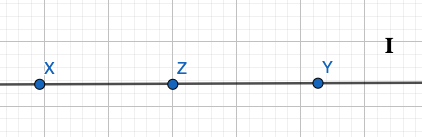
\includegraphics[width=5cm]{Intervallo.png}
	\caption{Tutto il segmento fra x e y deve stare in I}
	\label{fig:intervallo}
\end{wrapfigure}
I è un intervallo se ogni \emph{ogni} punto che prendo tra gli estremi dell'intervallo, questo appartiene all'intervallo stesso.
\\\\\\\\\\
\begin{example}
Esempi di intervalli.\\ \\
Questo caso \textbf{è un intervallo} \hspace{3.2cm} Questo caso \textbf{non è un intervallo} fra A e D.
\begin{figure}[h!]
    \vspace{-10pt}
    \begin{subfigure}{.5\textwidth}
        \hspace{-50pt}
        \centering
        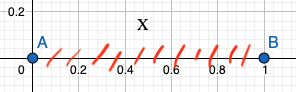
\includegraphics[width=6cm]{Esempio-intervallo-1.png}
        \caption{$A = \{x \in \mathbb{R} \: | \: 0<x<1\}$}
    \end{subfigure}
    \begin{subfigure}{.5\textwidth}
        \centering
        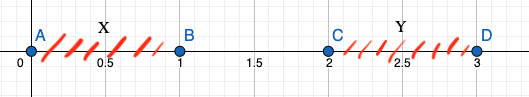
\includegraphics[width=7.5cm]{Esempio-intervallo-2.png}
        \caption{$C = \{x \in \mathbb{R} \: | \: 0<x<1 \: \vee \: z<x<3\}$}
    \end{subfigure}
\end{figure}
\end{example}

\newpage
\subsection{Notazione}
Con $a, b \in \mathbb{R}$ e con $a < b$ è possibile scrivere le notazioni in tabella \ref{tab:notazione-intervalli}.
\begin{table}[h!]
    \centering
    \setlength{\tabcolsep}{7pt}
    \renewcommand{\arraystretch}{2}
    \begin{tabular}{|c|c|c|} \hline
        [a, b] & Intervallo chiuso di estremi a e b & $\{x \in \mathbb{R} \: | \: a \leq x \leq b\}$ \\ \hline
        (a, b) & Intervallo aperto & $\{x \in \mathbb{R} \: | \: a < x < b\}$ \\ \hline
        [a, b) & Intervallo semi aperto a destra & $\{x \in \mathbb{R} \: | \: a \leq x < b\}$ \\ \hline
        (a, b] & Intervallo semi aperto a sinistra & $\{x \in \mathbb{R} \: | \: a < x \leq b\}$ \\ \hline
        [a, $+\infty$) & Semiretta chiusa a sinistra & $\{x \in \mathbb{R} \: | \: a \leq x\}$ \\ \hline
        ($-\infty$, b] & Semiretta chiusa a destra & $\{x \in \mathbb{R} \: | \: x \leq b\}$ \\ \hline
        ($-\infty$, $+\infty$) & Insieme di tutti i numeri $\mathbb{R}$ & $\{x \in \mathbb{R}\}$ \\ \hline
    \end{tabular}
    \caption{Notazione Intervalli}
    \label{tab:notazione-intervalli}
\end{table}
\newpage
\section{Array}
Una struttura dati molto conosciuta e chiamata array.
\begin{definition}[Array]
Gli array sono delle strutture dati omogenea, statiche e lineari implementate mediante un gruppo di celle contigue di memoria dello stesso tipo.
\end{definition}

Di seguito due esempi grafici di array uno di interi ed uno di stringhe, da notare sotto la posizione degli elementi nell'array che si conta partendo dallo 0.
\begin{figure}[h!]
    \centering
    \begin{subfigure}{.5\textwidth}
        \centering
        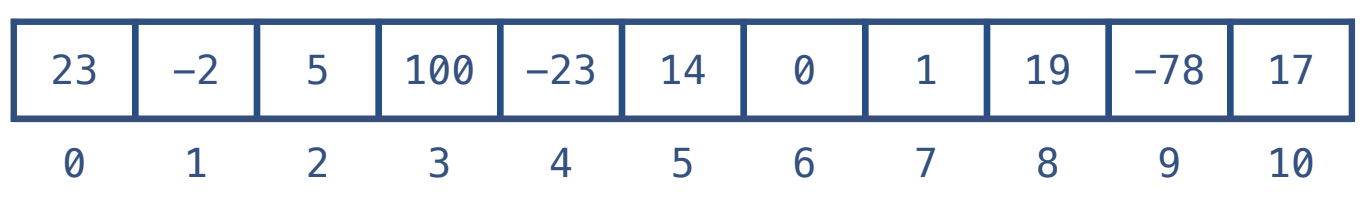
\includegraphics[width=9cm]{images/esempio-array-1.png}
        \caption{}
    \end{subfigure}
    \hfill
    \begin{subfigure}{.4\textwidth}
        \centering
        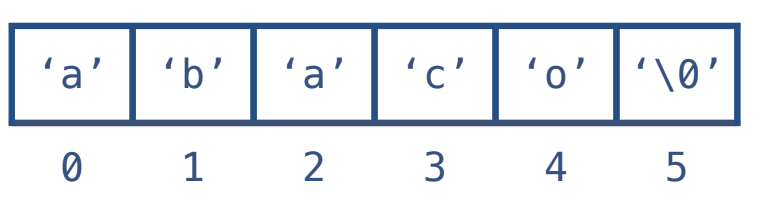
\includegraphics[width=6cm]{images/esempio-array-2.png}
        \caption{}
    \end{subfigure}
    \caption{In (a) un array lungo 11 di interi, in (b) un array lungo 6 di caratteri}
\end{figure}
\begin{note}
Nota che nell'array di caratteri sopra nell'ultima posizione c'è sempre $\setminus0$ (Null).
\end{note}
Negli array si accede mediante l'indice della posizione nella sequenza. Si possono inoltre effetturare sugli elementi tutte le operazioni definte sul tipo corrispondete agli elementi dell'array.
\begin{example}
Alcuni esempi di accesso ed operazioni su gli arrey sopra:
\begin{itemize}
    \item a[6] == 0 \hspace{.5cm} a[3] == 100 \hspace{.5cm} b[2] == 'a' 
    \item a[4] = a[5] + a[7] \: \: (a[5] == 14, a[7] == 1, quindi il risultato sarà 14 + 1 = 15)  
\end{itemize}
\end{example}

Inoltre possiamo dire che gli array sono allocati in memoria quando il controllo del flusso a tempo di esecuzione entra nel blocco in cui sono definiti e sono distrutti quando il controllo esce dal blocco.\\\\
Il nome dell'array è una variabile che contiene la locazione di memoria in cui è memorizzata la prima cella. Essendo che le celle sono contigue e hanno tutte lo stesso tipo basta infatti conoscere la posizione della prima cella per poi, tramite una semplice operazione algebrica di somma, accedere a quelle successive. In generale possiamo scrivere che:
\begin{center}
    $a[i] \: \: = \: \: \sigma(\rho(a) + size(type(a)) \times i)$
\end{center}
\begin{example}
Se abbiamo un array di lunghezza 11, ed chiamiamo la prima locazione (quella dove è contenuto il primo elemento dell'array) loc1, per raggiungere la posizione numero 10 basterà eseguire l'operazione loc1 + 32*10.
\end{example}
Questo consente l'accesso diretto agli elementi degli array con una sola operazione indipendentemente dalla lunghezza dell'array (consto di accesso costante). 

\subsection{BinarySearch}
\textbf{Problema:} Dato un elemento (o chiave) k, determinare se esiste all’interno di un array ordinato A di n elementi. Se l’elemento esiste, si restituisce la sua posizione, altrimenti -1. Soluzione con ricerca binaria.\\
\textbf{Proprietà:} $\forall i \in [0..n-1] \: . \: A[i] \leq A[i+1]$\\
Questa proprietà dice che l'array A deve essere obbligatoriamente ordinato, sennò la ricerca binaria non potrà esser fatta.
\begin{figure}[h!]
    \vspace{-10pt}
    \centering
    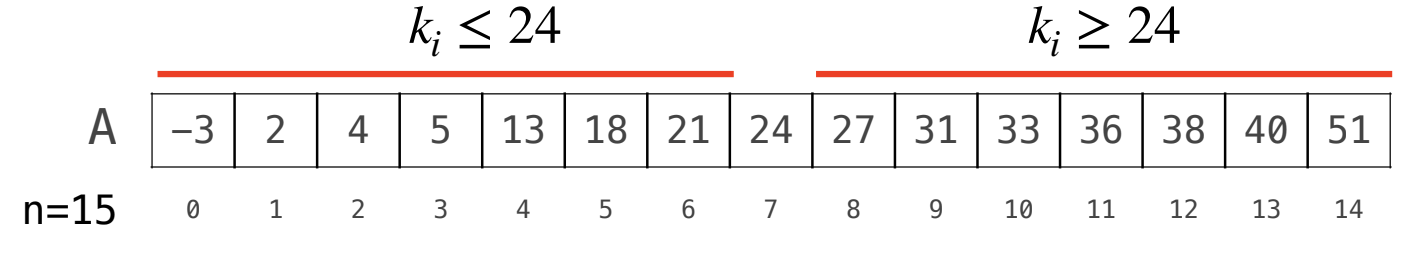
\includegraphics[width=9cm]{images/binary-search.png}
    \vspace{-8pt}
    \caption{Array A in BinarySearch}
    \label{fig:binary-search}
\end{figure}

\subsubsection{Codice dell'algoritmo}
\begin{lstlisting}[language=Javascript, caption=Codice BinarySearch]
function binSearch(k,A) {
    var pos:Int = -1;
    var sin:int = 0;
    var dx:Int = n - 1;
    while(sin <= dx && pos == -1){
        const cen:int = (sin + dx)/2;
        if (A[cen] == k) {pos = cen}
        else if (k < A[cen]) {dx = cen - 1}
        else {sin = cen + 1}
    }
    return pos;
}
\end{lstlisting}
Di seguito una spiegazione del funzionamento dell'algoritmo:
\begin{itemize}
    \item \textbf{Righe 2-4:} Andiamo ad inizializzare 3 variabili: "pos" che indicherà la posizione dell'elemento da cercare, viene inizializzata a -1 perché nel caso non si trovasse ritorna così -1. \\
    "Sin" che indica il capo sinistro della posizione che stiamo analizzando, e "dx" che indica il capo destro, sono entrambi inizialmente inizializzati come gli estremi dell'array.
    \item \textbf{Riga 5:} La condizione del while dice in sintesi che finché non abbiamo trovato il valore (pos == -1) e finchè "sin" e "dx" non si scambiano (che vorrebbe dire che abbiamo finito le iterazioni possibili), continuare a ciclare.
    \item \textbf{Righe 6-9:} All'interno del while quello che andiamo a fare e prendere il centro della porzione dell'array che stiamo considerando (inizialmente il centro dell'interno array) e vedere se il valore che dobbiamo cercare si trova in quella posizione, e in tal caso finiamo, è minore, e quindi si troverà alla sinistra del centro, o maggiore, in tal caso si troverà alla destra; nel caso non si sia trovato ci spostiamo ad analizzare la parte destra o sinistra asseconda del risultato. Eseguiamo questa operazioni finché è consentito dal ciclo.
\end{itemize}
\begin{note}
Nota che a noi non ci importa se la porzione è pari o dispari, quello che ci ritornerà esclude il resto.
\end{note}
\begin{example}
Esempio con l'array in figura \ref{fig:binary-search} cercando il valore 18.
\begin{table}[h!]
    \centering
    \setlength{\tabcolsep}{10pt}
    \renewcommand{\arraystretch}{1.8}
    \begin{tabular}{|c|c|c|c|c|}
    \hline
        pos & sin & dx & cen & A[cen]  \\\hline
        -1 & 0 & 14 & 7 & 24  \\\hline 
        -1 & 0 & 6 & 3 & 5  \\\hline
        -1 & 4 & 6 & 5 & \textbf{18}  \\
    \hline
    \end{tabular}
    \hspace{1cm}
    \begin{tabular}{|c|c|}
    \hline
        Iterazioni & Dimensione A \\\hline
        1 & n \: = \: n$/2^0$  \\\hline 
        2 & n/2 \: = \: n$/2^1$ \\\hline
        3 & n/4 \: = \: n$/2^2$ \\\hline
        ... & ... \\
    \hline
    \end{tabular}
    \caption{Esempio di funzionamento dell'algoritmo a sinistra e numero iterazione a destra}
\end{table}
\end{example}

\subsubsection{Calcolo caso pessimo e migliore}
Per calcolare il caso pessimo partiamo guardando la tabella sopra, notiamo che in questo algoritmo verranno eseguite $n/2^i$ operazioni, quindi il massimo possibile dipende da quanto è grande $i$. Per andare a trovare $i$ basta:
\begin{center}
    $n/2^i = 1$ \hspace{.3cm} $n = 2^i$ \hspace{.3cm} $\log_2n = \log_22^i$ \hspace{.3cm} $i = \log_2n \in O(\log_n)$
\end{center}
Questo caso è o quando k si trova agli estremi o quando k non c'è nell'array, e quindi ritorna -1.
\newpage
\section{Funzioni}
\begin{definition}[Funzione]
- $f: A \longrightarrow B$: \\
Dati due insiemi A, B, detti corrispettivamente dominio e codominio, una funzione è una "legge" o "regola" che associa ad ogni elemento di $a \in A$ uno ed uno solo elemento di B, che si denota con f(a).
\end{definition}
\begin{note}
Tipicamente in questo corso le funzioni saranno date come formule del tipo $f(x) = x^2 - 7x - e^x$ andando poi a specificare dominio e codominio in questo modo $f: \mathbb{R} \longrightarrow \mathbb{R}$
\end{note}
\begin{example}
    Esempi funzioni:
    \begin{itemize}
        \item $g(x) = x^2 - 7x - e^x$ \hspace{.3cm} $g(0,+\infty) \longrightarrow \mathbb{R}$
        \item $g(x) = x^2$ \hspace{.3cm} $g(0, +\infty) \longrightarrow (0, +\infty)$. \hspace{.3cm}Va bene perché $x^2 > 0$ per qualsiasi valore di x.
        \item $h(x) = x^2$ \hspace{.3cm} $h(0, +\infty) \longrightarrow (-\infty, 0)$. \hspace{.3cm}Questa forma non va bene non definendo una funzione perché la formula non mi da numeri di $(-\infty, 0)$.
        \item $h(x) = x^2$ \hspace{.3cm} $h(0, +\infty) \longrightarrow (-\infty,1)$ \hspace{.3cm}Non va bene perché se preindiamo x=3 $f(3) = 9$ e 9 non fa parte del codominio. 
    \end{itemize}
\end{example}
Una funzione $f: A \longrightarrow B$ con $A,B \in \mathbb{R}$ ha un \textbf{grafico} che si indica come:
\begin{equation}
    graph(f) = \{(a,b) \in A \:X\: B\ \:|\: b = f(a)\}
\end{equation}
\begin{wrapfigure}[8]{l}{7cm}
    \centering
    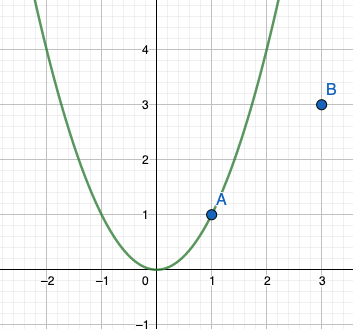
\includegraphics[width=4.5cm, height=4cm]{Esempio-grafico.png}
    \caption{$f(x) = x^2$ con $f: \mathbb{R} \longrightarrow \mathbb{R}$}
    \label{fig:esempio-grafico}
\end{wrapfigure}
\begin{example}
Esempio punto sulla funzione
\begin{itemize}
    \item Il punto A sta sul grafico si $f(x) = x^2$ esattamente quando $y = x^2$.
    \item Il punto B non sta sul grafico quindi $y \neq x^2$.
\end{itemize}
\end{example}
\begin{note}
    A X B $\subseteq \mathbb{R}$ X $\mathbb{R}$. Dove R X R = $R^2$.
\end{note}
\begin{example}
A e B = $(0, +\infty)$, da qui vediamo che A X B rappresenta il primo quadrante.\\\\
\end{example}

\subsection{Immagine}
\begin{definition}[Immagine]
Prendendo $f: A \longrightarrow B$ e $D \subseteq A$ l'immagine di D tramite f è il sottoinsieme $f(D) \subseteq B$ costituito dagli elementi f(d) dove $d \in D$.
\end{definition}
\begin{example}
    Esempi immagine:
    \begin{itemize}
        \item Immagine di A, $f(A) \subseteq B$ si chiama anche immagine della funzione.
        \item $f(x) = x^2$, $f: \mathbb{R} \longrightarrow \mathbb{R}$ \hspace{.2cm} immagine di g è $[0, +\infty)$ perché $x^2 \geq 0 \: \forall \: x \in \mathbb{R}$.
        \item $g(x) = x?2$, $g:[2, +\infty) \longrightarrow \mathbb{R}$ \hspace{.2cm} l'immagine di g è $[4, +\infty]$ perché se si calcola il punto minore del dominio, cioè 2, torna $g(2) = x^2$ che è uguale a 4, da lì possiamo prendere tutti i punti.
    \end{itemize}
\end{example}

\subsection{Suriettiva}
\begin{definition}[Suriettiva]
Una funzione si dice suriettiva quando ogni elemento del codominio è immagine di almeno un elemento del dominio. Quindi prendendo una f(x), per che sia suriettiva deve l'immagine I essere uguale ad un valore, $I(f) = b$.
\end{definition}
\begin{example}
    Esempi funzioni suriettive:
    \begin{itemize}
        \item $f(x) = x^2$, $f: \mathbb{R} \longrightarrow \mathbb{R}$ non è suriettiva perché tutti i valori del codominio $y < 0$ non hanno un rispettivo nel dominio.
        \item $g(x) = x^2$, $g: \mathbb{R} \longrightarrow (0, +\infty)$ lo è perchè andiamo a restringere il codominio ai punti che hanno un corrispettivo nel dominio.
    \end{itemize}
\end{example}

\subsection{Iniettiva}
\begin{definition}[Iniettiva]
Una funzione iniettiva è una funzione che associa, a elementi distinti del dominio, elementi distinti del codominio. Quindi prendendo una f(x) è iniettiva se prendendo due valori $x_1, x_2$ dove $x_1 \neq x_2 \Longrightarrow f(x_1) \neq f(x_2)$. (Input diversi danno output diversi).
\end{definition}
\begin{example}
    Esempi funzioni iniettiva:
    \begin{itemize}
        \item $f(x) = x^2$, $f: \mathbb{R} \longrightarrow \mathbb{R}$ non è iniettiva perché se prendiamo $x_1 = 1$ e $x_2 = -1$ $f(x1) = f(x2).$
        \item $g(x) = x^2$, $g: [0, +\infty) \longrightarrow \mathbb{R}$ è invece iniettiva perché non consideriamo i valori negativi.
    \end{itemize}
\end{example}

\subsection{Biunivoca}
\begin{definition}[Biunivoca]
Una funzione si definisce biunivoca o bigettiva se è sia iniettiva che suriettiva.
\end{definition}

\subsection{Invertibile}
\begin{definition}[Invertibile]
Se una funzione è biunivoca si dice che tale funzione è anche invertibile.
\end{definition}
\begin{wrapfigure}{l}{6cm}
    \centering
    \includegraphics[width=5cm, height=4cm]{Esempio-invertibilità.png}
    \caption{$f(x) = x^2$ e $g(x) = \sqrt{x}$}
    \label{fig:esempio-invertibilità}
\end{wrapfigure}
Se f è una funzione invertibile i grafici di f e di $f^i$ (la funzione inversa) sono simmetrici rispetto alla retta y=x cioè alla bisettrice del primo e del terzo quadrante. \\
\begin{example}
Se vediamo nell'immagine [\ref{fig:esempio-invertibilità}] prendendo l'inverso della funzione $f(x) = x^2$ definita in $[0, +\infty] \longrightarrow \mathbb{R}$ e cioè la funzione $g(x) = \sqrt{x}$ è simmetrica.
\\ \\ \\ \\ \\
\end{example}

\subsection{Funzioni Monotone}
\begin{definition}[Monotone]
Dato un insieme $A \in \mathbb{R}$ e $x_1, x_2 \in A$ con $x_1 < x_2$ se $\forall x_1, x_2$ risulta ciò che è scritto in Tabella \ref{tab:monotone}.
\end{definition}
\begin{table}[h!]
    \centering
    \setlength{\tabcolsep}{6pt}
    \renewcommand{\arraystretch}{1.7}
    \begin{tabular}{|c|c|}
        \hline
        \textbf{[1] Strettamente Crescente} & $f(x_1) < f(x_2) $ \\ \hline
        \textbf{[2]Debolmente Crescente} & $f(x_1) \leq f(x_2) $ \\ \hline
        \textbf{[3]Strettamente Decrescente} & $f(x_1) > f(x_2) $ \\ \hline
        \textbf{[4]Debolmente Decrescente} & $f(x_1) \geq f(x_2) $ \\ \hline
    \end{tabular}
    \caption{Definizioni funzioni crescenti e decrescenti}
    \label{tab:monotone}
\end{table}
Andando a considerare la Tabella \ref{tab:monotone} possiamo dire che:
\begin{itemize}
    \item \textbf{Strettamente monotona} nei casi [1] e [3] della tabella.
    \item \textbf{Debolmente monotona} nei casi [2] e [4] della tabella.
\end{itemize}

\begin{example}
    Esempi funzioni crescenti e decrescenti:\\
    \begin{figure}[h!]
        \begin{subfigure}{.5\textwidth}
            \centering
            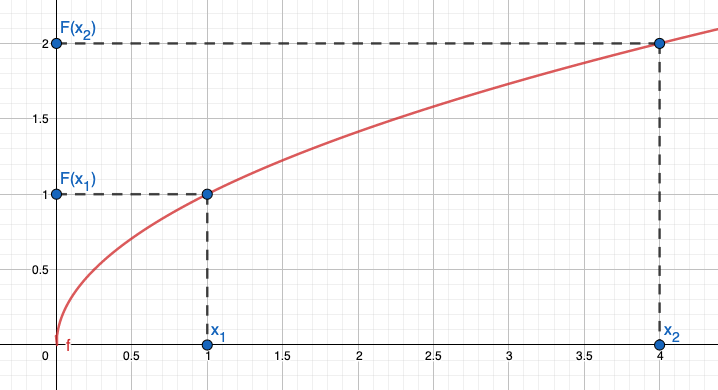
\includegraphics[width=6cm, height=4cm]{funzione-crescente.png}
            \caption{$f(x_1) < f(x-2)$ quindi è crescente}
            \label{fig:funzione-crescente}
        \end{subfigure}
        \begin{subfigure}{.5\textwidth}
            \centering
            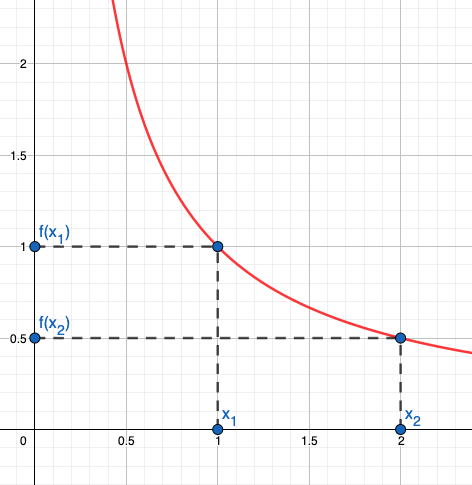
\includegraphics[width=6cm, height=4cm]{funzione-decrescente.png}
            \caption{$f(x_1) > f(x-2)$ quindi è decrescente}
            \label{fig:funzione-decrescente}
        \end{subfigure}
    \end{figure}
    \\Possiamo anche federe dalle immagini [\ref{fig:funzione-crescente}] [\ref{fig:funzione-decrescente}] che:
    \begin{itemize}
        \item Se f(x) è \textbf{crescente} l'ordinamene verrà \textbf{mantenuto}.
        \item Se f(x) è \textbf{decrescente} l'ordinamento verrà \textbf{invertito}.\\
    \end{itemize}
\end{example}

\begin{observation}
    Osservazione sul rapporto incrementale:\\
\end{observation}
\begin{wrapfigure}[8]{l}{8cm}
    \vspace{-15pt}
    \centering
    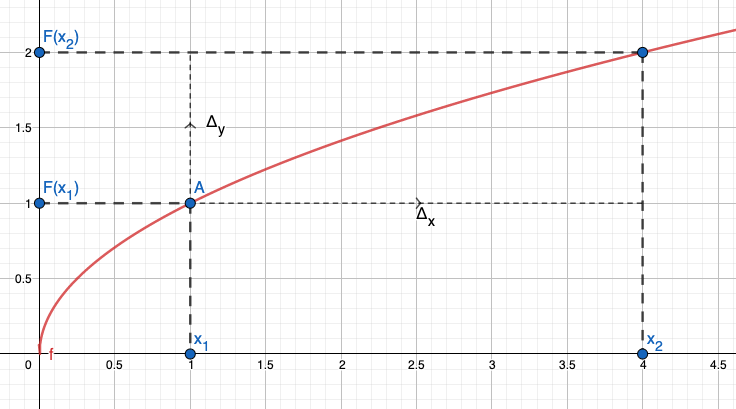
\includegraphics[width=6.7cm]{rapporto_incrementale.png}
    \caption{$\frac{\Delta_y}{\Delta_x}$}
    \label{fig:esempio-invertibilità}
\end{wrapfigure}
f(x) è strettamente crescente se e solo se il \textbf{rapporto incrementale}\footnote{I rapporto incrementale misura quanto il punto della f si sposta in verticale in rapporto a quanto abbiamo l'asciasse in orizzontale.} è maggiore di 0:
\begin{equation}
    \frac{f(x_1) - f(x_2)}{x_1 - x_2} > 0
\end{equation}
\begin{note}
    Il denominatore ed il numeratori devono essere concordi per fare in modo che il rapporto incrementale sia maggiore di 0 e quindi la funzione crescente. \\ \\\\
\end{note}
Continuando ad analizzare il rapporto incrementale possiamo ricavare anche i casi in cui una funzione e strettamente decrescente o debolmente crescente o debolmente decrescente. Puoi vedere tutte le casistiche nella tabella \ref{tab:analisi-rapporto-incrementale}.
\begin{table}[h!]
    \centering
    \setlength{\tabcolsep}{7pt}
    \renewcommand{\arraystretch}{2}
    \begin{tabular}{|c|c|}
        \hline
        Strettamente Crescente & $\frac{f(x_1) - f(x_2)}{x_1 - x_2} > 0$\\ \hline
        Strettamente Decrescente & $\frac{f(x_1) - f(x_2)}{x_1 - x_2} < 0$ \\ \hline
        Debolmente Crescente & $\frac{f(x_1) - f(x_2)}{x_1 - x_2} \geq 0$ \\ \hline
        Debolmente Decrescente & $\frac{f(x_1) - f(x_2)}{x_1 - x_2} \leq 0$ \\ \hline
    \end{tabular}
    \caption{Analisi rapporto incrementale}
    \label{tab:analisi-rapporto-incrementale}
\end{table}
\begin{observation}
    Se una funzione f(x) è strettamente crescente è a sua volta anche debolmente crescente, mentre una funzione f(x) se è debolmente crescente non è strettamente crescente perché aggiunge una casistica che sarebbe $f(x_1) = f(x_2)$. 
\end{observation}
\begin{example}
    Casistica particolare:\\
    Data $f(x)=\frac{1}{x}$, \hspace{.3cm} $f: \mathbb{R} \: \setminus \: \{0\} \longrightarrow \mathbb{R} \: \setminus \: \{0\}$. Funzione rappresentata nell'immagine [\ref{fig:esempio-particolare}].
    \begin{figure}[h!]
        \centering
        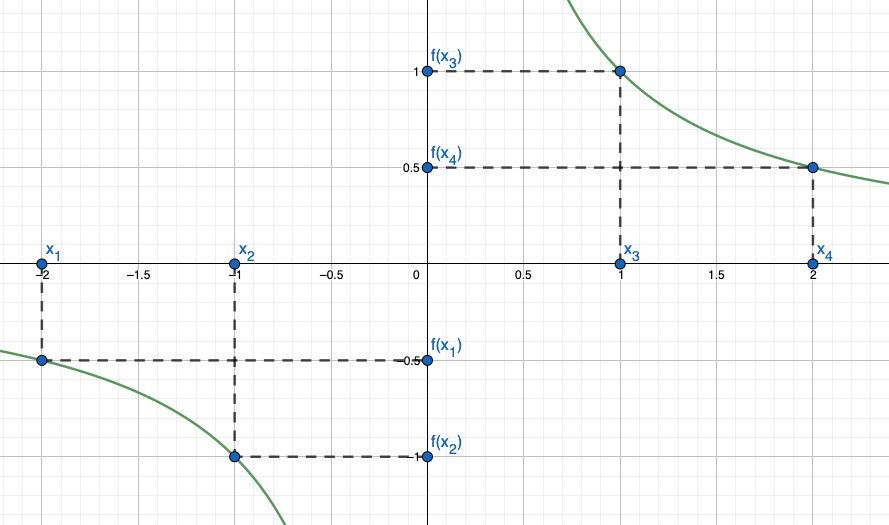
\includegraphics[width=8.7cm]{esempio-particolare.png}
        \caption{$f(x)=\frac{1}{x}$, \hspace{.3cm} $f: \mathbb{R} \: \setminus \: \{0\} \longrightarrow \mathbb{R} \: \setminus \: \{0\}$}
        \label{fig:esempio-particolare}
    \end{figure}
    \\Possiamo vedere che:
    \begin{itemize}
        \item f(x) è strettamente decrescente in $(0, +\infty)$.\\
        Quindi se andiamo a prendere $0 < x_3 < x_4$ abbiamo che $f(x_3) > f(x_4)$.
        \item f(x) è strettamente decrescente in $(-\infty, 0)$.\\
        Quindi se andiamo a prendere $x_1 < x_2 < 0$ abbiamo che $f(x_1) > f(x_2)$.
    \end{itemize}
    Se però andiamo a considerare tutto $\mathbb{R} \: \setminus \: \{0\}$, e quindi prendiamo i punti $x_1 < 0 < x_4$ vediamo che $f(x_1) < f(x_4)$.
    In conclusione si può dire quindi che $f(x)=\frac{1}{x}$) è decrescente in $(-\infty, 0)$ e in $(0, +\infty)$ ma non lo è in tutto $\mathbb{R} \: \setminus \: \{0\}$.
\end{example}

\subsubsection{Composizione con funzioni monotone}
\begin{note}
     Il simbolo della composizione è "$\circ$", come $f \circ g$.
\end{note}
Prendendo i considerazioni 3 insiemi A, B, C tali che $A, B, C \subset \mathbb{R}$ e 2 funzioni f(x) e g(x) così definitine: \hspace{.2cm} $f: A \longrightarrow B$, $g: B \longrightarrow C $.
\begin{enumerate}
    \item Se f è crescente e g è crescente allora $g \circ f$ è crescente.
    \item Se f è crescente e g è decrescente allora $g \circ f$ è decrescente. (Vale anche l'inverso).
    \item Se f è decrescente e g è decrescente allo $g \circ f$ è crescente. 
\end{enumerate}
\begin{example}
    $h(x) = e^{x^3}$\\
    La funzione h si ottiene dalla composizione di:
    \begin{itemize}
        \item $f: \mathbb{R} \longrightarrow \mathbb{R}$ \hspace{.3cm} $f(x) = x^3$. Funzione crescente.
        \item $g: \mathbb{R} \longrightarrow \mathbb{R}$ \hspace{.3cm} $g(t) = e^t$. Funzione decrescente.
    \end{itemize}
    Quindi possiamo scrivere $h(x) = e^{x^3}$ come: \hspace{.3cm} $e^{f(x)} \: \: = \: \: g(f(x)) \: \: = \: \: (g \circ f)(x)$
    Inoltre visto che f è crescente e g è crescente, h è strettamente crescente 
\end{example}
\begin{observation}
    Se prendiamo una funzione f(x) strettamente monotona, allora f(x) è iniettiva. Questa condizione è vera ma NON lo è viceversa: una funzione f(x) iniettiva NON è per forza strettamente monotona. 
\end{observation}
\begin{example}
    Se prendiamo una f(x) tale che: \hspace{.3cm} $f(x) = \frac{1}{x}$ \hspace{.3cm} $\mathbb{R} \setminus \{0\} \longrightarrow \mathbb{R} \setminus \{0\}$
    \\Possiamo vedere rifacendoci all'esempio in figura [\ref{fig:esempio-particolare}] che f è iniettiva ma non monotona.
\end{example}

\subsection{Insieme di definizione}
\begin{definition}[Insieme di definizione]
    Prendendo una funzione f(x) l'insieme di definizione o dominio naturale di una funzione è il più grande sottoinsieme di $\mathbb{R}$ dove ha senso la funzione f(x).
\end{definition}
\begin{example}
    $f(x) = \frac{1}{x}$ \hspace{.3cm} L'insieme di definizione è $\mathbb{R} \setminus \{0\}$
\end{example}

\subsection{Funzioni pari e dispari}
\begin{definition}[Pari]
    La funzione è \textbf{Pari} se $f(x) = f(-x) \: \forall x$ nel dominio di $f \longrightarrow f$.
\end{definition}
\begin{definition}[Dispari]
    La funzione è \textbf{Dispari} se $f(x) = -f(-x) \: \forall x$ nel dominio di $f \longrightarrow f$.
\end{definition}
\begin{note}
    Il dominio di f deve essere tale che se $x \in Dominio$ allora $-x \in Codominio$.\\
\end{note}
\begin{example}
Esempio funzioni pari e dispari.\\
\end{example}
$f(-x) = (-x)^2 = x^2 = f(x)$, f(x) è \textbf{pari}: \hfill $f(-x) = (-x)^2 = x^2 = -f(x)$, f(x) è \textbf{dispari}:
\begin{figure}[h!]
    \vspace{-1pt}
    \begin{subfigure}{.5\textwidth}
        \centering
        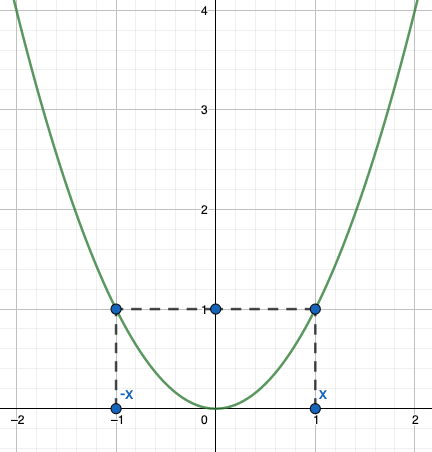
\includegraphics[width=3cm]{funzione-pari.png}
        \caption{$f(x) = x^2$, \hspace{.2cm} graph(f) con f pari}
    \end{subfigure}
    \begin{subfigure}{.5\textwidth}
        \centering
        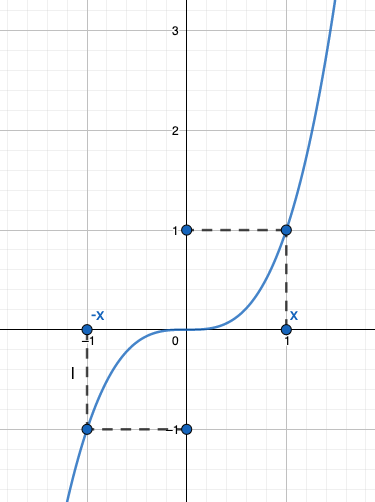
\includegraphics[width=2.5cm]{funzione-dispari.png}
        \caption{$f(x) = x^3$, \hspace{.2cm} graph(f) con f dispari}
    \end{subfigure}
\end{figure}

\subsection{Funzione periodica}
\begin{definition}[Periodicità]
    Una funzione f(x) si dice periodica di periodo $P \in \mathbb{R}$ se $\forall x \: \: f(x + P) = f(x)$. 
\end{definition}
\begin{wrapfigure}{r}{9cm}
    \vspace{-15pt}
    \centering
    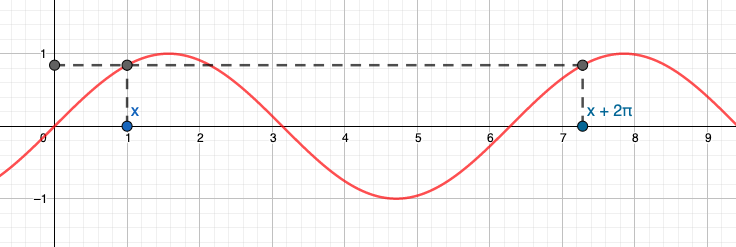
\includegraphics[width=7cm]{funzione-periodica.png}
    \caption{$sin(x) = sin(x + 2\pi)$}
    \label{fig:funzione-periodica}
\end{wrapfigure}
Inoltre il dominio di f(x) deve essere tale che $x \in$ Dominio è uguale e a $x + P \in$ codominio.
\begin{example}
In figura [\ref{fig:funzione-periodica}] un esempio di funzione periodica.\\\\
\end{example}

\newpage
\subsection{Funzioni Elementari}
\subsubsection{Retta}
\textbf{Funzione retta:} $f(x) = ax + b$. \hspace{.3cm} $a,b \in \mathbb{R}$ \\ Dove la "a" si dice coefficiente angolare, ed indica la pendenza della retta mentre la lettera "b" si chiama termine noto, ed indica il punto di incontro con l'asse Y.

\subsubsection{Esponente positivo o negativo}
\textbf{Fun. Esp. positivo:} $f(x) = x^k$, $k \in \mathbb{N}$. \hfill \textbf{Fun. Esp. negativo:} $f(x) = x^k$, $k \in \mathbb{N}$, $k < 0$.
\begin{figure}[h!]
    \begin{subfigure}{.5\textwidth}
        \centering
        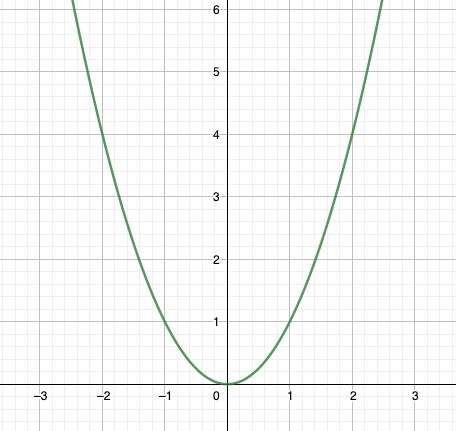
\includegraphics[width=4cm, height=3.5cm]{parabole.png}
        \caption{con k pari}
        \label{fig:esponente-positivo-pari}
    \end{subfigure}
    \begin{subfigure}{.5\textwidth}
        \centering
        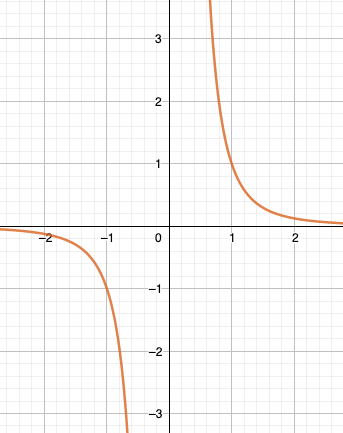
\includegraphics[width=4cm, height=3.5cm]{esponente-negativo-dispari.png}
        \caption{con k dispari}
        \label{fig:esponente-positivo-dispari}
    \end{subfigure}
\end{figure}
\begin{figure}[h!]
    \vspace{-5pt}
    \begin{subfigure}{.5\textwidth}
        \centering
        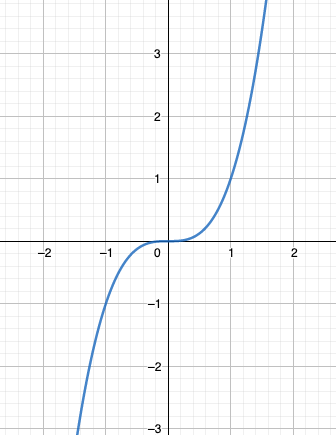
\includegraphics[width=4cm, height=3.7cm]{esponente-dispari.png}
        \caption{con k pari}
        \label{fig:esponente-negativo-pari}
    \end{subfigure}
    \begin{subfigure}{.5\textwidth}
        \centering
        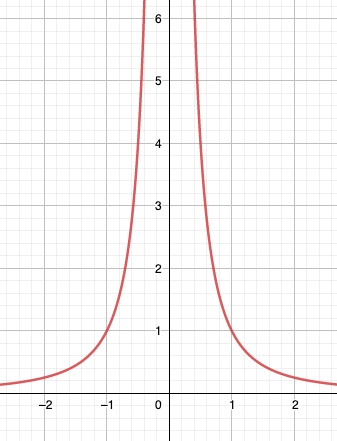
\includegraphics[width=4cm, height=3.5cm]{esponsente-negativo-pari.png}
        \caption{con k dispari}
        \label{fig:esponente-negativo-dispari}
    \end{subfigure}
\end{figure}
\begin{observation}
    \textbf{k pari:} Le funzioni con il k pari sono funzioni pari e hanno tutte una forma simile a quella in figura [\ref{fig:esponente-positivo-pari}] per le funzioni con k positive e per le funzioni con k negativo figura [\ref{fig:esponente-negativo-pari}].
\end{observation}
\begin{observation}
    \textbf{k dispari:} Le funzioni con il k positivo e dispari sono funzioni dispari e hanno tutte una forma simile a quella in figura [\ref{fig:esponente-positivo-dispari}] per le funzioni con k positive e per le funzioni con k negativo figura [\ref{fig:esponente-negativo-dispari}].
\end{observation}

\subsubsection{Radici o esponente fratto}
\textbf{Funzionane radici o esponente fratto:} $f(x) = x^{\frac{p}{q}}$ o $f(x) = \sqrt[q]{x^p}$  \: \: con  \: \:  $p, q \in \mathbb{N}$ \: \: e  \: \:  $q \neq 0$. \footnote{In matematica è possibile scrivere una un esponente fratto come radice mettendo il numeratore al radicando della radice e il denominatore all'indice: $x^{\frac{p}{q}} \: = \: \sqrt[q]{x^p}$}
\begin{figure}[h!]
    \begin{subfigure}{.5\textwidth}
        \centering
        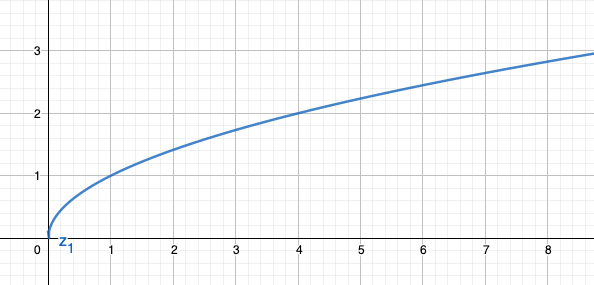
\includegraphics[width=6.3cm]{radice-pari.png}
        \caption{con q pari}
        \label{fig:radice-pari}
    \end{subfigure}
    \begin{subfigure}{.5\textwidth}
        \centering
        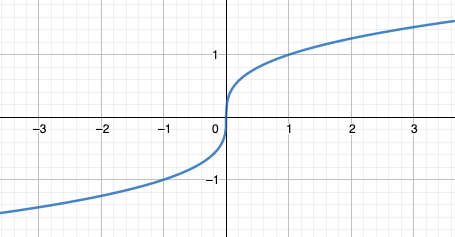
\includegraphics[width=6cm]{radice-dispari.png}
        \caption{con q dispari}
        \label{fig:radice-dispari}
    \end{subfigure}
\end{figure}
\begin{note}
    p e q non possono essere entrambi pari perché in tal caso sono divisibili fra di loro e quindi portabili ad una forma ridotta.
\end{note}
\begin{observation}
    \textbf{q pari:} Le funzioni con il q pari ha dominio $ x \geq 0$ ed è invertibile sono come funzione $f: [0, +\infty) \longrightarrow [0, +\infty)$. È rappresentata in figura [\ref{fig:radice-pari}].
\end{observation}
\begin{observation}
    \textbf{q dispari:} Le funzioni con il q positivo ha dominio $x \in \mathbb{R}$ ed è ugualmente invertibile su tutto $\mathbb{R}$, è inoltre una funzione dispari. È rappresentata in figura [\ref{fig:radice-dispari}].\\
\end{observation}

\subsubsection{Esponenziale}
\textbf{Funzione esponenziale:} $f(x) = a^x$ con $a \in \mathbb{R}$, \: \: $a > 0$, \: \: $a \neq 1$ \: \: $f: \mathbb{R} \longrightarrow (0, +\infty)$
\begin{figure}[h!]
    \begin{subfigure}{.5\textwidth}
        \centering
        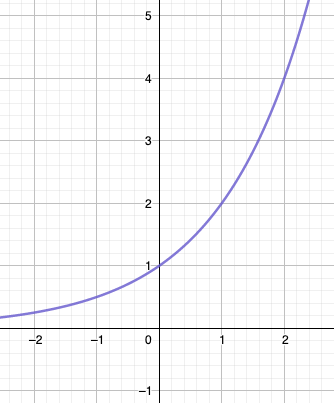
\includegraphics[width=4cm]{esponenziale.png}
        \caption{con $a > 1$}
        \label{fig:esponenziale}
    \end{subfigure}
    \begin{subfigure}{.5\textwidth}
        \centering
        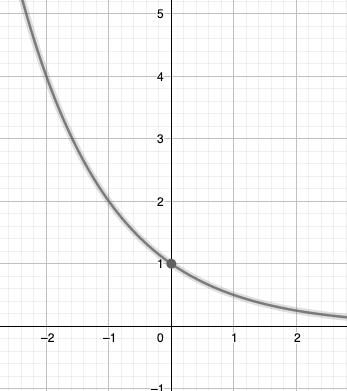
\includegraphics[width=4cm]{esponsenziale-base-minore.png}
        \caption{con $0 < a < 1$}
        \label{fig:esponsenziale-base-minore}
    \end{subfigure}
\end{figure}
\begin{note}
    La funzione esponenziale è sempre positiva.
\end{note}
\begin{observation}
    \textbf{$a > 1$:} La funzione è strettamente crescente, come in nell'immagine [\ref{fig:esponenziale}].
\end{observation}
\begin{observation}
    \textbf{$0 < a < 1$:} La funzione è decrescente, come in nell'immagine [\ref{fig:esponsenziale-base-minore}].
\end{observation}

\subsubsection{Logaritmo}
\textbf{Funzione logaritmo:} $f(x) = \log_a x$, \: \: $f: (0, +\infty) \longrightarrow \mathbb{R}$ \: \: (inversa dell'esponenziale).
\begin{figure}[h!]
    \begin{subfigure}{.5\textwidth}
        \centering
        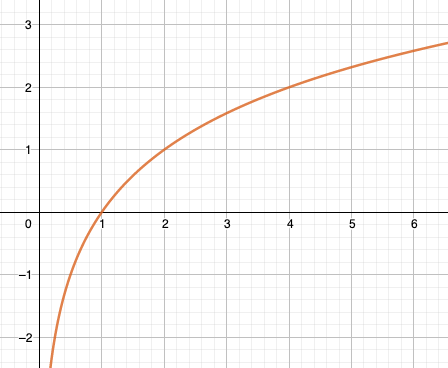
\includegraphics[width=5cm,height=4cm]{logaritmo.png}
        \caption{con $a > 1$}
        \label{fig:logaritmo}
    \end{subfigure}
    \begin{subfigure}{.5\textwidth}
        \centering
        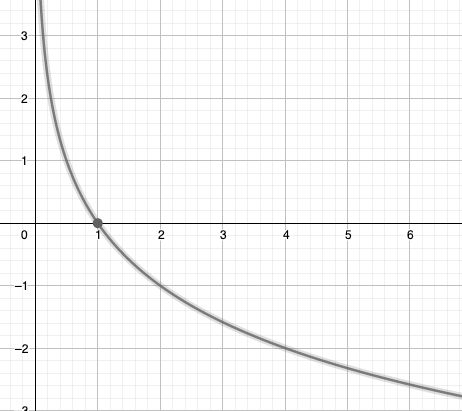
\includegraphics[width=5cm,height=4cm]{logaritmo-base-minore.png}
        \caption{con $0 < a < 1$}
        \label{fig:logaritmo-base-minore}
    \end{subfigure}
\end{figure}
\begin{observation}
    Casistica particolare - $f(x) = e^x$.\\
    In questa casistica se andiamo a ridurre il codominio la funzione esponenziale è invertibile. $f: \mathbb{R} \longrightarrow (0, +\infty)$.
    Il suo inverso è un caso particolare di logaritmo e di chiama \textbf{logaritmo naturale}. E si può scrive in due modi:
    \begin{itemize}
        \item $\ln{x}$: sarebbe logaritmo in base naturale.
        \item $\log x$: scrivendo il logaritmo senza la base intendiamo il logaritmo in base $e$.
    \end{itemize}
\end{observation}

\subsubsection{Seno e Arcoseno}
\textbf{Seno:} $f(x) = \sin x$, $f: \mathbb{R} \longrightarrow \mathbb{R}$. \hfill
\textbf{Arcoseno:} $f(x) = \arcsin x$, $f: [-1, 1] \longrightarrow [-\frac{\pi}{2}, \frac{\pi}{2}]$
\begin{figure}[h!]
    \begin{subfigure}{.5\textwidth}
        \centering
        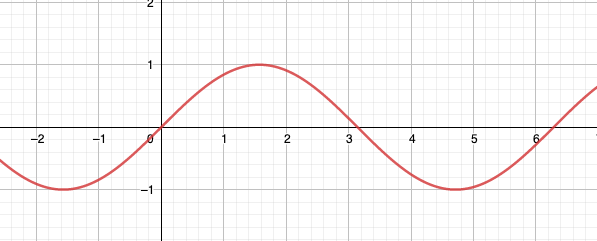
\includegraphics[width=6cm]{seno.png}
        \caption{$\sin{x}$}
        \label{fig:seno}
    \end{subfigure}
    \begin{subfigure}{.5\textwidth}
        \centering
        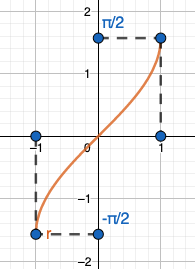
\includegraphics[width=2cm, height=2.3cm]{arcoseno.png}
        \caption{$\arcsin{x}$ o $\sin{x}^{-1}$}
        \label{fig:arcoseno}
    \end{subfigure}
\end{figure}

\begin{observation}
    \textbf{Sin(x):} La funzione $\sin{x}$ (immagine [\ref{fig:seno}]) è periodica per $2\pi$ quindi possiamo scrivere $\sin{(x+2\pi)} = \sin x \: \forall x \in \mathbb{R}$. Inoltre è suriettiva per codominio [-1, 1]. Se invece definiamo $f: [-\frac{\pi}{2}, \frac{\pi}{2}] \longrightarrow [-1, 1]$ la funzione $\sin x$ è strettamente crescente e suriettiva, quindi anche invertibile, e la sua inversa è appunto $\arcsin{x}$.
\end{observation}
\begin{observation}
    \textbf{Arcsin(x):} La funzione $\arcsin{x}$ è l'inverso del seno e può essere scritta anche come $f(x) = \sin{x}^{-1}$, è rappresentata nell'immagine [\ref{fig:arcoseno}].
\end{observation}

\subsubsection{Coseno e Arcocoseno}
\textbf{Coseno:} $f(x) = \cos{x}$, $f: \mathbb{R} \longrightarrow \mathbb{R}$. \hfill
\textbf{Arcocoseno:} $f(x) =\arccos{x}$, $f: [-1, 1] \longrightarrow [0, \pi]$
\begin{figure}[h!]
    \begin{subfigure}{.5\textwidth}
        \centering
        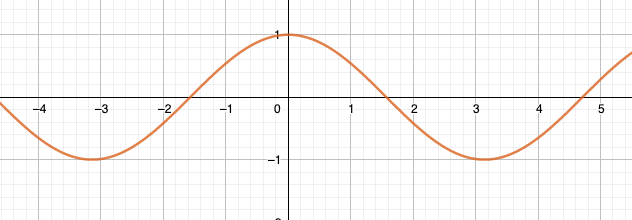
\includegraphics[width=6cm]{coseno.png}
        \caption{$\cos{x}$}
        \label{fig:coseno}
    \end{subfigure}
    \begin{subfigure}{.5\textwidth}
        \centering
        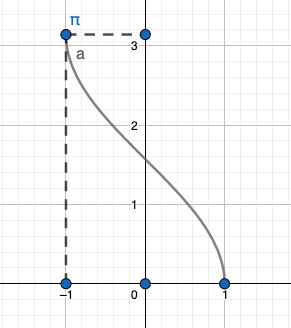
\includegraphics[width=3.5cm, height=2.7cm]{arcocoseno.png}
        \caption{$\arccos{x}$ o $\cos{x}^{-1}$}
        \label{fig:arcocoseno}
    \end{subfigure}
\end{figure}
\vspace{-5pt}
\begin{observation}
    \textbf{Cos(x):} La funzione $\cos{x}$, rappresentata nell'immagine [\ref{fig:coseno}], è periodica per $2\pi$ quindi possiamo scrivere $\cos{(x+2\pi)} = \cos x \: \forall x \in \mathbb{R}$. Inoltre è suriettiva per codominio [-1, 1]. Se invece definiamo $f: [0, \pi] \longrightarrow [-1, 1]$ la funzione $\cos x$ è suriettiva, quindi anche invertibile, e la sua inversa è appunto $\arccos{x}$.
\end{observation}
\begin{observation}
    \textbf{Arccos(x):} La funzione $\arccos{x}$ è l'inverso del seno e può essere scritta anche come $f(x) = \cos{x}^{-1}$ ed è rappresentata nell'immagine [\ref{fig:arcocoseno}].
\end{observation}

\subsubsection{Tangente e Arcotangente}
\textbf{Tangente:} $f(x) = \tan{x}$, $f: \mathbb{R} \longrightarrow \mathbb{R}$ \hfill
\textbf{Arcotangente:} $f(x) = \arctan{x}$, $f: \mathbb{R} \longrightarrow [-\frac{\pi}{2}, \frac{\pi}{2}]$
\begin{figure}[h!]
    \begin{subfigure}{.5\textwidth}
        \vspace{-20pt}
        \centering
        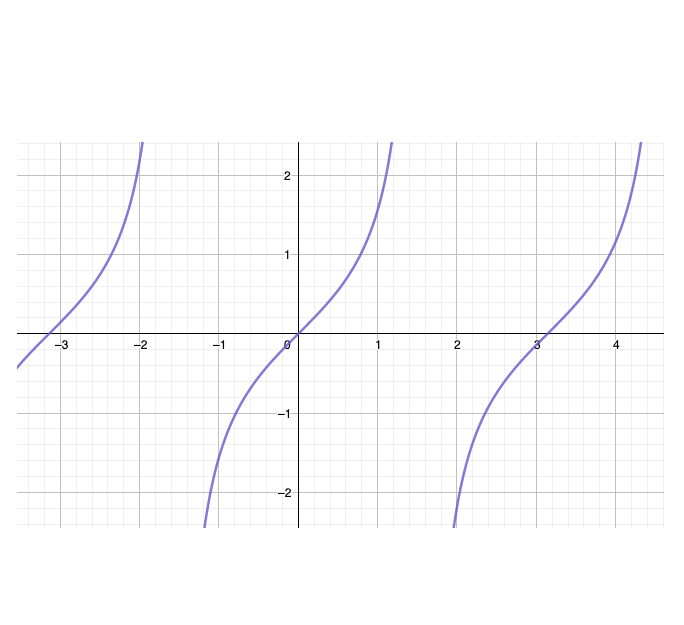
\includegraphics[width=4.2cm]{tangente.png}
        \vspace{-20pt}
        \caption{$\tan{x}$}
        \label{fig:tangente}
    \end{subfigure}
    \begin{subfigure}{.5\textwidth}
        \centering
        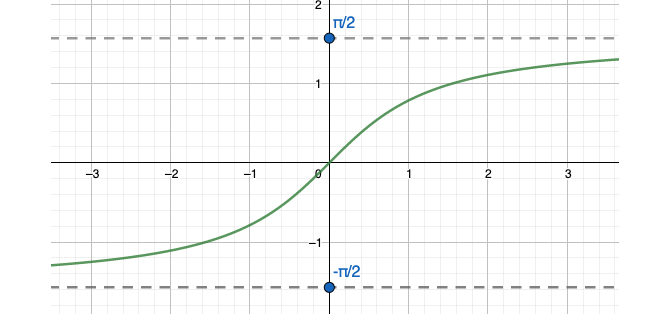
\includegraphics[width=5cm]{arcotangente.png}
        \caption{$\arctan{x}$ o $\tan{x}^{-1}$}
        \label{fig:arcotangente}
    \end{subfigure}
\end{figure}
\begin{observation}
    \textbf{Tan(x):} La funzione $\tan{x}$, rappresentata nell'immagine [\ref{fig:tangente}], può essere scritta anche come $\frac{\sin{x}}{\cos{x}}$, ha come dominio $\{x \in \mathbb{R} \: | \:  x \neq \frac{\pi}{2} + k\pi, \: k \in \mathbb{Z}\}$. La funzione tangente è fatta da infiniti intervalli, è quindi periodica per $\pi$; è di base non invertibile, ma se la ristringiamo in $f: [-\frac{\pi}{2}, \frac{\pi}{2}] \longrightarrow \mathbb{R}$ diventa biunivoca ed accetta la funzione inversa che è $\arctan{x}$.
\end{observation}
\begin{observation}
    \textbf{Arctan(x):} La funzione $\arctan{x}$, rappresentate nell'immagine [\ref{fig:arcotangente}], è inversa della funzione $\tan{x}$, può quindi essere scritta anche con la forma $\tan{x}^{-1}$.
\end{observation}
\newpage
\section{Gestione della memoria}
\subsection{Record di attivazione}
\begin{definition}
	è l'insieme di strutture dati e funzioni necessarie all'esecuzione dei programmi viene aggiunto al codice eseguibile dal compilatore.
\end{definition}
\begin{definition}[Activation record o stack frame]
	Contiene tutte le informazioni necessarie all'esecuzione del blocco o della funzione.
\end{definition}
\begin{definition}[Dynamic chain o call chain]
	Rappresenta la sequenza di chiamate e e serve a garantire il corretto ordine di esecuzione.
\end{definition}
\begin{definition}[Static chain]
	Implementa lo scoping statico e garantisce che i nomi siano referenziati rispettando la visibilità di variabili e funzioni.
\end{definition}
\begin{tabular} { |c|p{250px}|}
	\hline
	Puntatore catena dinamica  & Indirizzo del record di attivazione della funzione chiamante\\
	\hline
	Puntatore catena statica & Indirizzo del prossimo record di attivazione dove risolvere i nomi
		non presenti nel blocco corrente (implementazione dello scoping
		statico) \\
	\hline
	Indirizzo di ritorno & Indirizzo dell’istruzione da eseguire al termine della funzione/blocco corrente \\
	\hline
	Indirizzo risultato & Indirizzo nel record di attivazione del chiamante per memorizzare il risultato \\
	\hline
	Parametri & Spazio riservato alla associazione parametri formali - parametri attuali \\
	\hline
	Variabili locali & Spazio riservato alla allocazione delle variabili locali al blocco \\
	\hline
	Risultati temporanei & Spazio riservato alla allocazione delle variabili temporanee generate dal compilatore \\
	\hline
\end{tabular}
\subsection{Divisione della memoria}
\begin{figure}[h!]
	\centering
	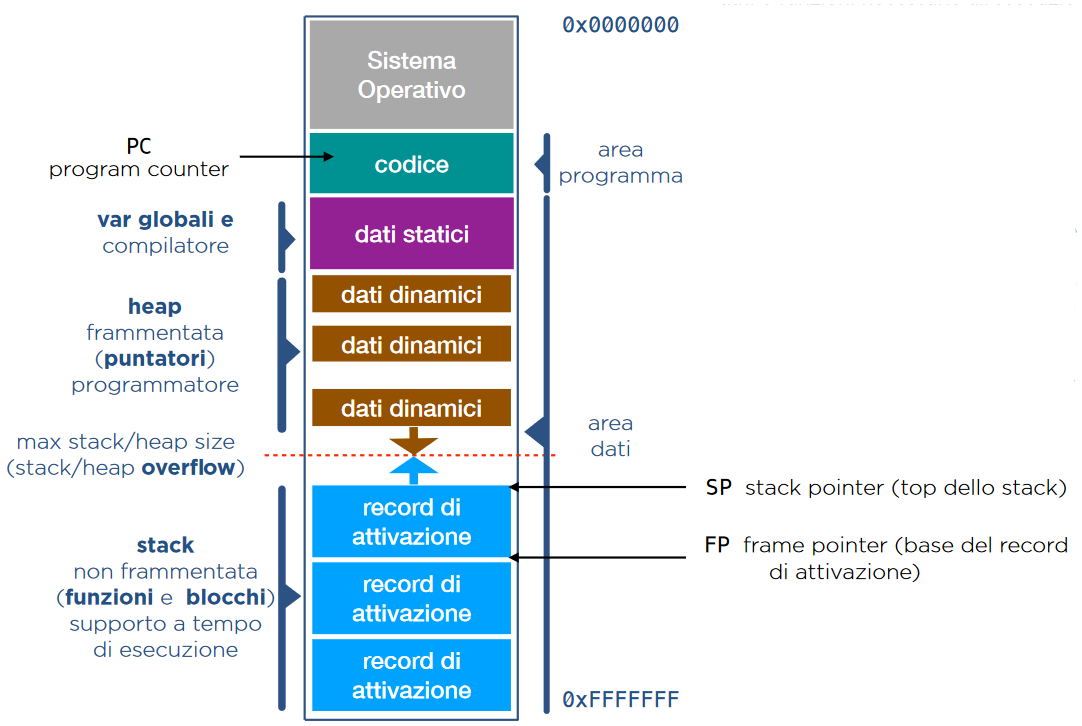
\includegraphics[width=13cm]{images/gestione-memoria.png}
	\caption{Gestione della memoria di un programma}
\end{figure}
\begin{note}
	Partiamo dal presupposto che un \textbf{blocco} sia considerato come una funzione senza parametri.
\end{note}
\newpage
\section{Ricorsione}
\begin{definition}[Ricorsione]
	A tempo di \textbf{compilazione}: una funzione usa il suo nome (chiama se stessa) nel suo corpo.
	A tempo di \textbf{esecuzione}: chiamate annidate della \textbf{stessa} funzione
\end{definition}
\noindent Una funzione ricorsiva è chiamata per risolvere un problema scomposto in:
\begin{itemize}
	\item \textbf{Caso base}: la funzione restituisce un valore
	\item \textbf{Passo ricorsivo}: la funzione viene chiamata su un problema analogo a quello iniziale ma di dimensioni minori, avvicinandosi al \emph{caso base}
\end{itemize}
Quando si  arriva al caso base viene effettuata una sequenza inversa di return statement, combinando i risultati parziali in quello finale.
\begin{example}[Fattoriale]
	Il fattoriale di un intero non negativo n è il prodotto
	degli interi positivi $<= n$ escluso lo $0$. Si indica con
	$n!$ e si impone per definizione $0! = 1$.
	\begin{equation}
		n! = \prod_{i=1}^{n} i=n*(n-1)*\ldots*1
	\end{equation}
	oppure definita in maniera ricorsiva:
	\begin{equation}
		n! = \begin{cases}
			1, \hspace{50px} n=0 \\
			n*(n-1)!, \hspace{6px} n>0
		\end{cases}
	\end{equation}
	In maniera programmatica possiamo scriverlo come:
	\begin{lstlisting}[language=Swift, caption=Fattoriale con ricorsione, mathescape=true]
		func F(var n: Int) -> Int {
			if (n-1) {
				return 1
			} else {
				return n * F(n-1)
			}
		}
	\end{lstlisting}
\end{example}

\subsection{Ricorsione e iterazione}
\begin{tabular} { |c|p{150px}|p{150px}|}
	\hline
	& \textbf{Ricorsione} & \textbf{Iterazione} \\
	\hline
	Controllo di terminazione & Condizione di ricorsione & Condizione di controllo nel loop \\
	\hline
	Ripetizioni & Chiamate ricorsive della funzione & Esecuzione ripetuta del corpo dell'iterazione \\
	\hline
	Convergenza alla terminazione & I passi ricorsivi riducono il problema al caso base & Il contatore si avvicina al valore di termine \\
	\hline
	Ripetizione infinita & Il passo ricorsivo non riduce il problema e non si avvicina al caso base & La condizione di controllo non è mai falsa \\
	\hline
\end{tabular}
\vspace{15pt}

\noindent Nella \emph{ricorsione}, al contrario dell'\emph{iterazione}, ogni chiamata alla funzione genera un nuovo record di attivazione contenente una nuova copia delle variabili e consumando lo stack di esecuzione. Questo può generare \textbf{overhead}.\\
In generale ogni problema \emph{ricorsivo} può essere anche scritto \emph{iterativamente}. È consigliato scriverlo ricorsivamente quando ciò facilita la lettura del problema stesso.
\newpage
\section{Condizioni}
\subsection{Condizioni su array}
Dato un array \textbf{a} di dimensione N, voglio verificare se la proprietà P vale per tutti gli elementi dell'array.
\begin{equation}
	\forall i \in [0, N).\mathcal{P}(a[i])
\end{equation}
\begin{example}
	Verifico che tutti gli elementi dell'array siano dispari.
	\begin{equation}
		\forall i \in [0, N).a[i]%2==1
	\end{equation}
	\begin{lstlisting}[language=C, caption=Verifica di proprietà su tutti gli elementi mathescape=true]
		int check_array_dispari(int a[], size_t dim) {
			int indice = 0;
			while (indice < dim && a[indice]%2 == 1){
				indice++;
			}
			if (indice == dim) {
				return 1;
			} else {
				return 0;
			}	
		}
	\end{lstlisting}
	Blocco lo scorrimento dell'array quando la proprietà \textbf{NON} viene soddisfatta almeno una volta.
\end{example}

\noindent
Se invece voglio verificare che la proprietà P valga per almeno un elemento:
\begin{equation}
	\exists i \in [0, N).\mathcal{P}(a[i])
\end{equation}
\begin{example}
	Verifico che almeno un elemento dell'array è uguale a 26.
	\begin{equation}
		\exists i \in [0, N).a[i]==26
	\end{equation}
	\begin{lstlisting}[language=C, caption=Verifica di proprietà su almeno un elemento, mathescape=true]
		int esiste_in_array(int a[], size_t dim, in n) {
			size_t indice = 0;
			_Bool trovato = 0;
			while (indice < dim && !trovato){
				if(a[indice] == n) {
					trovato = 1;	
				}
				indice++;
			}
			return trovato;
		}
	\end{lstlisting}
	Blocco lo scorrimento dell'array nel momento in cui trovo un elemento che soddisfa la proprietà, utilizzando un \textit{flag}.
\end{example}
\subsection{Condizioni su matrici}
Una \textbf{matrice} è un array di array. Può essere \textit{multidimensionale} $N \times M$ e voglio verificare se tutti i suoi elementi oppure solo uno di essi verificano una proprietà P.
\begin{equation}
	\forall i \in [0, N), \forall j \in [0,M).\mathcal{P}(a[i,j])
\end{equation}
\begin{equation}
	\exists i \in [0, N), \exists j \in [0,M).\mathcal{P}(a[i,j])
\end{equation}
\begin{definition}[Matrice quadrata]
	Una matrice è \textbf{quadrata} se a lo stesso numero di righe e di colonne. In questo caso per scorrerla si può usare un solo indice:
	\begin{equation}
		\exists i,j \in [0, N).\mathcal{P}(a[i,j])
	\end{equation}
\end{definition}

\begin{example}
	Verifico se tutti gli elementi della matrice sono positivi.
	\begin{equation}
		\forall i \in [0, N), \forall j \in [0, M) . a[i, j] > 0
	\end{equation}
	\begin{lstlisting}[language=C, caption=Verifica di proprietà su tutti gli elementi della matrice, mathescape=true]
		int check_matrice_pos(int a[][COL], size_t dim) {
			size_t row, col;
			row = col = 0;
			while (row < dim && a[row][col] > 0) {
				col = 0;
				while (col < COL && a[row][col] > 0) {
					col++;
				}
				if (col == COL) {
					row++;
				}
			}
			if (row == dim && col == COL) {
				return 1;
			}
			else {
				return 0;
			}
		}
	\end{lstlisting}
\end{example}
\begin{definition}[Matrice simmetrica]
	Una matrice è \textbf{simmetrica} se è quadrata e se le posizioni simmetriche rispetto alla diagonale principale contengono gli stessi elementi.
\end{definition}
\begin{definition}[Matrice triangolare]
	Una matrice è \textbf{triangolare} superiore o inferiore se le posizioni rispettivamente sopra o sotto la diagonale contengono tutti 0.
\end{definition}
\begin{definition}[Matrice tridiagonale]
	Una matrice \textbf{tridiagonale} \color{red} può \color{black} avere elementi non nulli solo sulla diagonale principale e la sua diagonale superiore ed inferiore.
\end{definition}

\subsection{Contare elementi che verificano una proprietà}
Dato un array \textbf{a} di dimensione $N$ per contare tutti gli elementi che verificano una proprietà $P$:
\begin{equation}
	\#\{i \lvert i\in [0, N-1] \land \mathcal{P}(a[i])\}
\end{equation}
Data invece una matrice \textbf{a} di dimensione $N \times M$:
\begin{equation}
	\#\{(i,j) \lvert i \in [0, N-1] \land j \in [0, M-1]\}
\end{equation}
\newpage
\section{Heap}
\begin{definition}[Heap binario]
	Un \textbf{albero} quasi completo.
\end{definition}
\begin{definition}[Albero binario completo]
	Un albero dove ogni nodo è foglia oppure ha due figli.
\end{definition}
\begin{definition}[Albero binario quasi completo]
	Se $h$ è l'altezza dell'albero, tutte le foglie hanno profondità $h$ oppure $h-1$. Tutti i nodi hanno $2$ figli eccetto al più $1$. Il nodo con un solo figlio, se esiste:
	\begin{itemize}
		\item ha profondità $h-1$
		\item tutti i nodi alla sua destra sono \textbf{foglie}
		\item e il suo unico figlio è un figlio \textbf{sinistro}
	\end{itemize}
\end{definition}

\begin{figure}[h]
	\begin{subfigure}{.5\textwidth}
		\centering
		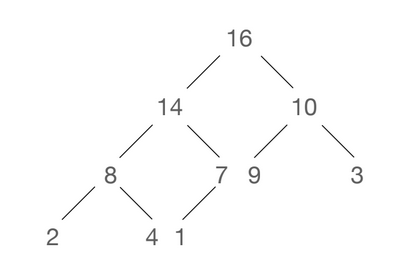
\includegraphics[width=6cm]{images/heap_tree.png}
		\caption{Albero binario quasi completo}
	\end{subfigure}
	\begin{subfigure}{.5\textwidth}
		\centering
		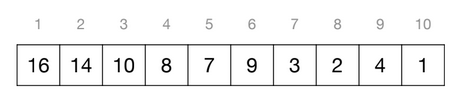
\includegraphics[width=6cm]{images/heap_array.png}
		\caption{Heap}
	\end{subfigure}
\end{figure}

\noindent
Di seguito alcune formule utili:
\begin{itemize}
	\item parent(i) = $\lfloor i/2 \rfloor$
	\item left(i) = $2i$
	\item right(i) = $2i+1$
\end{itemize}

\subsection{Max e min heap}
Dato un heap, se gli elementi di ogni sotto-albero sono più piccoli della radice del sotto-albero, allora abbiamo un \textbf{max-heap} e il massimo valore sarà memorizzato sempre nella radice.
\begin{equation}
	\forall i \neq 1, A[parent(i)] \geq A[i]
\end{equation}
Analogamente per il \textbf{min-heap} il minimo valore sarà nella radice.
\begin{equation}
	\forall i \neq 1, A[parent(i)] \leq A[i]
\end{equation}

\subsection{Proprietà}
\begin{itemize}
	\item \textbf{Proprietà 1}: un \textit{heap} di $n$ elementi ha altezza $\theta(\log{n})$, precisamente \color{red} $\lfloor \log{n} \rfloor$ \color{black}
	\item \textbf{Proprietà 2}: un \textit{heap} di $n$ elementi contiene \color{red} $\lceil n/2 \rceil$ \color{black} foglie
	\item \textbf{Proprietà 3}: un \textit{heap} di $n$ elementi ha al più \color{red} $\lceil n/2^{h+1} \rceil$ \color{black} nodi di altezza $h$, esattamente $\lceil n/2^{h+1} \rceil$ se è un albero \textit{bilanciato completo}
\end{itemize}
% !TeX spellcheck = it_IT
\newpage

\section{Algoritmi}
\subsection{Divide et impera}
È una tecnica di risoluzione di problemi che consiste in tre passi:
\begin{itemize}
	\item \textbf{Dividere} il problema in 2 o più sotto problemi identici ma di dimensione ridotta rispetto a quello originale
	\item \textbf{Risolvere} i sotto problemi \emph{ricorsivamente}
	\item \textbf{Combinare} le soluzioni dei sotto problemi per ottenere la soluzione del problema iniziale
\end{itemize}
\subsection{Ordinamento}
\begin{definition}[Algoritmo stabile]
	Un algoritmo di ordinamento si dice stabile quando preserva l'ordine iniziale tra due elementi con la stessa chiave.
\end{definition}
\subsubsection{Merge sort}
L'idea è di usare la tecnica precedentemente descritta del \textbf{Divide et Impera} e di spezzare l'array in due sotto-array di uguale dimensione, ordinarli e poi fonderli in uno unico. \\
La fusione verrà fatta confrontando i primi due elementi di ogni sotto-array, copiando il più piccolo nell'array finale, e proseguendo con il confronto del più grande con il successivo.
\begin{figure}[h]
	\begin{subfigure}{.5\textwidth}
		\centering
		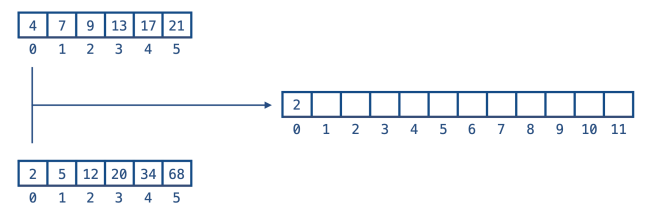
\includegraphics[width=8cm]{images/mergesort_1.png}
	\end{subfigure}
	\begin{subfigure}{.5\textwidth}
		\centering
		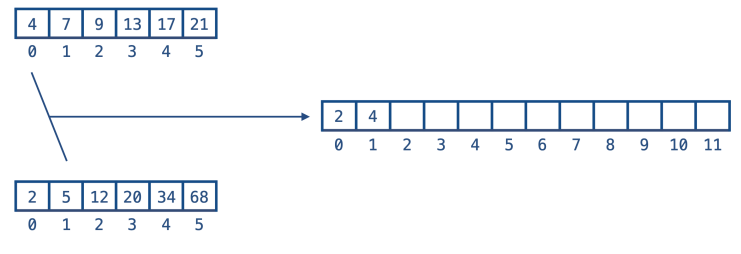
\includegraphics[width=8cm]{images/mergesort_2.png}
	\end{subfigure}
\end{figure}
\begin{figure}[h]
	\begin{subfigure}{.5\textwidth}
		\centering
		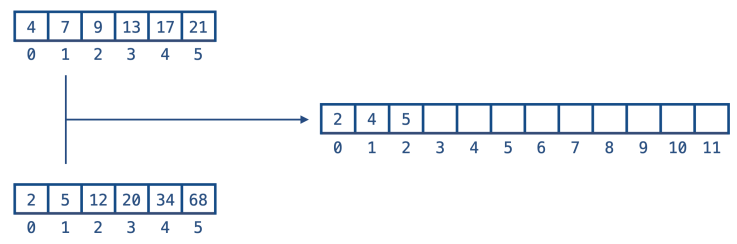
\includegraphics[width=8cm]{images/mergesort_3.png}
	\end{subfigure}
	\begin{subfigure}{.5\textwidth}
		\centering
		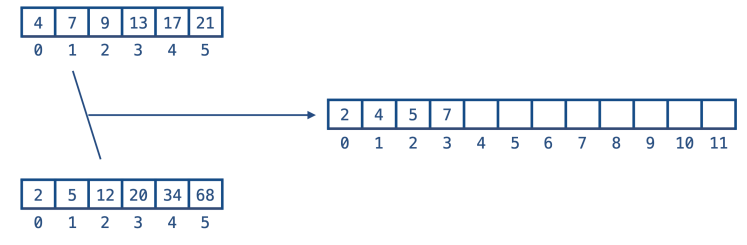
\includegraphics[width=8cm]{images/mergesort_4.png}
	\end{subfigure}
\end{figure}

\noindent Esempio di implementazione:

\begin{lstlisting}[language=C, caption=Algoritmo merge sort, mathescape=true]
	void merge_sort(int a[], size_t dim, char order) {
		sort(a, 0, dim-1, order);
	}

	void sort(int a[], size_t inizio, size_t fine, char order) {
		if ((fine - inizio) >= 1) {
			// Passo ricorsivo
			size_t centro1 = (inizio + fine)/2;
			zie_t centro2 = centro1 + 1;
			
			sort(a, inizio, centro1, order);
			sort(a, centro2, fine, order);
			
			merge(a, inizio, centro1, centro2, fine, order);
		}
		// Il caso base non serve, un array di un elemento e' ordinato
	}
	
	void merge(int a[], size_t sin, size_t centro1, size_t centro2, size_t dx, char order) {
		size_t sin i = sin;
		size_t dx_i = centro2;
		size_t fondi i = 0;
		int temp_a[dx - sin + 1];
		
		while (sin_i <= centro1 && dx_i <= dx) {
			switch (order) {
				case 'I':				
					if (a[sin_i] <= a[dx_i]) {
						temp_a[fondi_i++] = a[sin_i++];
					} else {
						temp_a[fondi_i++] = a[dx_i++];
					}
					break;
				default:
					if (a[sin_i] <= a[dx_i]) {
						temp_a[fondi_i++] = a[dx_i++];
					} else {
						temp_a[fondi_i++] = a[sin_i++];
					}
					break;
			}
		}
		
		// Se esaurisco il sotto-array sinistro
		if (sin_i == centro2) {
			while (dx_i <= dx) {
				temp_a[fondi_i++] = a[dx_i++];
			}
		} else {
			// Se esaurisco quello destro
			while (sin_i <= centro1) {
				temp_a[fondi_i++] = a[sin_i++];
			}
		}
	
		// Copio l'array temporaneo in quello originale
		for (size_t i = sin; i <= dx; i++) {
			a[i] = temp_a[i-sin];	
		}
	}
\end{lstlisting}

\subsubsection{Insertion sort}
\textbf{Proprietà}: al termine del passo j-esimo dell'algoritmo l'elemento j-esimo viene in inserito al posto giusto e i primi $j+1$ elementi sono ordinati.
\begin{lstlisting}[language=Javascript, caption=Algoritmo insertion sort, mathescape=true]
	insertionSort(A) =
	var j:Int = 0;
	var i:Int = 0;		$\Theta(1)$
	var k:int = 0;
	for (j=1; j<n; j++) {		$n-1$ volte
		k = A[j];
		i = j-1;		$\Theta(1)$ $n-1$ volte
		while(i >= 0 && A[i]>k) {
			A[i+1] = A[i];			$\Theta(1)$ $\sum\limits_{j=1}^{n-1} (t_j-1)$ volte
			i=i-1;
		}
		A[i+1] = k;		$\Theta(1)$ $n-1$ volte
	}
\end{lstlisting}

\begin{table}[h]
	\centering
	\begin{tabular}{ |c|c|c|c|c|c| }
		\hline
		0 & 1 & 2 & 3 & 4 & 5 \\
		\hline
		5 & 2 & 4 & 6 & 1 & 3 \\
		\hline 
		5 & 2 & 4 & 6 & 1 & 3 \\
		\hline 
		5 & 5 & 4 & 6 & 1 & 3 \\
		\hline 
		2 & 5 & 4 & 6 & 1 & 3 \\
		\hline 
		2 & 5 & 4 & 6 & 1 & 3 \\
		\hline 
		2 & 5 & 5 & 6 & 1 & 3 \\
		\hline 
		2 & 4 & 5 & 6 & 1 & 3 \\
		\hline 
		2 & 4 & 5 & 6 & 1 & 3 \\
		\hline 
		2 & 4 & 5 & 6 & 1 & 3 \\
		\hline 
	\end{tabular}
	\begin{tabular} { |c|c|c|c|}
		\hline
		j & i & k & while \\
		\hline
		0 & 0 & 0 & no \\
		\hline
		1 & 0 & 2 & si \\
		\hline
		1 & -1 & 2 & no \\
		\hline
		1 & -1 & 2 & no \\
		\hline
		2 & 1 & 4 & si \\
		\hline
		2 & 0 & 4 & no \\
		\hline
		2 & 0 & 4 & no \\
		\hline
		3 & 2 & 6 & no \\
		\hline
		3 & 2 & 6 & no \\
		\hline
	\end{tabular}
	\caption{Esempio di esecuzione}
\end{table}
\textbf{Complessità}:
\begin{align*}
	\sum\limits_{j=1}^{n-1} t_j
\end{align*}
\begin{itemize}
	\item Caso pessimo: l'array è ordinato decrescente e quindi ogni volta devo scalare l'elemento fino alla prima posizione. Abbiamo che $t_j = j$ e $\sum\limits_{j=1}^{n-1} j = \frac{n(n-1)}{2}$, quindi $O(n^2)$
	\item Caso migliore: l'array è ordinato crescente e quindi per ogni iterazione non entro nel while perché la condizione è falsa. Abbiamo $t_j = 1$ e $\sum\limits_{j=1}^{n-1} j = n-1$, quindi $O(n)$
	\item Caso medio: come il caso pessimo $O(n^2)$
\end{itemize}
\textbf{Correttezza}:
\begin{itemize}
	\item dimostro l'\textbf{invariante di ciclo} per assicurarmi che la mia proprietà venga mantenuta durante tutta l'esecuzione. Lo faccio tramite \emph{induzione}:
	\begin{itemize}
		\item Caso base: per $j=1$
		\item Hp induttiva: per $j=n'$
		\item Passo induttivo: dimostro che vale anche per $j=n'+1$
	\end{itemize}
	\item verifico la \textbf{terminazione}: il \emph{for} è eseguito esattamente $n-1$ volte e il \emph{while} al più $j-1$ volte, quindi tutte le iterazioni sono finite e l'algoritmo termina.
\end{itemize}
\textbf{Memoria impiegata}: ordina in loco quindi non usa memoria aggiuntiva.

\subsubsection{Selection sort}
\textbf{Proprietà}: al termine del passo j-esimo dell'algoritmo i primi $j+1$ elementi di A sono ordinati e contengono i $j+1$ elementi più piccoli di A.
%TODO Calcolo della complessità non corretto
\begin{lstlisting}[language=Javascript, caption=Algoritmo selection sort, mathescape=true]
	insertionSort(A) =
	var j:Int = 0;
	var i:Int = 0;		$\Theta(1)$
	var min:int = 0;
	for (i=0; i<n-1; i++) {		$n-1$ volte
		min = i;		$\Theta(1)$ $n-1$ volte
		for(j=i+1; j<n; j++) {
			if A[j] < A[min] {min = j};			$\Theta(1)$ $\sum\limits_{j=1}^{n-1} (t_j-1)$ volte
		}
		swap(A[i],A[min]);		$\Theta(1)$ $n-1$ volte
	}
\end{lstlisting}
\begin{table}[h]
	\centering
	\begin{tabular}{ |c|c|c|c|c|c| }
		\hline
		0 & 1 & 2 & 3 & 4 & 5 \\
		\hline
		5 & 2 & 4 & 6 & 1 & 3 \\
		\hline 
		1 & 2 & 4 & 6 & 5 & 3 \\
		\hline 
		1 & 2 & 4 & 6 & 5 & 3 \\
		\hline 
		1 & 2 & 3 & 6 & 5 & 4 \\
		\hline 
		1 & 2 & 3 & 4 & 5 & 6 \\
		\hline 
		1 & 2 & 3 & 4 & 5 & 6 \\
		\hline
	\end{tabular}
	\begin{tabular} { |c|c|c|}
		\hline
		j & i & min \\
		\hline
		0 & 0 & 0 \\
		\hline
		1 & 0 & 4 \\
		\hline
		2 & 1 & 1 \\
		\hline
		3 & 2 & 5 \\
		\hline
		4 & 3 & 3 \\
		\hline
		5 & 4 & 4 \\
		\hline
	\end{tabular}
	\caption{Esempio di esecuzione}
\end{table}
\textbf{Complessità}
%TODO Inserisci il calcolo della complessità
\begin{align*}
	\sum\limits_{j=1}^{n-1} j = \frac{n(n-1)}{2} \in O(n^2)
\end{align*}
\begin{itemize}
	\item Caso pessimo: $O(n^2)$
	\item Caso migliore: $O(n^2)$
	\item Caso medio: $O(n^2)$
\end{itemize}
\textbf{Correttezza}:
\begin{itemize}
	\item dimostro l'\textbf{invariante di ciclo} per assicurarmi che la mia proprietà venga mantenuta durante tutta l'esecuzione. Sempre tramite induzione.
	\item verifico la \textbf{terminazione} in maniera analoga all'insertion sort.
\end{itemize}
\textbf{Memoria impiegata}: ordina in loco quindi non usa memoria aggiuntiva.

\subsubsection{Bubble sort}
Questo algoritmo scorre l'array e, a coppie, ordina gli elementi facendo più passate. Il nome \emph{bubble} deriva dal fatto che ad ogni passata i numeri più grandi (o piccoli) si spostano verso la fine dell'array come le bolle d'aria salgono a galla.
\begin{lstlisting}[language=C, caption=Algoritmo bubble sort, mathescape=true]
	void bubble_sort (int a[], size_t dim, char order) {
		int temp;
		for (unsigned int passate = 0; passate < dim; passate++) {
			for (size_t i=0; i < (dim - 1); i++) {
				switch (order) {
					case 'I':
						if (a[i] > a[i+1]) {
							temp = a[i];
							a[i] = a[i+1];
							a[i+1] = temp;
						}
						break;
					default:
						if (a[i] < a[i+1]) {
							temp = a[i];
							a[i] = a[i+1];
							a[i+1] = temp;
							 break;
						}
				}
			}
		}
	}
\end{lstlisting}
\textbf{Complessità}\\
Il primo \emph{for} esegue $n$ cicli e quello interno ne esegue $n-1$. Di conseguenza la complessità è $n\cdot (n-1)$, ovvero $\mathbf{n^2}$.
\subsection{Linear sort}
Gli algoritmi di ordinamento di questo tipo sfruttano il fatto che l'array da ordinare abbia determinate proprietà.
\begin{example}
	Dato un array $A$ di $n$ interi compresi tra $1$ e $k$:
	\begin{align*}
		\forall 0 < j \leq n . A[j] \in [1, \ldots, k]
	\end{align*}
	\begin{lstlisting}[language=Javascript, caption=Algoritmo linear sort, mathescape=true]
		linearSort(A:[Int], B:[Int], k:Int) -> Void {
			// Inizializzo un array che tiene conto dei numeri da 1 a k
			for (var i:Int = 1; i<=k; i++) C[i] = 0;	$\Theta(k)$
			
			var j:Int = 1;
			// Conto quante volte compare ogni numero nell'array originale
			for (j=1; j<=n; j++) C[A[j]] += 1;	$\Theta(n)$
				
			j=1;
			var z:Int = 1;
			// Dispongo ogni numero nell'array finale in ordine sapendo quante volte compare
			for (z=1; z <= k; z++) {	$\Theta(k)$
				for (var v:Int = 0; v < C[z]; v++) {	$\Theta(n)$
					B[j] = z;
					j++;	
				}	
			}	
		}
	\end{lstlisting}
	\textbf{Complessità}\\
	In questo caso la complessità è $\Theta(n + k)$ e si usa quando $k \in O(n)$.
\end{example}
\subsubsection{Radix sort}
Questo algoritmo funziona in maniera simile a come il cervello umano ordina gruppi di numeri: si ordinano (tramite un algoritmo di ordinamento \textbf{stabile} prima le cifre delle migliaia, poi quelle delle centinaia, quelle delle decine ed infine le unità. Notiamo però che il risultato NON è corretto.
\begin{table}[h]
	\centering
	\begin{tabular}{ccccc}
		\textbf{1}094 & \textbf{9}86 & 10\textbf{9}4 & 12\textbf{5} & 1120 \\
		986 & \textbf{2}34 & 1\textbf{2}5 & 112\textbf{0} & 234 \\
		234 & \textbf{1}25 & 11\textbf{2}0 & 23\textbf{4} & 1094 \\
		125 & 1\textbf{0}94 & 2\textbf{3}4 & 98\textbf{6} & 125 \\
		\textbf{1}120 & 1\textbf{1}20 & 9\textbf{8}6 & 109\textbf{4} & 986
	\end{tabular}
\end{table}
\\
Per farlo funzionare dobbiamo ordinare le cifre partendo da quelle meno significative, quindi dalle unità.
\begin{table}[h]
	\centering
	\begin{tabular}{ccccc}
		109\textbf{4} & 11\textbf{2}0 & 1\textbf{1}20& \textbf{1}094 & 125 \\
		98\textbf{6} & 10\textbf{9}4 & \textbf{1}25 & \textbf{1}120 & 234 \\
		23\textbf{4} & 2\textbf{3}4 & \textbf{2}34 & 125 & 986 \\
		12\textbf{5} & 1\textbf{2}5 & \textbf{9}86 & 234 & 1094 \\
		112\textbf{0} & 9\textbf{8}6 & 1\textbf{0}94 & 986 & 1120
	\end{tabular}
\end{table}
\section{Complessità}
\subsection{Limiti inferiori}
\subsubsection{Complessità di un problema}
Per determinare il limite inferiore di un problema al caso pessimo, analizzo le seguenti cose:
\begin{itemize}
	\item \textbf{Dimensione dei dati}: Se la soluzione di un problema richiede l'esame di tutti i dati in input, allora $\Omega(n)$ è un limite inferiore. \emph{E.g. sommare tutti gli elementi di un array.}
	\item \textbf{Eventi contabili}: se la soluzione di un problema richiede la ripetizione di un certo evento, allora il numero di volte che l'evento si ripete (moltiplicato per il suo costo) è un limite inferiore.
	\item \textbf{Alberi di decisione}: sono alberi in cui
	\begin{itemize}
		\item ogni nodo non foglia effettua un test su un attributo
		\item ogni arco uscente da un nodo è un possibile valore dell'attributo
		\item ogni nodo foglia assegna una classificazione
	\end{itemize}
	Si applica a problemi risolubili attraverso sequenze di decisioni che via via riducono lo spazio delle soluzioni.
	%TODO inserire immagine di albero di decisione
	\begin{note}
		Alcune formule importanti per gli alberi:
		%TODO Inserisci formule
	\end{note}
	%TODO Esempio con ricerca binaria
\end{itemize}

\subsubsection{Ordinamento}
\subsubsection{Insertion sort}
\textbf{Proprietà}: al termine del passo j-esimo dell'algoritmo l'elemento j-esimo viene in inserito al posto giusto e i primi $j+1$ elementi sono ordinati.
\begin{lstlisting}[language=Javascript, caption=Algoritmo insertion sort, mathescape=true]
	insertionSort(A) =
	var j:Int = 0;
	var i:Int = 0;		$\Theta(1)$
	var k:int = 0;
	for (j=1; j<n; j++) {		$n-1$ volte
		k = A[j];
		i = j-1;		$\Theta(1)$ $n-1$ volte
		while(i >= 0 && A[i]>k) {
			A[i+1] = A[i];			$\Theta(1)$ $\sum\limits_{j=1}^{n-1} (t_j-1)$ volte
			i=i-1;
		}
		A[i+1] = k;		$\Theta(1)$ $n-1$ volte
	}
\end{lstlisting}
\begin{table}[h]
	\begin{tabular}{ |c|c|c|c|c|c| }
		\hline
		0 & 1 & 2 & 3 & 4 & 5 \\
		\hline
		5 & 2 & 4 & 6 & 1 & 3 \\
		\hline 
		5 & 2 & 4 & 6 & 1 & 3 \\
		\hline 
		5 & 5 & 4 & 6 & 1 & 3 \\
		\hline 
		2 & 5 & 4 & 6 & 1 & 3 \\
		\hline 
		2 & 5 & 4 & 6 & 1 & 3 \\
		\hline 
		2 & 5 & 5 & 6 & 1 & 3 \\
		\hline 
		2 & 4 & 5 & 6 & 1 & 3 \\
		\hline 
		2 & 4 & 5 & 6 & 1 & 3 \\
		\hline 
		2 & 4 & 5 & 6 & 1 & 3 \\
		\hline 
	\end{tabular}
	\begin{tabular} { |c|c|c|c|}
		\hline
		j & i & k & while \\
		\hline
		0 & 0 & 0 & no \\
		\hline
		1 & 0 & 2 & si \\
		\hline
		1 & -1 & 2 & no \\
		\hline
		1 & -1 & 2 & no \\
		\hline
		2 & 1 & 4 & si \\
		\hline
		2 & 0 & 4 & no \\
		\hline
		2 & 0 & 4 & no \\
		\hline
		3 & 2 & 6 & no \\
		\hline
		3 & 2 & 6 & no \\
		\hline
	\end{tabular}
	\caption{Esempio di esecuzione}
\end{table}
\textbf{Complessità} bla bla bla\\ %TODO Inserisci il calcolo della complessità
\textbf{Correttezza}:
\begin{itemize}
	\item dimostro l'\textbf{invariante di ciclo} per assicurarmi che la mia proprietà venga mantenuta durante tutta l'esecuzione. Lo faccio tramite \emph{induzione}:
	\begin{itemize}
		\item Caso base: per $j=1$
		\item Hp induttiva: per $j=n'$
		\item Passo induttivo: dimostro che vale anche per $j=n'+1$
	\end{itemize}
	\item verifico la \textbf{terminazione}: il \emph{for} è eseguito esattamente $n-1$ volte e il \emph{while} al più $j-1$ volte, quindi tutte le iterazioni sono finite e l'algoritmo termina.
\end{itemize}
\textbf{Memoria impiegata}: ordina in loco quindi non usa memoria aggiuntiva.

\subsubsection{Selection sort}
\textbf{Proprietà}: al termine del passo j-esimo dell'algoritmo i primi $j+1$ elementi di A sono ordinati e contengono i $j+1$ elementi più piccoli di A.
\begin{lstlisting}[language=Javascript, caption=Algoritmo selection sort, mathescape=true]
	insertionSort(A) =
	var j:Int = 0;
	var i:Int = 0;		$\Theta(1)$
	var min:int = 0;
	for (i=0; i<n-1; i++) {		$n-1$ volte
		min = i;		$\Theta(1)$ $n-1$ volte
		for(j=i+1; j<n; j++) {
			if A[j] < A[min] {min = j};			$\Theta(1)$ $\sum\limits_{j=1}^{n-1} (t_j-1)$ volte
		}
		swap(A[i],A[min]);		$\Theta(1)$ $n-1$ volte
	}
\end{lstlisting}
\begin{table}[h]
	\begin{tabular}{ |c|c|c|c|c|c| }
		\hline
		0 & 1 & 2 & 3 & 4 & 5 \\
		\hline
		5 & 2 & 4 & 6 & 1 & 3 \\
		\hline 
		1 & 2 & 4 & 6 & 5 & 3 \\
		\hline 
		1 & 2 & 4 & 6 & 5 & 3 \\
		\hline 
		1 & 2 & 3 & 6 & 5 & 4 \\
		\hline 
		1 & 2 & 3 & 4 & 5 & 6 \\
		\hline 
		1 & 2 & 3 & 4 & 5 & 6 \\
		\hline
	\end{tabular}
	\begin{tabular} { |c|c|c|}
		\hline
		j & i & min \\
		\hline
		0 & 0 & 0 \\
		\hline
		1 & 0 & 4 \\
		\hline
		2 & 1 & 1 \\
		\hline
		3 & 2 & 5 \\
		\hline
		4 & 3 & 3 \\
		\hline
		5 & 4 & 4 \\
		\hline
	\end{tabular}
	\caption{Esempio di esecuzione}
\end{table}
\textbf{Complessità}
%TODO Inserisci il calcolo della complessità
\begin{equation}
	\sum\limits_{j=1}^{n-1} j = \frac{n(n-1)}{2} \in O(n^2)
\end{equation}
\begin{itemize}
	\item Caso pessimo: $O(n^2)$
	\item Caso migliore: $O(n^2)$
	\item Caso medio: $O(n^2)$
\end{itemize}
\textbf{Correttezza}:
\begin{itemize}
	\item dimostro l'\textbf{invariante di ciclo} per assicurarmi che la mia proprietà venga mantenuta durante tutta l'esecuzione. Sempre tramite induzione.
	\item verifico la \textbf{terminazione} in maniera analoga all'insertion sort.
\end{itemize}
\textbf{Memoria impiegata}: ordina in loco quindi non usa memoria aggiuntiva.
% !TeX spellcheck = it_IT
\newpage
\section{Liste}
Una \textbf{struct} (struttura) \textbf{autoreferenziale} ha un membro puntatore che punta a una struttura dello stesso tipo, chiamato \textbf{link}, e che serve a creare una \emph{catena} (lista) di nodi collegati tra loro.
\begin{lstlisting}[language=C, caption=Esempio di una struct]
	struct nodo {
		int dato;
		struct nodo *nextPtr;
	} n1, n2, n3;
\end{lstlisting}

\begin{definition}[Struttura dinamica]
	È una struttura dati che può \textbf{variare} la sua dimensione a tempo di esecuzione, aumentando e diminuendo. Alcuni esempi sono proprio le \textbf{liste}, oltre che le pile, le code e gli alberi binari.
\end{definition}

\begin{note}
	L'ultimo nodo di una lista conterrà nel link \textbf{null}.
\end{note}

\subsection{Confronto tra liste e array}
\begin{table}[!h]
	\centering
	\begin{tabular}{|p{150px}|p{150px}|}
		\hline
		\textbf{Liste} & \textbf{Array} \\
		\hline
		Contiene sequenze di dati & Contiene sequenze di dati \\ 
		\hline
		Create dinamicamente a tempo di esecuzione e la dimensione non può essere prevista a tempo di compilazione & Creati staticamente a tempo di esecuzione e la dimensione deve essere calcolabile a tempo di compilazione \\
		\hline
		La dimensione è variabile &  La dimensione è costante e tutti gli elementi sono allocati a tempo di definizione\\
		\hline
		Diventa piena solo quando termina la memoria disponibile nell'heap & Diventa pieno quando sono pieni tutti gli elementi \\
		\hline
		Non sono memorizzate in celle contigue & Sono in celle contigue \\
		\hline
		Possono essere manipolate senza spostare elementi & Per manipolarli bisogna spostare gli elementi \\
		\hline
	\end{tabular}
\end{table}

\subsection{Operazioni sulle liste}
\subsubsection{Insert}
Viene codificata come segue:
\begin{lstlisting}[language=C, caption=Inserimento in una lista]
	void insert(NodoPtr *lPtr, int val) {
		// Alloco nuovo nodo
		NodoPtr nuovoPtr = malloc(sizeof(Nodo));
		if (nuovoPtr != NULL) {
			// Inizializzo nodo
			nuovoPtr->dato = val;
			nuovoPtr->prossimoPtr = NULL;
			NodoPtr precedentePtr = NULL;
			NodoPtr correntePtr = *lPtr;
			while (correntePtr != NULL && val > correntePtr->dato) {
				precedentePtr = correntePtr;
				correntePtr = correntePtr->prossimoPtr;
			}
			if (precedentePtr == NULL) {
				// Inserimento all'inizio della lista
				nuovoPtr->prossimoPtr = *lPtr;
				*lPtr = nuovoPtr;
			}
			else {
				// Inserimento tra due nodi
				precedentePtr->prossimoPtr = nuovoPtr;
				nuovoPtr->prossimoPtr = correntePtr;
			}
		}
		else {
			puts("Memoria esaurita");
		}
	}
\end{lstlisting}

\subsubsection{Delete}
Viene codificata come segue:
\begin{lstlisting}[language=C, caption=Cancellazione in una lista]
void delete(NodoPtr *lPtr, int val) {
	if (*lPtr != NULL) {
		if (val == (*lPtr)->dato) {
			NodoPtr tempPtr = *lPtr;
			*lPtr = (*lPtr)->prossimoPtr;
			free(tempPtr);
		}
		else {
			NodoPtr precedentePtr = *lPtr;
			NodoPtr correntePtr = (*lPtr)->prossimoPtr;
			while (correntePtr != NULL && correntePtr->dato != val) {
				precedentePtr = correntePtr;
				correntePtr = correntePtr->prossimoPtr;
			}
			if (correntePtr != NULL) {
				NodoPtr tempPtr = correntePtr;
				precedentePtr->prossimoPtr = correntePtr->prossimoPtr;
				free(tempPtr);
			}
		}
	}
}
\end{lstlisting}

\subsubsection{Verifica se è vuota}
\begin{lstlisting}[language=C, caption=Verificare se la lista è vuota]
int is_empty(NodoPtr lPtr) {
	return lPtr == NULL;
}
\end{lstlisting}

\subsection{Liste particolari}
\subsubsection{Pile}
\begin{definition}
	Una \textbf{pila} è una lista in cui inserimenti e cancellazioni possono essere fatte solo sulla testa della lista (politica \textbf{LIFO}).
\end{definition}
Le operazioni che possono essere eseguite sulle pile sono:
\begin{itemize}
	\item \textbf{Push}: inserimento di un nuovo nodo in testa
	\begin{lstlisting}[language=C]
		void push(NodoPtr *topPtr, int val) {
			// alloco nuovo nodo
			NodoPtr nuovoPtr = malloc(sizeof(Nodo));
			if (nuovoPtr != NULL) { // Spazio disponibile
				// inizializzo nodo
				nuovoPtr->dato = val;
				nuovoPtr->prossimoPtr = *topPtr;
				*topPtr = nuovoPtr;
			}
			else {
				puts("Memoria esaurita");
			}
		}
	\end{lstlisting}
	\item  \textbf{Pop}: cancellazione di un elemento in testa
	\begin{lstlisting}[language=C]
		int pop(NodoPtr *topPtr) {
			int val = (*topPtr)->dato;
			NodoPtr tempPtr = *topPtr;
			*topPtr = (*topPtr)->prossimoPtr;
			free(tempPtr);
			return val;
		}
	\end{lstlisting}
	\item \textbf{is\_empty}, \textbf{stampa\_pila}
\end{itemize}

\subsubsection{Code}
\begin{definition}
	Una \textbf{pila} è una lista in cui inserimenti e cancellazioni possono essere fatte solo alla fine della lista (politica \textbf{FIFO}).
\end{definition}
Le operazioni che possono essere eseguite sulle pile sono:
\begin{itemize}
	\item \textbf{Enqueue}: inserimento di un nuovo nodo alla fine della coda
	\begin{lstlisting}[language=C]
		void enqueue(NodoPtr *testaPtr, NodoPtr * codaPtr, int val) {
			// alloco nuovo nodo
			NodoPtr nuovoPtr = malloc(sizeof(Nodo));
			if (nuovoPtr != NULL) { // Spazio disponibile
				// inizializzo nodo
				nuovoPtr->dato = val;
				nuovoPtr->prossimoPtr = NULL;
				if (is_empty(*testaPtr)) {
					*testaPtr = nuovoPtr;
				}
				else {
					(*codaPtr)->prossimoPtr = nuovoPtr;
					*codaPtr = nuovoPtr;
				}
			}
			else {
				puts("Memoria esaurita");
			}
		}
	\end{lstlisting}
	\item  \textbf{Dequeue}: cancellazione di un elemento in testa
	\begin{lstlisting}[language=C]
		int dequeue(NodoPtr *testaPtr, NodoPtr * codaPtr) {
			int val = (*testaPtr)->dato;
			NodoPtr tempPtr = *testaPtr;
			*testaPtr = (*testaPtr)->prossimoPtr;	
			if (*testaPtr == NULL) {
				*codaPtr = NULL;
			}
			free(tempPtr);
			return val;
		}
	\end{lstlisting}
	\item \textbf{is\_empty}, \textbf{stampa\_coda}
\end{itemize}
% !TeX spellcheck = it_IT
\newpage
\section{Dizionari}
\begin{definition}
	Un dizionario è una \textbf{struttura dati astratta} e consiste in una collezione di \textbf{coppie} della forma:
	\begin{itemize}
		\item \textbf{Chiave}: è il meccanismo di accesso all'elemento ed è \textbf{univoca} nella collazione
		\item \textbf{Elemento}:  è un qualsiasi tipo
	\end{itemize} 
\end{definition}
Le operazioni che possono essere eseguite sui dizionari sono \emph{inserimento}, \emph{ricerca} e \emph{cancellazione}.
\subsection{Indirizzamento diretto}
Ogni elemento del dizionario viene mappato con una chiave estratta da un determinato universo $U$ e che corrisponde alla posizione nell'array dove viene inserito. \\
La complessità di questa tecnica è $O(1)$ per tutte e tre le operazioni possibili sui dizionari. Il problema si presenta quando le chiavi usate $N$ sono molto minori dell'universo iniziale $U$ e abbiamo quindi che $\frac{N}{U} < 1$ con un conseguente \textbf{spreco di spazio di memoria} in quanto lo spazio nell'array dovrà comunque essere allocato.
\subsection{Chaining}
Un modo per evitare i problemi dell'\emph{indirizzamento diretto} è utilizzando un array più piccolo dell'universo possibile di chiavi. Questo ovviamente causa situazioni in cui c'è un \textbf{conflitto} perché due o più elementi voglio utilizzare la stessa chiave. Viene quindi creata una \textbf{lista} di elementi associata alla posizione in cui si è creato il conflitto e ogni nuovo elemento che vuole inserirsi lì verrà messo sulla testa della lista. \\
Per capire ogni elemento a quale chiave deve essere associato si utilizza una \textbf{funzione di hash} che deve essere definita in modo da ridurre il numero di collisioni e da generare sempre lo stesso indice per la stessa chiave.
%TODO Inserisci immagini
\subsection{Open addressing}
I conflitti di indirizzo vengono risolti cercando la prima posizione libera. Questo processo di ricerca viene chiamato \textbf{probing}. Questa operazione può avvenire in diversi modi:
\begin{itemize}
	\item \emph{Lineare}: vado alla posizione successiva
	\item \emph{Quadratico}: uso una funzione quadratica
	\item \emph{Doppio hash}: utilizzo la funzione hash per cercare la posizione successiva
\end{itemize}
\begin{example}
	Esempio di esecuzione di \emph{probing}:
	\begin{gather*}
		probe(0) \longrightarrow h(i) \\
		probe(1) \longrightarrow (h(i) + f(1))\\
		\vdots \\
		probe(j) \longrightarrow (h(i) + f(j))\\
		\vdots \\
		probe(m-1) \longrightarrow Fail\\
	\end{gather*}
\end{example}

\begin{example}
	Esempio di \emph{probing lineare}.
\end{example}
\begin{observation}
	Il problema che nasce dell'open addressing lineare è il \textbf{clustering primario}. Quando infatti si verifica una collisione, viene riempita una cella di memoria nelle vicinanze, aumentando così il rischio di collisione e aumentando il tempo necessario per la ricerca. \\ Questo avviene perché la \emph{probabilità} che uno slot preceduto da slot pieni sia riempito è pari a $\frac{i + 1}{m}$.
\end{observation}
\begin{observation}
	Il problema che deriva dall'utilizzo di open addressing quadratico è il \textbf{clustering secondario}. Infatti in questo caso se due chiavi hanno la stessa posizione iniziale la loro sequenza di tentativi sarà la stessa.
\end{observation}
% !TeX spellcheck = it_IT
\newpage
\section{Alberi}
%TODO Integrare robe ovvie sugli alberi
\subsection{Rappresentazione}
\subsubsection{Array}
Per rappresentare un albero \emph{binario} di profondità $d$ possiamo utilizzare un \textbf{array} di dimensione $2^{d+1}-1$. Questa scelta può portare a dei vantaggi e svantaggi:
\begin{itemize}
	\item \textbf{Vantaggi}:
	\begin{itemize}
		\item Accesso diretto ai nodi
	\end{itemize}
	\item \textbf{Svantaggi}:
	\begin{itemize}
		\item L'\emph{altezza} dell'albero deve essere nota
		\item Spreco di memoria
		\item \emph{Inserimento} e \emph{cancellazione} sono operazioni complicate
	\end{itemize}
\end{itemize}
Per questi motivi gli array si usano raramente per la rappresentazione di alberi.
\subsubsection{Liste}
Il modo più usato per la rappresentazione di alberi è quello delle \textbf{liste}, codificandoli come segue:
\begin{lstlisting}[language=C, caption=Alberi con liste, mathescape=true]
	struct node {
		int data;
		struct node *left;
		struct node *right;
	}
\end{lstlisting}
Questa scelta ci porta a vantaggi e svantaggi:
\begin{itemize}
	\item \textbf{Vantaggi}:
	\begin{itemize}
		\item L'\emph{altezza} dell'albero non deve essere nota
		\item Nessuno spreco di memoria
		\item \emph{Inserimento} e \emph{cancellazione} sono operazioni facili
	\end{itemize}
	\item \textbf{Svantaggi}:
	\begin{itemize}
		\item Mancanza di accesso diretto ai nodi
		\item Memoria aggiuntiva per memorizzare figlio destro e sinistro
	\end{itemize}
\end{itemize}

\subsection{Visitare}
Possiamo effettuare l'operazione di \textbf{visita} su un albero binario in tre modi diversi. Tutti questi algoritmi avranno \textbf{complessità} $O(n)$.
\subsubsection{Anticipata}
\begin{lstlisting}[language=C, caption=Alberi con liste, mathescape=true]
	Anticipata(x):
		if x != NULL
			print(x.key)
			Anticipata(x.left)
			Anticipata(x.right)
\end{lstlisting}
\begin{example}
	%TODO Da finire
\end{example}
\subsubsection{Posticipata}
\begin{lstlisting}[language=C, caption=Alberi con liste, mathescape=true]
	Posticipata(x):
		if x != NULL
			Posticipata(x.left)
			Posticipata(x.right)
			print(x.key)
\end{lstlisting}
\begin{example}
	%TODO Da finire
\end{example}
\subsubsection{Simmetrica}
\begin{lstlisting}[language=C, caption=Alberi con liste, mathescape=true]
	Simmetrica(x):
		if x != NULL
			Simmetrica(x.left)
			print(x.key)
			Simmetrica(x.right)
\end{lstlisting}
\begin{example}
	%TODO Da finire
\end{example}
\subsection{Albero binario di ricerca}
Un caso particolare di albero binario è un albero binario di ricerca. Questo rispecchia le seguenti proprietà, dato un nodo $x$, applicate ricorsivamente:
\begin{itemize}
	\item $x.left.key \leq x.key$, ovvero tutti i nodi alla sinistra sono i minori di $x$
	\item $x.right.key \geq x.key$, ovvero tutti i nodi alla destra sono i maggiori di $x$
\end{itemize}
\begin{note}
	Per effettuare la stampa \textbf{ordinata} degli elementi dobbiamo utilizzare la visita \textbf{simmetrica}.
\end{note}
\subsubsection{Ricerca}
Algoritmo ricorsivo per la ricerca di un elemento:
\begin{lstlisting}[language=C, caption=Ricerca ricorsiva, mathescape=true]
	RicercaABR_R(x, k)
		if x == NULL OR k == x.key
			return x
		if k < x.key
			return RicercaABR_R(x.left, k)
		else return RicercaABR_R(x.right, k)
\end{lstlisting}
Algoritmi per la ricerca del valore minimo e massimo di un albero:
\begin{lstlisting}[language=C, caption=Ricerca del minimo, mathescape=true]
	RicercaMIN_I(x)
		while x.left != NULL
			x = x.left
		return x
\end{lstlisting}
\begin{lstlisting}[language=C, caption=Ricerca del massimo, mathescape=true]
	RicercaMAX_I(x)
		while x.right != NULL
			x = x.right
		return x
\end{lstlisting}
\newpage
\section{Grafi}
\subsection{Grafo orientato}
\begin{definition}[Grafo orientato]
Un grafo orientato è una relazione $E: V \leftrightarrow V$ su un insieme finito $V$. In un grafo $V$ è l'insieme di nodi o vertici, $E$ è l'insieme di archi o lati. Chiamiamo $G$ (o $G^1$, $G_1$, $G_2$) e scriviamo $G = (V,E)$
\end{definition}
 

\begin{example}\label{esempio-grafo-1}
    Qui di seguito un esempio di un grafo:
\end{example}
 
\hspace{-15pt}Dati i due insiemi $V$ e $E$:\\\\
$V = \{0,1,2,3,4,5\}$ \\
$E = \{(0,0), (0,1), (0,5), (1,3), (1,5), (2,1), (3,4), (3,5), (5,3), (5,4)\}$\\ \\
\begin{wrapfigure}[4]{r}{5cm}
    \vspace{-100pt}
    \centering
    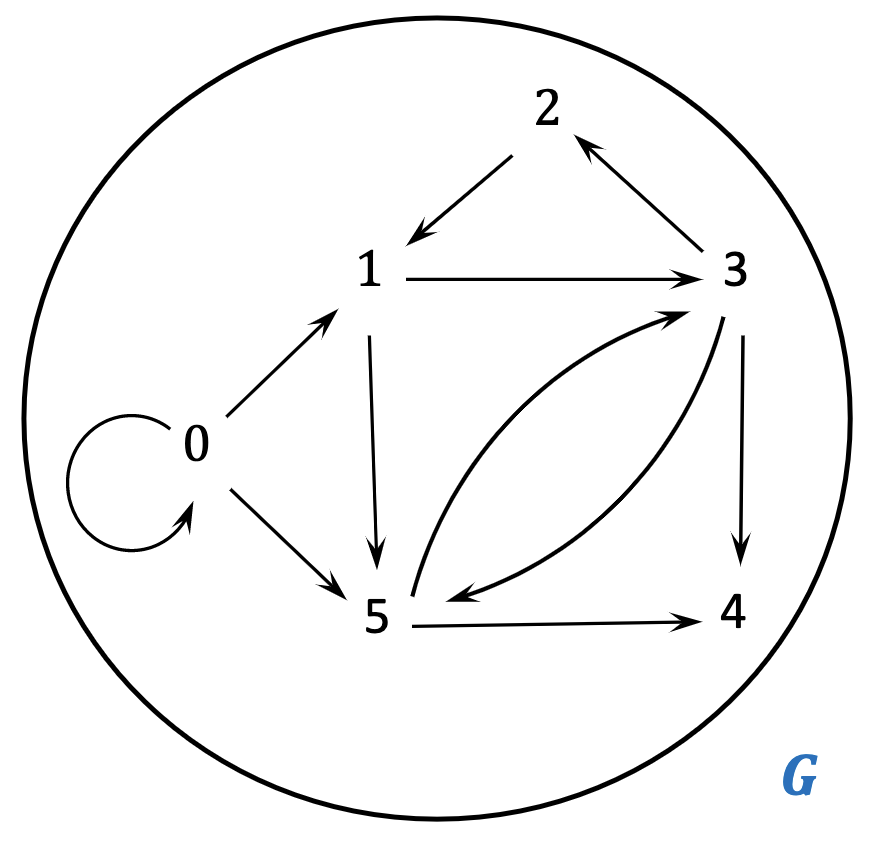
\includegraphics[width=3.7cm]{images/esempio-grafo.png}
    \vspace{-5pt}
    \caption{Grafo G}
    \label{fig:esempio-grafo}
\end{wrapfigure}
Quello rappresentato nell'immagine \ref{fig:esempio-grafo} è un grafo orientato.\\
In questo esempio $n = 6$ e $m = 10$ mentre l'arco $(0,0)$ è un cappio.

\subsubsection{Notazione sui grafi orientati}
Alcune punti di notazione e definizioni sui grafi (Esempi riferiti a immagine \ref{fig:esempio-grafo}):
\begin{itemize}
    \item \textbf{Cardinalità nodi}: $n = \lvert V \rvert $. \hspace{.5cm} \textbf{Cardinalità archi}: $m = \lvert E \rvert$. \hspace{.5cm} $V = \lvert V\rvert = \{0,1,\ldots, \lvert V\rvert-1\}$
    \item \textbf{Cappio}: Un arco $(1,1)$ quindi che parte e ritorna allo stesso nodo lo chiamiamo \textbf{cappio}.
    \item \textbf{Nodi adiacenti}: Nodi $x,y \in V$ sono detti \textbf{adiacenti} se $(x,y) \in E \lor (y,x) \in E$
    \item \textbf{Vicinato in uscita} di $x \in V$: \hspace{.7cm} $N^+(x) = \{y \mid (x,y) \in E\}$.
    \begin{example}
        $N^+(1) = \{3,5\}$.
    \end{example}
    \item \textbf{Vicinato in ingresso} di $x \in V$: \hspace{.7cm} $N^+(x) = \{y \: | \: (y,x) \in E\}$.
    \begin{example}
        $N^-(1) = \{0,2\}$.
    \end{example}
    \item \textbf{Grado di uscita}: dato un nodo $x \in V$: \hspace{.7cm} $d^+_x = |N^+(x)|$.
    \begin{example}
        $d^+_0 = 3$, $d^+_4 = 0$.
    \end{example}
    \item \textbf{Grado di ingresso}: dato un nodo $x \in V$: \hspace{.7cm} $d^-_x = |N^-(x)|$.
    \begin{example}
        $d^+_5 = 3$.
    \end{example}
\end{itemize}

\begin{definition}[Pozzo, sorgente, isolato]
    Definiamo un nodo si dice \textbf{sorgente} se non ha archi entrati, si dice \textbf{pozzo} se non ha archi uscenti e si definisce \textbf{isolato} se non ha ne archi uscenti ne entrati.
\end{definition}

\subsubsection{Grafi orientati come relazioni e proprietà TUSI}
Vediamo ora le quattro proprietà viste per le relazioni (Totale, univalente, surgettiva, iniettiva) come si applicano ai grafi. Dato un grafo orientato $E: V \leftrightarrow V$ possiamo dire che:
\begin{enumerate}
    \item $E: V \leftrightarrow V$ è \textbf{totale} $\Longleftrightarrow$ per ogni nodo $x \in V$ vale $d^+_x \geq 1$.
    \item $E: V \leftrightarrow V$ è \textbf{univalente} $\Longleftrightarrow$ per ogni nodo $x \in V$ vale $d^+_x \leq 1$.
    \item $E: V \leftrightarrow V$ è \textbf{iniettiva} $\Longleftrightarrow$ per ogni nodo $x \in V$ vale $d^-_x \geq 1$.
    \item $E: V \leftrightarrow V$ è \textbf{surgettiva} $\Longleftrightarrow$ per ogni nodo $x \in V$ vale $d^-_x \leq 1$.
\end{enumerate}

\subsubsection{Hand-shaking lemma}
\begin{proposition}[Hand-shaking lemma]
Per ogni grafo orientato $G = (V,E)$, vale che:
\begin{equation}\label{hand-shaking-lemma}
    \sum\limits_{x \in V}d^-_x \: \: \: = \: \: \: \sum\limits_{x \in V}d^+_x \: \: \: = \: \: \: |E|
\end{equation}
\end{proposition}
Questo lemma può essere dimostrando intuitivamente. Se infatti prendiamo un qualsiasi arco fra esso per forza avrà un nodo di partenza ed uno di fine, quindi si dovrà per forza fare un "+1" sia alla somma degli archi entrati, alla somma degli uscenti, che alla somma di tutti gli archi, se questa cosa la estendiamo a tutti gli archi di un grafo possiamo scrivere allora scrivere che $\sum\limits_{x \in V}d^-_x = \sum\limits_{x \in V}d^+_x = |E|$.
\begin{demostration}
Andiamo a dimostrare questa proprietà in modo più formale per induzione:
\begin{enumerate}
    \item \underline{Caso base:} Se $\lvert E\rvert = 0$ non ci sono archi quindi il grado di uscita di ogni nodo sarà per forza 0, e quindi anche la somma di tutti i gradi in uscita sarà 0.
    \begin{center}
        $\sum\limits_{x \in V}d^+_x = 0 = \lvert E\rvert $
    \end{center}
    \item \underline{Passo induttivo:} Supponiamo che la proprietà valga per tutti i grafi con $m$ archi, noi dobbiamo dimostrare il caso $m+1$. \\
    Prendiamo ora un grafo $G = (V,E)$ con $\lvert E\rvert = m+1$, essendo che $\lvert E \rvert > 0$ esiste per forza almeno un arco. Ora rimuoviamo da questo grafo un arco casuale $(i,j) \in E$ tale che si vada a creare un nuovo grafo $G' = (V, E')$ con $E' = E \setminus \{(i,j)\}$, inoltre possiamo anche vedere che in questo nuovo grafo $\lvert E'\rvert = \lvert E\rvert - 1$ che è uguale a $\lvert E'\rvert = m$.\\\\
    Avendo supposto che la proprietà per ogni $m$ sia vera abbiamo che $\sum_{x\in V}d'^+_x = \lvert E'\rvert$. 
    \\Ora noi sappiamo che se escludiamo per esempio $i$ dai nodi abbiamo che $d^+_x = d'^+_x$ per ogni $x \in V \setminus \{ i \}$, mentre $d^+_i = d'^+_i + 1$ perché in $d^+_i$ consideriamo un uscente in più che in $d'^+_i$ non abbiamo e quindi dobbiamo aggiungere. Risulta che quindi se sommiamo i gradi in uscita di $G$ in risultato sarà uguale alla somma dei gradi uscenti di $G'$ + il numero di archi di differenza (in questo caso 1) quindi:
    \begin{center}
        $\sum\limits_{x \in V}d^+_x = \sum\limits_{x \in V}d'^+_x + 1 = \lvert E'\rvert + 1 = \lvert E\rvert $
    \end{center}
    E così dimostrata questa proposizioni tramite induzione. $\blacksquare$
\end{enumerate}
\end{demostration}

\subsection{Rappresentazione grafi}
\begin{figure}[h!]
    \centering
    \begin{subfigure}{.3\textwidth}
        \centering
        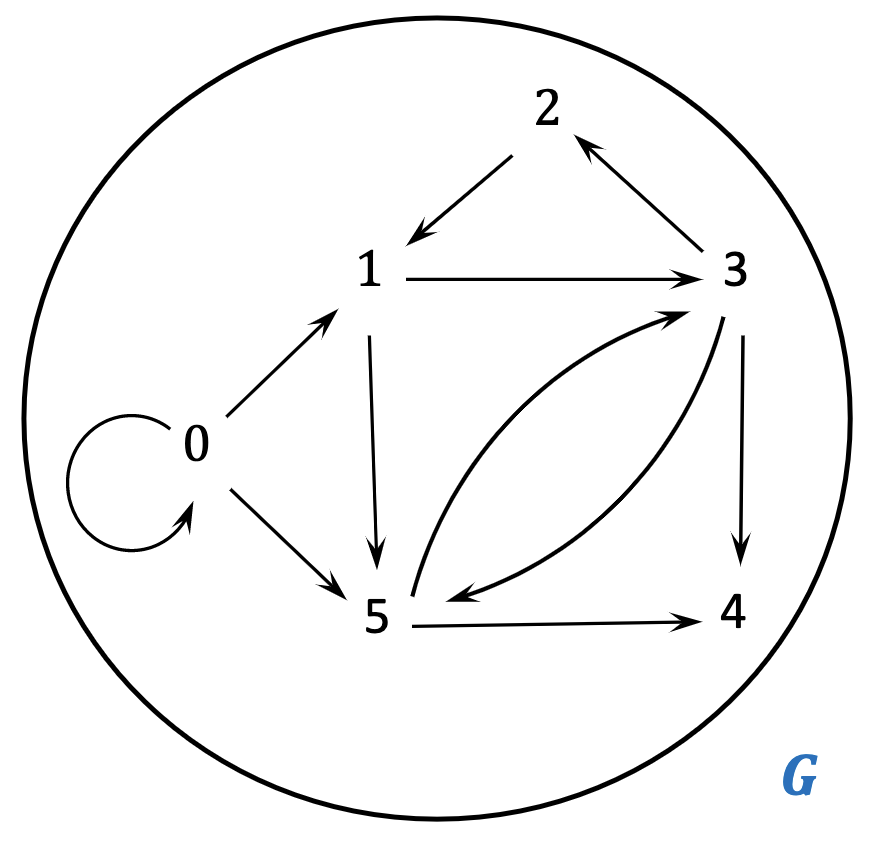
\includegraphics[width=3.3cm]{images/esempio-grafo.png}
        \caption{}
    \end{subfigure}
    \hfill
    \begin{subfigure}{.3\textwidth}
        \centering
        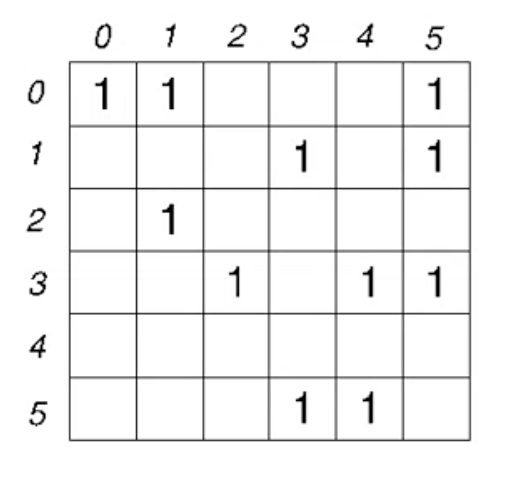
\includegraphics[width=3.3cm]{images/matrice-adiacenza.png}
        \caption{}
    \end{subfigure}
    \hfill
    \begin{subfigure}{.3\textwidth}
        \centering
        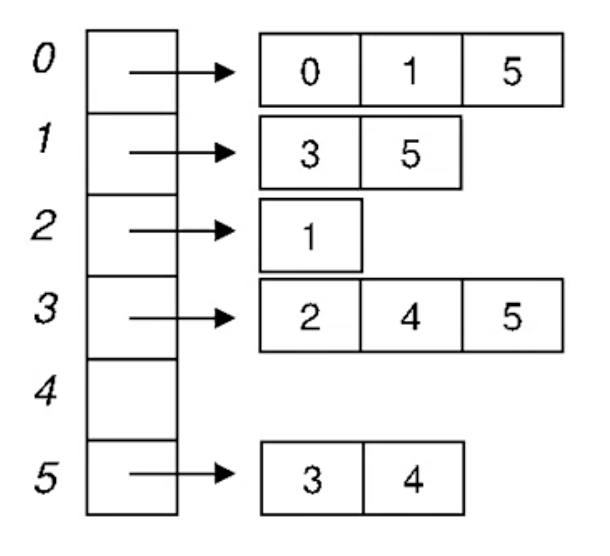
\includegraphics[width=3.3cm]{images/liste-adiacenza.png}
        \caption{}
    \end{subfigure}
    \vspace{-5pt}
    \caption{In (a) il grafo, in (b) la matrice di adiacenza ed in (c) la lista di adiacenza}
\end{figure}
\subsubsection{Matrici di adiacenza}
Una delle tecniche di rappresentazione di un grafo è tramite una matrice di adiacenza.
\begin{definition}[Matrice di adiacenza]
    La matrice di adiacenza di $G$ è una matrice quadrata $A$ con $n$ righe e $n$ colonne, numerate da $0$ a $n-1$, dove l'elemento di $A_ij$ (in riga $i$ e colonna $j$) assume un valore in $0$ se $(i,j) \notin E$ e $1$ se $(i,j) \in E$.
\end{definition}
Questo tipo di rappresentazione è molto utile per sfruttare tecniche di algebra lineare, ma non conviene in termine di spazio occupato se ci sono pochi archi da rappresentare.\\
Alcune proprietà dei grafi viste tramite le matrici di adiacenza:
\begin{itemize}
    \item Dato $x \in V$, $N^+(x)$ si ottiene guardando tutti gli $1$ nella riga $x$.
    \item Dato $x \in V$, $N^-(x)$ si ottiene guardando tutti gli $1$ nella colonna $x$.
    \item Per ottenere $|E|$ si sommano tutti gli $1$ nella matrice.
    \item $d^+_x$ si ottiene sommando gli $1$ di una riga.
    \item $d^-_x$ si ottiene sommando gli $1$ di una colonna.
\end{itemize}

\subsubsection{Liste di adiacenza}
Un metodo alternativo alle matrici di adiacenza sono le liste di adiacenza.
\begin{definition}[Liste di adiacenza]
    La rappresentazione con liste di adiacenza di un grafo orientato $G = (V,E)$ è costituita da un array di $A$ di $n = |V|$ insiemi in cui l'elemento i-esimo è il vicinato in uscita del nodo $i \in V$, cioè $A[i] = N^+(i)$.
\end{definition}
Questo tipo di rappresentazione occupa meno memoria delle matrici di adiacenza se $|E|$ è molto minore di $|V|^2$. Questo perché se prendiamo per esempio una $|E| = 10^{11}$ ed una $|V| = 10^9$ la rappresentazioni di una matrice occuperà $|V|^2$ spazi che sono uguali a $10^{18}$ mentre le liste occuperanno spazi uguali a $|V| + |E|$ che in questo caso sarebbero $10^9 + 10^{11}$ che è minore di della rappresentazione della matrice.\\
Alcune proprietà dei grafi viste tramite le matrici di adiacenza:
\begin{itemize}
    \item Dato $x \in V$, $N^+(x)$ si ottiene leggendo semplicemente la lista di adiacenza ad $x$.
    \item Dato $x \in V$, $N^-(x)$ si ottiene leggendo tutte le di di adiacenza e cercando occorrenze di $x$.
\end{itemize}

\subsection{Grafi orientati etichettati e pesati}
\begin{definition}[Grafo etichettato, grafo pesato]
    Un grafo orientato, etichettato o pesato è una tripla $G = (V,E,L)$ dove $L$ è una funzione $L: (V \cup E) \to D$ che associa ad ogni nodo e arco una etichetta presa da un certo dominio $D$ di valori. Nel caso che $D$ sia un valore numeri il grado si chiama anche pesato.
\end{definition}
La rappresentazioni di etichette su grafi orientati è simile a quella per grafi normali, quindi si possono usare le tecniche di matrici di adiacenza e di liste di adiacenza andando però nel primo caso ad aggiungere l'etichetta al posto del numero 1, mentre nelle liste di adiacenza gli elementi dell'array conterranno una coppia di valori: il nodo a cui è collegato e il valore dell'etichetta.
\begin{figure}[h!]
    \centering
    \begin{subfigure}{.3\textwidth}
        \centering
        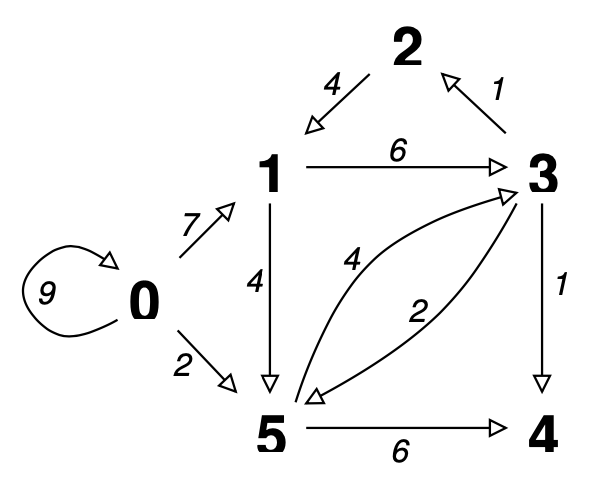
\includegraphics[width=3.5cm]{images/esempio-grafo-pesato.png}
        \caption{}
    \end{subfigure}
    \hfill
    \begin{subfigure}{.3\textwidth}
        \centering
        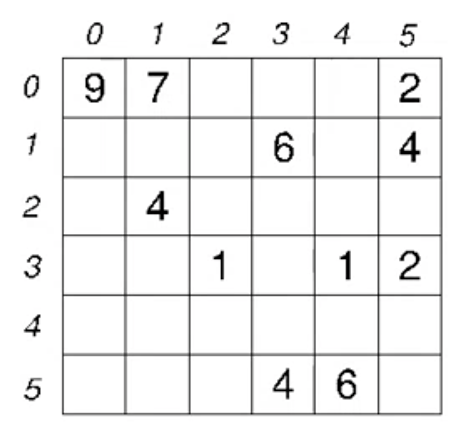
\includegraphics[width=3.5cm]{images/matrice-adiacenza-pesata.png}
        \caption{}
    \end{subfigure}
    \hfill
    \begin{subfigure}{.3\textwidth}
        \centering
        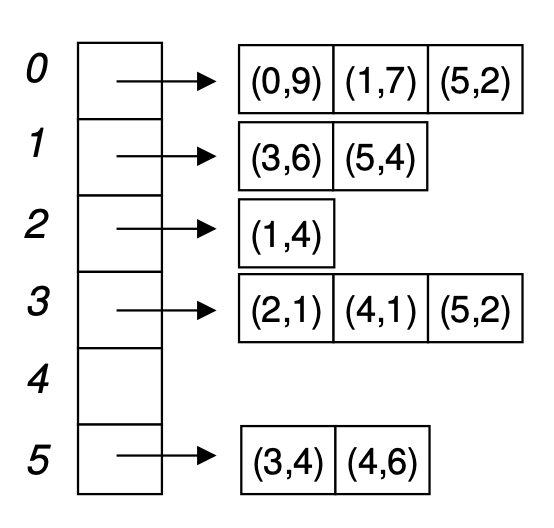
\includegraphics[width=3.5cm]{images/lista-adiacenza-pesata.png}
        \caption{}
    \end{subfigure}
    \vspace{-5pt}
    \caption{In (a) il grafo pesato, in (b) la matrice pesata ed in (c) la lista pesata}
\end{figure}

\newpage
\subsection{Cammini}
\begin{definition}[Cammino]
    Un \textbf{cammino} è una sequenza di nodi collegati da archi (nella stessa direzione).
\end{definition}

\subsubsection{Walk, trail e path}
Esistono 3 tipi di cammini: il \textbf{walk}, il \textbf{trail} ed il \textbf{path}
\begin{definition}[Walk]
    Dato un grafo orientato $G = (V,E)$ un \textbf{walk} è una sequenza di nodi.
    \begin{center}
        $P = v_0, v_1, \ldots, v_k$ tale che $(v_i,v_{i+1}) \in E$ per ogni $i \in K$
    \end{center}
\end{definition}
\hspace{-15pt}Vediamo che la \textbf{lunghezza} di $P$ è uguale a $k$ mentre gli estremi di un walk $P$ sono $v_0$ e $v_k$, e si dice che $P$ inizia con $v_0$ e termina con $v_k$.
\begin{note}
Un walk di lunghezza $0$ è un semplice nodo.
\end{note}

\begin{definition}[Trail e path]
    Un walk $P$ è detto \textbf{trail} se attraversa ogni arco in $E$ al più una volta. Un trail è detto \textbf{path} se attraversa ogni nodo in $V$ al più una volta.
\end{definition}

\begin{example}
    Prendendo come esempio l'immagine \ref{fig:esempio-grafo} vediamo che:
    \begin{itemize}
        \item La sequenza $\{0, 0, 1, 3, 2, 1, 3, 2\}$ è un walk ma non è un trail.
        \item Mentre la sequenza $\{0, 0, 1, 3, 4, 3, 4\}$ è un trail ma non è un path.
        \item Infine la sequenza $\{0, 1, 3, 4\}$ è un path.
    \end{itemize}
\end{example}

\subsubsection{Enunciati sui cammini}
\begin{proposition}\label{proposizione-walk-1}
Sia $G = (V,E)$ un grafo orientato e siano $x,y \in V$ due nodi. Allora vale che:
\begin{center}
    \footnote{Ricorda che $E^n$ è una composizione di$ $E per $n$ volte, quindi con $n=3$ è $E;E;E$}Esiste un walk di lunghezza $n\in \mathbb{N}$ da $x$ a $y$ $\Longleftrightarrow (x,y) \in E^n$
\end{center}
\end{proposition}
\begin{demostration}
Dimostrammo la proposizione \ref{proposizione-walk-1} per induzione.
\begin{enumerate}
    \item \underline{Caso base:} con $n=0$ può esistere un solo walk di lunghezza 0 e sarebbe un walk $(x,x)$ con il nodo $x \in V$. Questo caso si dimostra facilmente visto che $E^0 = Id_E$ e per definizione di identità $(x,x) \in Id_E$.
    \item \underline{Passo induttivo:} Per ipotesi induttiva assumiamo che il caso per un walk di lunghezza $n$ sia vero, dimostriamo ora che vale anche quello di lunghezza $n+1$. \\ \\
    Noi sappiamo che esista un walk di lunghezza $n + 1$ fra $x$ e $y$:
    \begin{enumerate}
        \item $\Longleftrightarrow \: \exists$ un walk $x, v_1, v_2, ..., v_n, y$ che a sua volta esiste.
        \item $\Longleftrightarrow (x, v_1) \in E$ ed esiste un walk $v_1, v_2, ..., v_n, y$, che esiste.
        \item $\Longleftrightarrow (x, v_1) \in E$ e $(v_1,y) \in E^n$.
        \item $\Longleftrightarrow (x,y) \in E^{n+1}$
    \end{enumerate}
    Nel (c) il primo passaggio del walk deve esistere già in $E$ ($E$ senza ulteriori composizioni$E^n$), il resto del walk invece è $(v_1,y) \in E^n$ e non in $n+1$ perché avendo "tolto" e messo a se il primo passo ($(x, v_1) \in E$) ci rimane un cammino di lunghezza $n$. Se quindi facciamo la composizione fra $E$ ed $E^n$ ($E;E^n$) torna che è uguale a dire $E^{n+1}$, quindi arriviamo al punto (d) che dimostra il passo induttivo. $\blacksquare$
\end{enumerate}
\end{demostration}

\newpage
\begin{lemma}\label{lemma-1}
    Sia $G=(V,E)$ un grafo orientato e siano $x,y \in V$ due nodi. Allora vale che:
    \begin{enumerate}
        \item Se esiste un walk da x a y $\Longrightarrow$ esiste un trail da x a y.
        \item Se il walk ha lunghezza $>0$, allora anche il trail ha lunghezza $>0$.
    \end{enumerate}
\end{lemma}
\begin{demostration}
Questo lemma può essere dimostrato intuitivamente in entrabi i suoi punti. \\ \\
\underline{Caso 1:} Innanzitutto partiamo da un walk P = 1,2,3,4,1,2,6,5 dove c'è almeno una ripetizione dello stesso arco (in questo caso si passa 2 volte fra 1,2) che quindi non lo rende un trail.\\
Possiamo però rendere questo walk un trail rimuovendo tutti i collegamenti da una all'altra coppia ripetuta (in questo caso si rimuove "3,4,1,2") visto che se 2 è connesso a 6 possiamo connetterlo direttamente senza passare per 3,4,1,2. Eseguendo questa operazione per tutte le ripetizioni otteniamo un trail. \\\\
\underline{Caso 2:} Se esiste un walk di lunghezza maggiore di 0 fra $x$ e $y$, come visto sopra, esisterà anche un trail fra $x$ e $y$, ma è immediato dire che se esiste un trail fra questi due nodi deve esistere almeno un arco che li collega e che quindi dimostra che la lunghezza è $>0$.
$\blacksquare$
\end{demostration}
\begin{figure}[h!]
    \centering
    \begin{subfigure}{.3\textwidth}
        \centering
        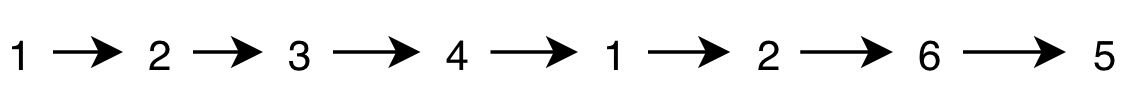
\includegraphics[width=5cm]{images/lemma-walk-trail-3.png}
        \caption{}
    \end{subfigure}
    \hfill
    \begin{subfigure}{.3\textwidth}
        \centering
        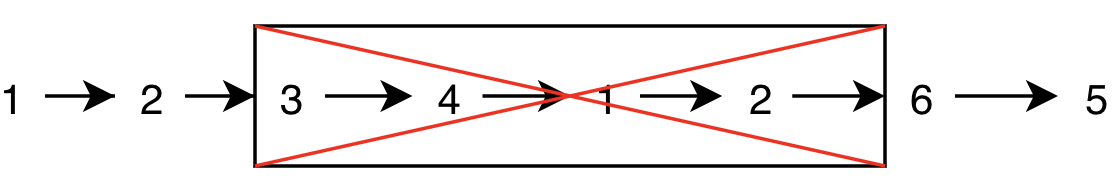
\includegraphics[width=5cm]{images/lemma-walk-trail-2.png}
        \caption{}
    \end{subfigure}
    \hfill
    \begin{subfigure}{.3\textwidth}
        \centering
        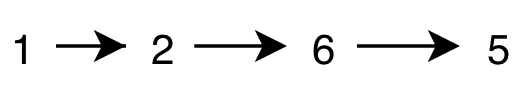
\includegraphics[width=3.5cm]{images/lemma-walk-trail-1.png}
        \caption{}
    \end{subfigure}
    \vspace{-5pt}
    \caption{Steps di trasformazione di un walk in un trail}
\end{figure}

\begin{lemma}\label{lemma-2}
Sia $G=(V,E)$ un grafo orientato e siano $x,y \in V$ due nodi. Allora vale che:
\begin{center}
    Se esiste un trail da x a y, allora esiste un path da x a y.
\end{center}
\end{lemma}
\begin{demostration}
Pure questo lemma si dimostra in maniera abbastanza intuitiva. Se prendiamo infatti un trail P = 4,5,6,7,6,9 che avendo una ripetizione di un nodo (il 6) non è un path, possiamo però farlo diventare andando a costruire un path rimuovendo il nodo ripetuto insieme a tutti i nodi intermedi (fra i due nodi doppi) e connettere il collegamento del nodo ripetuto al nodo mantenuto, riportato a questo esempio rimuoviamo 7,6 e connettiamo 9 a 4,5,6, questo fa uscire un path 4,5,6,9. Nel caso che con questa operazioni non sia ancora uscito un path basta ri-eseguirla per tutti i nodi ripetuti che rimangono. $\blacksquare$
\end{demostration}
\begin{figure}[h!]
    \centering
    \begin{subfigure}{.3\textwidth}
        \centering
        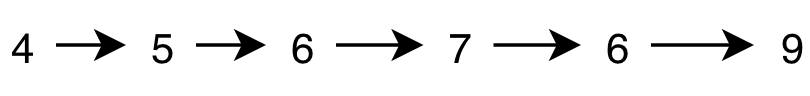
\includegraphics[width=5cm]{images/trail-path-1.png}
        \caption{}
    \end{subfigure}
    \hfill
    \begin{subfigure}{.3\textwidth}
        \centering
        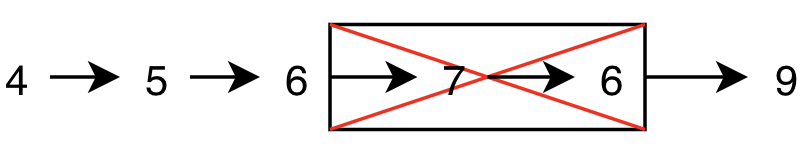
\includegraphics[width=5cm]{images/trail-path-2.png}
        \caption{}
    \end{subfigure}
    \hfill
    \begin{subfigure}{.3\textwidth}
        \centering
        \includegraphics[width=3.5cm]{images/trail-path-3.png}
        \caption{}
    \end{subfigure}
    \vspace{-5pt}
    \caption{Steps di trasformazione di un trail in un path}
\end{figure}

\subsubsection{Walk chiusi, circuiti, cicli}
Quando in un walk si parte e si termina sullo stesso nodo possiamo andare a definire tale cammino in uno di questi 3 modi.
\begin{definition}[Walk chiuso, circuito e ciclo]\label{walk-chiusi-circuiti-cicli}
    Dato un walk P esso si definisce \textbf{walk chiuso} se gli estremi sono lo stesso nodo. Un walk chiuso che è un trail si definisce \textbf{circuito}, mentre un circuito che è un path viene chiamato \textbf{ciclo} (Senza considerare gli estremi).
\end{definition}
\begin{definition}[Grafo ciclico]
    Un grafo G si dice \textbf{ciclico} se esiste almeno un ciclo in G, in caso contrario di dice aciclico
\end{definition}

\newpage
\begin{proposition}\label{proposizione-walk-2}
    Sia G = (V,E) un grafo orientato e x un nodi in V. Le seguenti affermazioni sono equivalenti:
    \begin{enumerate}
        \item Esiste un walk chiuso da x a x.
        \item Esiste un circuito da x a x.
        \item Esiste un ciclo da x a x.
        \item $(x,x) \in E^*$
    \end{enumerate}
\end{proposition}
\begin{demostration}
Anche questa proposizione si dimostrazione intuitivamente applicando gli enunciati visti prima. Innanzitutto partiamo a dimostrare che se (1) allora (2). Questa affermazione è vera per la proposizione \ref{lemma-1}. Dimostriamo ora che se (2) allora (3). Questo si dimostra rapidamente come prima applicando una proposizione vista in precedenza, in questo caso la \ref{lemma-2}. In fine per la proposizione \ref{proposizione-walk-1} (1) se e solo se (4). E così dimostrato che queste 4 affermazioni si equivalgono. $\blacksquare$
\end{demostration}


\subsection{Connettività}
\begin{definition}[Fortemente connesso]\label{grafo-fortemente-connesso}
    Dato un grafo orientato $G = (V,E)$ si dice che questo grafo è \textbf{fortemente connesso} se per ogni coppia di nodi $x,y \in V$ esiste un walk da $x$ a $y$.
\end{definition}
\begin{definition}[Componente fortemente connesso]\label{componente-fortemente-connesso}
    Una componente fortemente connessa (SCC) di $G$ è un sottoinsieme non vuoto di nodi $U \subseteq V$ tale che:
    \begin{enumerate}
        \item Per ogni coppia di nodi $x,y \in U$ esiste un walk da $x$ a $y$.
        \item Se esiste un $U' \subseteq V$ che soddisfa la $1$ e $U \subseteq U'$, allora $U = U'$ \footnote{$U$ si definisce sottoinsieme massimale}.
    \end{enumerate}
\end{definition}
\begin{example}
    Prendiamo per esempio l'immagine \ref{fig:esempio-SCC}:
\end{example}
\begin{wrapfigure}[9]{l}{6cm}
    \vspace{-10pt}
    \centering
    \includegraphics[width=3.7cm]{images/esempio-SCC.png}
    \caption{Grafo con i suoi SCC}
    \label{fig:esempio-SCC}
\end{wrapfigure}
In questa immagine vediamo che se prendiamo un sottoinsieme U = $\{5,4\}$ esso non è un SCC perchè non è validato il punto (2) visto che esiste un sottoinsieme $U' = \{1,3,5\}$ che lo contiene. \\Anche $U'$ non è un SCC mentre se prendiamo come $U = \{1,2,3,5\}$ questo è un SCC visto che c'è un walk per ogni elemento ed è il sottoinsieme massimale.\\
In questo esempio risulta che i SCC sono: 
\begin{center}
    $\{1,2,3,5\}$, $\{4\}$, $\{0\}$
\end{center}

\subsubsection{Componenti connesse e partizioni}
\begin{proposition}
    Dato un grafo $G=(V,E)$, l'insieme delle componenti fortemente connessi di $G$ è una partizione di $V$.
\end{proposition}
\begin{demostration}
Andiamo ora a dimostrare questa proposizione. Innanzitutto ricordiamo che $P = \{A_i\}_{i \in I}$ è una partizione dell'insieme $A$ se rispetta queste 3 condizioni:
\begin{enumerate}
    \item $\forall i$ $A_i \neq \O$
    \item $\bigcup^m_{i=1}A_j = A$
    \item $\forall i, j A_i \cap A_j = \O$ con $i \neq j$
\end{enumerate}
Quello che noi dobbiamo dimostrare è che l'insieme SCC = $\{C_1, C_2, \ldots, C_k\}$ è un partizione di $G$.
\begin{enumerate}
    \item La prima si dimostra immediatamente, perché un componente fortemente connesso non può essere vuoto per la sua definizione \ref{componente-fortemente-connesso}.
    \item Il secondo punto si dimostra prendendo una $x \in V$ e un insieme $U = \{x\}$, il quale rispetta la condizione (1) della definizione \ref{componente-fortemente-connesso}. Ora questo insieme può o essere una partizione, oppure esser contenuto in una componete fortemente connesso; capiamo dunque che se ripetiamo questa operazione per ogni elemento dell'insieme $V$ avremo una serie di SCC che alla peggio saranno tutti insiemi di un elemento o al meglio sarà tutto $V$, in ogni caso comunque ogni elemento apparterrà alla fine ad un SCC che se andiamo ad unire tutti insieme avremo $V$.
    \item Andiamo a dimostra il terzo punto per assurdo.\\ 
    Supponiamo che $\exists C_i, C_j$ partizioni distinte $\mid C_i \cap C_j \neq \O$. Se questa condizione è vera allora $\exists x \in C_i \cap C_j$ e $\exists y \in C_i \setminus C_j$ e anche $\exists z \in C_j \setminus C_i$ per definizione di intersezione.\\\\
    Se però la condizione che abbiamo posto per assurdo è vera allora $\forall \: y \in C_i$ e $\forall \: z \in C_j \Longrightarrow C_i \cup C_j$ soddisfa la proprietà (1) della definizione \ref{componente-fortemente-connesso}, e quindi che:\\
    $\exists$ walk $y \ldots x$, $\exists$ walk $x \ldots z \Longrightarrow \exists$ walk $y \ldots z$\\
    $\exists$ walk $z \ldots x$, $\exists$ walk $x \ldots y \Longrightarrow \exists$ walk $z \ldots y$ \\
    e questo dovrebbe avvenire perché se $C_i \cap C_j \neq \O$ vuol dire che c'è un elemento in comune in entrambi gli insieme che per la proprietà (1) dovrà avere un walk con gli altri elementi sia di $C_i$ che di $C_j$.
    Ma se ciò accadesse gli insiemi stessi $C_i$ e $C_j$ non sarebbero più partizioni perché sarebbe violata la proprietà (2) della definizione esistendo un insieme $C_i \cup C_j$ che li contiene. $\blacksquare$
\end{enumerate}
\end{demostration}

\subsubsection{Proprietà connettività}
\begin{proposition}\label{proposizione-connettività-1}
    Per tutti i grafi orientati $G=(V,E)$ e tutti gli $x,y \in V$ vale che:
    \begin{enumerate}
        \item $G$ è fortemente connesso $\Longleftrightarrow V \times V \subseteq E^*$.
        \item $(x,y) \in E^* \cap (E^*)^{op} \Longleftrightarrow$ $x$ ed $y$ appartengono alla stessa componente fortemente connessa.
    \end{enumerate}
\end{proposition}
\begin{demostration} \label{dimostrazione-prop-1}
Questo due proprietà sono vere perché:
\begin{enumerate}
    \item Nella prima dire di avere un grafo fortemente connesso vuol dire avere un grafo che per ogni $x, y \in V \times V$ nodi esiste un walk fra essi, ma ciò e vero se e solo se (per la proposizione \ref{proposizione-walk-1}) per ogni $x, y \in V \times V$ val che  $(x,y) \in E^*$\footnote{Ricorda che la stella di kleene applica la chiusura transitiva per rendere appunto transitivo l'insieme, quindi applica una sequenza di composizioni, che è lo stesso di $E^n$}, ma se ogni $(x,y)$ appartengono sia a $V \times V$ che a $E^*$ possiamo scrivere che $V \times V \subseteq E^*$ (non il viceversa perché la stella di kleene include anche la proprietà riflessiva).
    \item Per dimostrare la seconda consideriamo che se esiste un walk fra $x$ e $y$ e viceversa vuol dire che $x$ e $y$ fanno parte della stessa componente fortemente connessa e quindi $(x,y) \in E^*$ per la dimostrazione vista sopra, e $(x,y) \in (E^*)^{op}$, e questo perché: se lo vediamo come $(x,y) \in (E^{op})^*$ (possibile per le proprietà della stella di kleene) quello che facciamo è andare ad invertire tutti gli archi in E e poi aggiungere la chiusura di kleene che, aggiungendo la proprietà transitiva all'insieme, fa si che esista un walk fra (x,y); quindi in conclusione visto che ($x,y$) apparitene ad entrambi gli insiemi apparterrà anche alla loro composizione $(x,y) \in E^* \cap (E^*)^{op}$. $\blacksquare$
\end{enumerate}
\end{demostration}

\subsection{Grafo orientato aciclico (DAGs)}
\begin{definition}[DAG, Sorgenti, Pozzi]
    Un grafo orientato senza cicli si chiama \textbf{Directed Acyclic Graph (DAG)}. Al suo interno possono esistere uno o più nodi di grado di ingresso $0$ detti \textbf{sorgenti} e uno o più nodi di grado di uscita $0$ detti \textbf{pozzi}
\end{definition}

\begin{proposition}
    Se $G = (V,E)$ è un DAG, allora $E^*$ è un ordinamento parziale.
\end{proposition}
\begin{demostration}
Per dimostrare che un grafo è un DAG, allora la stella di Kleene sugli archi ($E^*$) è un ordinamento parziale. Bisogna quindi dimostrare le 3 proprietà che rendono una relazione su un insieme un ordinamento parziale, e cioè la \textbf{transitività}, la \textbf{anti-simmetria} e la \textbf{riflessività}.
\begin{itemize}
    \item \underline{Dimostrazione \textbf{transitiva} e \textbf{riflessiva}}: Queste due proprietà si dimostrano velocemente visto che la stella di Kleene aggiunge sia la proprietà transitiva che riflessiva all'insieme.
    \item \underline{Dimostrazione \textbf{anti-simmetrica}}: Per dimostrare questa proprietà basta, per il punto (4) del teorema di caratterizzazione \ref{teorema-caratterizzazione}, andare a dimostrare che $E^* \cap (E^*)^{op} \subseteq Id_V$.\\
    Ora noi sappiamo che se $(x,y) \in E^* \cap (E^*)^{op}$ esiste un walk fra $x$ e $y$ e viceversa per la proposizione \ref{proposizione-walk-1} (questo perché come anche descritto nella dimostrazione \ref{dimostrazione-prop-1} la stella di Kleene aggiunge una concatenazione di composizioni). Se poniamo per assurdo che $x \neq y$ quello che risulterebbe sarebbe un walk chiuso che attraversa entrambi, perché se esiste un walk ($x,y$) ed uno ($y, x$) esso crea un ciclo, ma questo non può essere possibili perché abbiamo supposto per ipotesi che $G$ sia un DAG. Quindi risulta che $x = y$. $\blacksquare$
\end{itemize}
\end{demostration}

\subsubsection{Ordinamento topologico}
\begin{definition}
    Dato un DAG $G = (V,E)$ un ordinamento topologico di $G$ è una biiezione $\eta: V \to n$ con $n = \{0,1,2,\ldots, n-1\}$ \footnote{Si ricorda che per la definizione vista nel capitolo 1 ogni numero naturale $n$ denota un insieme}tale che:
    \begin{equation}
        \textbf{per ogni arco } (u,v) \in E \textbf{ vale } \eta(u) < \eta(v)
    \end{equation}
\end{definition}
\hspace{-15pt}In altre parole, se disponiamo i vertici lungo una linea orizzontale in base alla loro numerazione $\eta$, in ordine crescente, otteniamo che gli archi risultano tutti orientati da sinistra verso destra
\begin{proposition}
    Ogni DAG ha almeno un ordinamento topologico, e ne possono esistere di più.
\end{proposition}

\subsection{Grafo non orientato}
\begin{definition}[Grafo non orientato]
    Un grado non orientato $G = (V,E)$ ha un insieme finito di nodi $V$ e un insieme di archi $E = P_2(V)$ dove $P_2(V) = \{X \subseteq V \mid |X| = 2\}$
\end{definition}
\begin{wrapfigure}[8]{l}{6cm}
    \vspace{-15pt}
    \centering
    \includegraphics[width=3.7cm]{images/esempio-grafo-non-orientato.png}
    \vspace{-5pt}
    \caption{Grafo G non oriento}
    \label{fig:esempio-grafo-non-orientato}
\end{wrapfigure}
La caratteristica principale dei grafi non orientati è che gli archi non hanno una direzione, quindi sono sottoinsiemi di nodi di cardinalità $2$. Scriviamo un arco fra $x$ ed $y$ come $xy \in E$, ovvero $\{x,y\} \in E$. Un grafo orientato inoltre non può avere cappi.\\ \\
Quello in figura \ref{fig:esempio-grafo-non-orientato} è un esempio di grafo non orientato. \\\\\\\\
\textbf{Notazione.} Alcune definizioni e notazioni sui grafi non orientati. Dato un grafo $G = (V,E)$ non orientato si dice che:
\begin{itemize}
    \item Il \textbf{vicinato} di un nodo $x \in V$: \hspace{.7cm} $N(x) = \{y \in V \mid xy \in E\}$
    \item Il \textbf{grado} di un nodo $x \in V$: \hspace{.7cm} $d_x = \lvert N(x)\rvert$.
\end{itemize}
\begin{definition}[Universale, Isolato]
    Un nodo $x$ si dice Univalente se è vicino di tutti i nodi quindi $N(x) \cup \{x\} = V$, mentre un nodo si dice isolato se non ha vicinato, quindi $N(x) = \O$
\end{definition}

\begin{definition}[Grafo orientato associato]
    Dato un grafo non orientato $G = (V,E)$, quindi un grafo con $E \subseteq P_2(V)$, il \textbf{grafo orientato associato} a $G$ è il grafo orientato $\widetilde{G} = (V, \widetilde{E})$, dove la relazione $\widetilde{E}$ è definita come:
    \begin{center}
        $\widetilde{E} = \{(x,y) \in V \times V \mid \{x,y\} \in E\}: V \leftrightarrow V$
    \end{center}
\end{definition}

\begin{figure}[h!]
    \centering
    \begin{subfigure}{.3\textwidth}
        \centering
        \includegraphics[width=3.5cm]{images/grafo-non-orientato.png}
        \vspace{-5pt}
        \caption{}
    \end{subfigure}
    \hspace{1cm}
    \begin{subfigure}{.3\textwidth}
        \centering
        \includegraphics[width=3.5cm]{images/grafo-orientato-associato.png}
        \vspace{-5pt}
        \caption{}
    \end{subfigure}
    \caption{In (a) il grafo non orientato ed in (b) il rispettivo grafo non associato}
\end{figure}

\subsubsection{Hand-shaking lemma}
	L'hand-shaking lemma varia per i grafi non orientatati rispetto a come era definito per quelli orientati.
\begin{lemma}[Hand-shaking lemma]
    Per ogni grafo non orientato $G = (V,E)$, vale che:
    \begin{center}
        $\sum\limits_{x \in V}d_x = 2\lvert E\rvert$
    \end{center}
    Esso dice infatti che la somma dei gradi di tutti i nodi è uguale a $2$ volte il numero di archi del grafo. 
\end{lemma}
Il lemma è valido perché: osservando che con l'aggiunta di un arco in un grafo si va a incrementare di $1$ il grado di $2$ nodi differenti, visto che un arco dovrà per forza connettere due nodi che non possono essere lo stesso (non esistendo il cappio), aumenterà di $2$ volta la somma di tutti i gradi, mentre aumenterà solo di $1$ il numero di archi, avendo aggiunto un solo arco, basta dunque andare a moltiplicare per $2$ il numero di archi per ottenere la somma dei gradi.

\subsubsection{Rappresentazione grafi non orientati}
Le rappresentazioni per i grafi non orientati sono similari a quelle dei grafi orientati. Esiste infatti sia la rappresentazione tramite \textbf{matrice di adiacenza} che tramite \textbf{lista di adiacenza}; le uniche differenze sono che, non esistendo un verso per gli archi, verranno riscritti $2$ volte i collegamenti, uno per ogni direzione, questo sia nelle matrici che nelle liste.
\begin{figure}[h!]
    \centering
    \begin{subfigure}{.3\textwidth}
        \centering
        \includegraphics[width=3.3cm]{images/esempio-grafo-non-orientato.png}
        \caption{}
    \end{subfigure}
    \hfill
    \begin{subfigure}{.3\textwidth}
        \centering
        \includegraphics[width=3.3cm]{images/matrice-grafo-non-orientato.png}
        \caption{}
    \end{subfigure}
    \hfill
    \begin{subfigure}{.3\textwidth}
        \centering
        \includegraphics[width=3.3cm]{images/lista-grafo-non-orientato.png}
        \caption{}
    \end{subfigure}
    \vspace{-5pt}
    \caption{In (a) il grafo non orientato, in (b) la matrice ed in (c) la lista di adiacenza}
\end{figure}

\subsubsection{Cammini nei grafi non orientati}
\begin{definition}[Walk]
    In un grafo non orientato $G = (V,E)$, un walk è una sequenza di nodi
    \begin{center}
        $P = v_0, \ldots, v_k$ tale che $\{v_i, v_i+1\} \in E$ per ogni $i \in K$
    \end{center}
    La lunghezza del walk $P$ è uguale a $k$.
\end{definition}

\begin{definition}[Trail, path]
    Si definisce trail un walk che non attraversa due volte lo stesso arco. Un path è un walk (o trail) che non attraversa due volte lo stesso nodo.
\end{definition}

Le proposizioni \ref{proposizione-walk-1}, \ref{proposizione-walk-2} e i lemmi \ref{lemma-1}, \ref{lemma-2}  sono validi in ugual modo per i grafi non orientati, bisogna solo tenere in considerazione il fatto che in questo tipo di grafi gli archi non hanno verso (in pratica bisogna sostituire la $E$ con $\widetilde{E}$), le dimostrazioni sono similari.

\subsubsection{Cicli e connettività nei grafi non orientati}
Per i grafi non orientati le definizioni di \textbf{walk chiuso}, \textbf{circuiti} e \textbf{cicli} sono uguali a quelli visti nei grafi orientati (Definizione \ref{walk-chiusi-circuiti-cicli}).
\begin{note}
Un walk chiuso (da $x$ a $x$) non implica un circuito (da $x$ a $x$), ma un circuito implica un ciclo
\end{note}
Ugualmente le definizioni di grafo \textbf{fortemente connesso} e  di \textbf{componente fortemente connesso} sono analoghe a quelle viste per i grafi orientati (Definizioni \ref{grafo-fortemente-connesso}, \ref{componente-fortemente-connesso}).\\
Anche qui, la proposizione \ref{proposizione-connettività-1} vale  per i grafi non orientati (bisogna sostituire la $E$ con $\widetilde{E}$).


\subsection{Cammini Euleriani}
\begin{definition}[Circuito e trail euleriano]
    Dato un grafo non orientato connesso $G = (V,E)$, un \textbf{circuito euleriano} è un circuito che passa esattamente una volta per tutti gli archi del grafo. Analogamente un \textbf{trail euleriano}. (conosciuto anche come percorso euleriano)
\end{definition}
Questa definizione parte del problema dei sette ponti di Konigsberg.
\begin{theorem}[Il teorema di Eulero]
Dato un grafo $G = (V,E)$ non orientato e connesso:
\begin{enumerate}
    \item Esiste un circuito euleriano $\Longleftrightarrow$ tutti i nodi hanno grado pari.
    \item Esiste un trail euleriano da $x$ a $y$, con $x \neq Y$ $\Longleftrightarrow$ $x$ a $y$ sono gli unici nodi di grado dispari.
\end{enumerate}
\end{theorem}

\begin{demostration}
Dimostrazione dei due punti del teorema di Eulero.\\\\
\underline{Punto (1)}: Per andare a dimostrare questo punto dobbiamo dimostrare i due sensi della freccia.
\begin{itemize}
    \item Se esiste un circuito euleriano $\Longrightarrow$ tutti i nodi hanno grado pari.\\
    Questo caso è facilmente dimostrabile perché: possiamo notare che ogni volta che in un circuito euleriano noi passiamo per un nodo ($x \to y \to z$) attraversiamo $2$ archi mai attraversati, questo vuol dire che il numero di archi incidenti\footnote{Ricorda che gli archi incidenti sono gli archi che escono/entrano in un nodo, in un grafo non orientato} in un nodo è il doppio delle volte in cui il circuito ci passa, inoltre non può verificarsi una casistica in cui un nodo ha solo un arco perché in quel modo non ci verificherebbe un circuito.\\ Essendo che il numero di archi incidenti ad un nodo è il doppio non potrà mai essere un numero dispari.
    \item Se tutti i nodi hanno grado pari $\Longrightarrow$ esiste un circuito euleriano.\\
    Innanzitutto prendiamo un nodo $r$ ed iniziamo a creare un percorso in G marcando ogni arco in cui passiamo in modo da non passarci una seconda volta, a questo punto solamente $r$ avrà un solo arco incidente marcato all'inizio, mentre ogni nodo in cui passiamo avrà due archi marcati (un per arrivarci ed uno per andare), continueremo finché non ritorneremo nel nodo $r$ creando un circuito, non potrà essere altrimenti perché se il nodo finale $u \neq r$ allora vorrebbe dire che ha un numero di archi incidenti dispari (avendo un arco per arrivarci e non uno per uscirci) e questo non è possibile per ipotesi.\\\\
    A questo punto chiamiamo il circuito trovato C, se C passa per tutti gli archi allora è euleriano ed abbiamo finito, in caso contrario dobbiamo utilizziamo l'ipotesi che G sia connesso per così dedurre che esista un nodo $r'$ in C che ha un arco incidente non marcato.\\\\ 
    Prendiamo ora $r'$ e ripetiamo l'operazione vista prima andando a ricreare un nuovo circuito $C'$, notiamo che $C'$ e $C$ sono disgiunti sugli archi (perché marchiamo man mano gli archi che passiamo), inoltre $C$ e $C'$ si incontreranno in $r'$. \\\\
    A questo punto avremo due circuiti $C$ e $C'$ che coincidono in un nodo $r'$ e con tutti archi disgiunti, se quindi andiamo ad unire questi due circuiti prendendo come nodo di partenza e di arrivo $r'$ avremo un circuito che o è euleriano o avrà un nodo $r''$ con un arco non segnato, vediamo dunque che possiamo nuovamente ripetere l'operazione precedentemente vista altre $n$ volte, andando volta in volta a combinare i circuiti trovati fino a che non si creerà un circuito euleriano. $\blacksquare$
\end{itemize}
\underline{Punto (2)}: Anche qui bisogna dimostrare i due sensi della freccia per dimostrare la sua veridicità.
\begin{itemize}
    \item Se esiste un trail euleriano da $x$ a $y$, con $x\neq y \Longrightarrow$ $x$ e $y$ sono gli unici nodi di grado dispari.\\
    Questo verso lo dimostriamo vedendo che ogni volta che attraverso un nodo $v$ utilizzo $2$ archi, uno per entrare ed uno per uscire, le uniche eccezioni sono per il nodo di partenza e per quello di arrivo che avranno grado uguale a $2k + 1$ dove $k$ è il numero di volte in cui si passa per quel nodo (esclusa la partenza o l'arrivo) ed il $+1$ indica appunto la partenza nel caso di $x$ e l'arrivo nel caso di $y$. Abbiamo così dimostrato il primo verso.
    \item Se $x$ e $y$ sono gli unici nodi di grado dispari $\Longrightarrow $ esiste un trail euleriano da $x$ a $y$.\\
    Prendiamo per dimostrare questo caso un grado G = (V,E) che sua un grado connesso con $x,y \in V$ di grado dispari e $\forall v \in V . v\notin \{x,y\}$ siano di grado pari (queste condizioni sono vere per l'ipotesi).\\
    Ora creiamo un nuovo grafo $G'$ uguale a G solo introducendo un nuovo nodo $z$ con due archi $\{z,x\}$ e $\{z,y\}$ (questo nuovo nodo rispetta le condizioni poste nell'ipotesi). \\
    $G'$ è connesso visto che il nodo $z$ è connesso ad almeno un nodo il quale, appartenendo anche al grafo G che era connesso per ipotesi, è collegabile a tutti gli altri nodi, dunque che $z$ lo sarà, e quindi $G'$ è connesso.\\
    Essendo che $G'$ + connesso tutti, tutti i odi hanno grado pari $\exists$ circuito euleriano per il punto (1) di questo teorema. Ma visto che esiste un circuito euleriano $z,x,\ldots,y,z$ esisterà allora un trail $x,..,y$ che sarà euleriano nel caso si consideri il grafo $G$ (quindi senza $z$ e i suoi archi). Così dimostriamo anche questa implicazione. $\blacksquare$
\end{itemize}
\end{demostration}

\subsection{Cicli e path Hamiltoniani}
\begin{definition}[Cicli e path Hamiltoniani]
    Dato un grafo connesso (orientato o non orientato), un \textbf{ciclo hamiltoniano} è un ciclo che passa esattamente una volta per tutti i nodi del grafo. Analogamente, path hamiltoniano.
\end{definition}
Questo tipo di cammino non prevede una caratterizzazione semplice come per i circuiti euleriani. Equivale inoltre a cercare una permutazione dei nodi che formano un path.

\subsubsection{Il problema del commesso viaggiatore}
Il problema del commesso viaggiatore consiste, dato un grafo pesato non orientato, di trovare un ciclo hamiltoniano di peso minimo, dove il peso è la somma dei pesi degli archi attraversati.
\begin{figure}[h!]
    \centering
    \begin{subfigure}{.3\textwidth}
        \centering
        \includegraphics[width=3.3cm]{images/es-problema-viaggiatore-1.png}
        \caption{}
    \end{subfigure}
    \hfill
    \begin{subfigure}{.3\textwidth}
        \centering
        \includegraphics[width=3.3cm]{images/es-problema-viaggiatore-2.png}
        \caption{}
    \end{subfigure}
    \hfill
    \begin{subfigure}{.3\textwidth}
        \centering
        \includegraphics[width=3.3cm]{images/es-problema-viaggiatore-3.png}
        \caption{}
    \end{subfigure}
    \caption{(a) il grafo pesato, (b) ciclo hamiltoniano in (c) un ciclo hamiltoniano di peso minimo}
\end{figure}

\subsection{Distanze}
\begin{definition}[Distanza]
    Una \textbf{distanza} (o metrica) su un insieme A è una funzione $d: A \times A \to \mathbb{R}$ che soddisfa le seguenti proprietà per ogni $x,y,z \in A$.
    \begin{enumerate}
        \item $d(x,y) \geq 0$.
        \item $d(x,y) = 0 \Longleftrightarrow x = y$.
        \item $d(x,y) = d(y,x)$ (simmetria).
        \item $d(x,y) \leq (x,z) + d(z,y)$ (disuguaglianza triangolare)
    \end{enumerate}
\end{definition}
Si può notare che tutte queste condizioni sono soddisfatte dalla distanza euclidea \footnote{Ricorda che la distanza euclidea è la distanza fra due punti in un piano cartesiano}, infatti (1) la distanza euclidea è sempre maggiore o uguale a 0, e se è 0 è perché abbiamo preso due punti uguali (2), inoltre (3) la distanza fra due elementi non cambia, indipendentemente da quale punto prendiamo per prima, ed in fine in un triangolo la somma delle lunghezze di due lati  maggiore o uguale a quella del terzo lato (4).

\begin{definition}[Distanza su un grafo non orientato]
    Sia $G = (V,E)$ un grafo non orientato connesso. Dati due nodi $x,y \in V$, la loro \textbf{distanza} $d(x,y)$ è la lunghezza del walk più breve tra $x$ e $y$ (il cammino minimo).
\end{definition}
Possiamo vedere che in quest'ultima definizione sono rispettate i quattro punti della definizione di distanza.
\begin{enumerate}
    \item La distanza fra $x$ e $y$ è sempre $\geq 0$ perché in caso contrario vorrebbe dire che non esiste, e ciò non è possibile per la definizione stessa (nella definizione diciamo che il grafo è connesso).
    \item Se la distanza fra due nodi è $0$ allora il nodo è lo stesso.
    \item Se esiste un cammino da $x$ a $y$ con una certa distanza, questo cammino può essere percorso anche da $y$ a $x$ e quindi mantiene la stessa distanza.
    \item Essendo la distanza la lunghezza del walk più breve la distanza fra $x$ e $y$ sarà per forza minore o uguale di quella fra $x$ e $z$ sommata con quella fra $z$ e $y$.
\end{enumerate}

\begin{definition}[Distanza su grafo induttivamente]
    Sia $G = (V,E)$ un grafo non orientato connesso. Dati due nodi $x,y \in V$, al loro distanza $d(x,y)$ può essere definita induttivamente:
    \begin{itemize}
        \item \underline{Caso base}: $d(x,y) = 0$, se $x = y$.
        \item \underline{Passo induttivo}: $d(x,y) = 1 + min\{d(z,y) \mid z\in N(x)\}$. Dove $N(x)$ è il vicinato di $x$
    \end{itemize}
\end{definition}

La definizione di distanza (come lunghezza del cammino minimo) si può applicare anche a grafi orientati fortemente connessi, ma in questo caso non vengono rispettate tutte le proprietà:
\begin{enumerate}
    \item $d(x,y) \geq 0$ è vera per la definizione di grafo fortemente connesso.
    \item $d(x,y) = 0$ se e solo se $x = y$ è vera perché l'unico cammino di lunghezza $0$ è quello fra un nodo e se stesso.
    \item $d(x,y) = d(y,x)$ invece non è rispetta perché essendoci un verso negli archi possono esistere percorsi più brevi differenti.
    \item Visto che il punto (3) non è verificato non è necessario verificare il (4).
\end{enumerate}
Nel caso di grafi fortemente orientati definiamo la funzione della distanza una quasi-metrica.

\begin{proposition}\label{proposizione-distanza-1}
    Sia $G = (V,E)$ un grafo orientato connesso e $x$ un nodo. Sia $y$ un nodo a distanza massima da $x$, allora $G\setminus \{y\}$ è connesso.
\end{proposition}

\begin{demostration}
    Dimostriamo la proposizione scritta sopra, essa dice che:
    \begin{center}
        $\forall v \in V, d(x,y) \geq d(x,v) \Longrightarrow \forall v \in V \setminus \{y\}$ $\exists$ path $P = x,\ldots,v$. che non include y.
    \end{center}
    I path $P = x,\ldots,v$ non devono includere y perché se lo includesse allora $\exists$ $P' = x\ldots,y$ più corto di $P$ e questo contraddice che $d(x,y) \geq d(x,v)$.\\
    Se dal nostro grafo rimuovo y segue per quanto detto prima che $\forall v \in V \setminus \{y\}$ esiste ancora un path $P = x,\ldots,v$.
    Allora vediamo che $\forall v,w$ $\exists$ walk $W = v,\ldots,x,\ldots,w \Longrightarrow G \setminus \{y\}$ è connesso. $\blacksquare$
\end{demostration}

\subsubsection{Diametro, altezza, profondità}
\begin{definition}[Diametro di grafo]
    Il diametro di un grafo $G$ (oriento o meno) è la massima distanza tra coppie di nodi:
    \[diam(g) = \max_{x,y \in V}d(x,y)\]
\end{definition}

\begin{definition}[Profondità, altezza di nodi, albero pieno]
    Dato un albero radicato, la \textbf{profondità} di un nodo $x$ è la distanza $d(x,t)$ dalla radice $r$, e \textbf{l'altezza} di $x$ è la massima distanza tra $x$ e le sue foglie discendenti. L'altezza dell'albero è l'altezza della radice. Inoltre definiamo un albero cardinale come \textbf{pieno} se è completo e le foglie sono tutte alla stessa distanza dalla radice.
\end{definition}



\newpage
\subsection{Alberi}

\begin{definition}[Albero, foglia]
    Un \textbf{albero} è un grafo non orientato connesso, aciclico e non vuoto (con almeno $1$ nodo).
    I nodi interni hanno quindi grado $>1$ mentre i nodi di grado $1$ sono detti \textbf{foglie}.
\end{definition}

\begin{definition}[Foresta]
    Una \textbf{foresta} è un grafo non orientato, aciclico e non vuoto dove ogni componente connessa è un albero assestante.
\end{definition}
\hspace{-15pt}Da queste definizioni possiamo dedurre alcune proprietà relative agli alberi.
\begin{wrapfigure}[8]{r}{7cm}
    \centering
    \includegraphics[width=5cm]{images/es-albero.png}
    \vspace{-5pt}
    \caption{Esempio di albero}
\end{wrapfigure}
\begin{itemize}
    \item Il numero di path possibili fra due nodi è sempre uno, perché se esistessero due path distinti la concatenazione di questi due path sarebbe un walk chiuso e quindi il grafo avrebbe cicli (ricorda la proposizioni \ref{proposizione-walk-2} che ci dice che dire walk chiuso o ciclo è analogo).
\end{itemize}

\begin{itemize}
    \item Se andiamo a toglie un arco in un albero si andrà a creare una foresta con 2 alberi.
    \item Se invece andiamo ad aggiungere un arco quello che uscirà non sarà più un albero perché si creerà un ciclo.
\end{itemize}


\begin{proposition}
    Dato un albero G = (V,E) con $n = |V|$ nodi, valgono le seguenti proprietà:
    \begin{enumerate}
        \item Se $n \geq 2$ (ovvero l'albero ha almeno due nodi), allora G ha almeno una foglia (ovvero un nodo di grado 1).
        \item G ha esattamente $n-1$ archi, cioè $|E| = n-1$.
        \item Per ogni coppia di nodi distinti $x,y \in V$, esiste un unico path da x a y.
        \item Per ogni arco $xy \in E$, la rimozione di $xy$ rende il grafo non connesso.
        \item Per ogni coppia di nodi distinti $x,y \in V$ tale che $xy \notin E$, l'aggiunta dell'arco xy crea un ciclo, cioè $G' = (V, E \cup {xy})$ è un ciclo.
    \end{enumerate}
\end{proposition}


\begin{demostration}
Andiamo ora a dimostrare ogni punto della proposizione sopra.
\begin{enumerate}
    \item Per dimostrare il primo punto prendiamo innanzitutto un albero T = (V,E) con almeno 2 nodi, per la proposizione \ref{proposizione-distanza-1} $\exists y \in V \: |\: T \setminus \{y\}$ è connesso $\Longrightarrow T \setminus \{y\}$ rimane connesso quindi rimane un albero.\\
    Ora, se re-introduciamo y possiamo vedere 2 casi:
    \begin{itemize}
        \item O $|N(y)| = 1$ (il vicinato di $y$ è 1), quindi $y$ è una foglia di T e la proprietà e verificata.
        \item Oppure $|N(y)| \geq 2$ (il vicinato di $y$ è maggiore o uguale a 2), in questo caso però $\exists$ path $P = w,...,z$ in $T \setminus \{y\}$ e $\exists \{z,y\}, \{y,w\} \in E$ (queste due condizioni sono previste visto che un albero è connesso), ma ciò porterebbe ad un ciclo che è impossibile.
    \end{itemize}
    Vediamo dunque che solo la prima casistica è possibile, e quindi abbiamo dimostrato questo punto. $\blacksquare$
    \item Per andare a dimostrare questo punto procediamo per induzione su n.
    \begin{itemize}
        \item \underline{Caso base:} Se n=1 allora l'albero ha un solo nodo e quindi nessun arco, la proprietà in questo caso è quindi dimostrate perché $n-1 = 0$, e $m=0$.
        \item \underline{Passo induttivo:} Assumiamo per ipotesi induttiva che la proprietà valga per tutti gli $n$ nodi, dimostriamo che vale anche per gli $n+1$ nodi. Un albero in questo caso ha almeno 1 nodo quindi $n \geq 1$ mentre nel caso $n+1$ gli alberi avranno come minimo 2 nodi ($n+1 > 1$ che è uguale a dire $n + 1 \geq 2$), per la proprietà (1) G ha almeno una foglia $y$.\\\\
        Prendiamo ora un albero $G' = G \setminus \{y\}$, togliamo dunque una foglia ed un arco (l'unico arco connesso a $y$) ed otteniamo che in $G'$ il numero di nodi $n = (n + 1)-1$ che quindi è $n = n$ ed il numero di archi è $m = (n-1)-1$ quindi $m = n$. Visto che $G'$ ha $n$ archi e $G$ ne ha $n+1$ abbiamo dimostrato l'ipotesi induttiva. $\blacksquare$
    \end{itemize}
    \item Dimostriamo questa proprietà per assurdo, quindi supponiamo che esistano due path distinsi $P_1$ e $P_2$ da $x$ a $y$. \\
    Prendiamo un nodo $z$ che sia l'ultimo nodo in comune fra $P_1$ e $P_2$ prima che $P_1$ e $P_2$ divergano in due percorsi distinti, e prendiamo un $w$ che sia invece il primo nodo dopo $z$ in $P_1$ attraversato anche da $P_2$ (l'esistenza di questi due nodi è obbligatoria perché $P_1$ e $P_2$ partono ed arrivano sugli stessi nodi, alla peggio $z = x$ e $w = y$). \\\\
    Essendo un albero un grafo connesso esisterà un cammino fra $z$ e $w$ che però sarà un ciclo perché partendo da $z$ andiamo a $w$ passando per i nodi di $P_1$ e da $w$ posso tornare a $z$ per i nodi in $P_2$; questa però è una contraddizione, è quindi verificata la proprietà. $\blacksquare$ 
    \item Questa propria si dimostra in modo veloce vedendo innanzitutto che se prendiamo un albero G con al suo interno due nodi $x$ e $y$ esisterà un unico path $P = xy$, perché in caso c'è ne fossero di più l'albero avrebbe un ciclo e quindi non sarebbe più un albero (meno di un path non è possibile per definizione di albero). Se andiamo a rimuovere P allora $\nexists$ path fra $x$ e $y$ e quindi il grafo non è connesso. $\blacksquare$
    \item Anche l'ultima proprietà si dimostra velocemente, visto che se abbiamo un albero G con due nodi $x$ e $y$ allora per definizione di albero $\exists$ path $P = x...y$ (che non sarà $xy$ per ipotesi), se aggiungiamo un arco $xy$ allora si otterrà un ciclo. $\blacksquare$
\end{enumerate}
\end{demostration}

\subsubsection{Albero radicato}
\begin{definition}[Albero radicato]
    Un \textbf{albero radicato} G=(V,E,r) è costituto da un albero G=(V,E) e da un nodo $r\in V$ chiamato \textbf{radice}.
\end{definition}

\begin{definition}[Antenato, genitore, discendete, figlio]
    Dato un albero radicato G=(V,E,r) e dato un nodo $y \in V$ e $y \neq r$ possiamo dare le seguenti definizioni.
    \begin{itemize}
        \item I nodi lungo l'unico cammino che collega y a r si chiamano \textbf{antenati}.
        \item Il primo nodo fra gli antenati (quello adiacente a y) è detto il \textbf{genitore} di y.
        \item Simmetricamente y viene detto \textbf{discendente} dei suoi antenati e \textbf{figlio} del nodo genitore.
    \end{itemize}
\end{definition}

\begin{definition}[Sottoalbero]
    Dato un albero radicato G = (V,E,r) e dato un nodo $r' \in V$ il \textbf{sottoalbero} di G con radice $r'$ è l'albero radicato G' = (V',E',r') in cui $V' \subseteq V$ contiene r' e tutti i suoi discendenti in G, e $E' \subseteq E$ contiene tutti gli archi di G tra i nodi di V'.
\end{definition}

\begin{wrapfigure}[9]{l}{7.5cm}
    \vspace{-15pt}
    \centering
    \includegraphics[width=3cm]{images/es-albero-radicato.png}
    \caption{Albero radicato con radice r}
    \label{es-albero-radicato}
\end{wrapfigure}

Se prendiamo l'immagine \ref{es-albero-radicato} vediamo che la radice $r = 0$.
La radice ha come figli 1 e 2 mentre 2 ha come antenato solo la radice.\\\\
Se prendiamo il nodo 8 questo nodo è padre di 9 e ha come fratello 7.\\
Il nodo 9 invece è un discendete di 2 essendo che 2 è un suo antenato.\\\\

\begin{definition}[Albero ordinale, albero cardinale]
    Un albero radicato si dice \textbf{albero ordinale} se per ciuscun nodo interno è definito un ordinamento totale tra i suoi figli. Un albero radicato si dice \textbf{albero cardinale} o k-ario se ogni nodo interno ha esattamente k figli, alcuni dei quali possono essere vuoti.
\end{definition}

\begin{definition}[Albero completo, binario]
    Un albero cardinale è \textbf{completo} se ogni nodo interno ha tutti e k i figli non vuoti. Un caso speciale di albero cardinale è quello con k=2, esso si dice infatti \textbf{albero binario}; in esso il primo figlio viene chiamato figlio sinistro ed il secondo figlio viene chiamato figlio destro.
\end{definition}

\subsection{Isomorfismo}
\begin{definition}[Isomorfismo]
    Dati due qualunque grafi $G_1 = (V_1, E_1)$ e $G_2 = (V_2, E_2)$ dove $\lvert V_1\rvert = \lvert V_2\rvert$ e $\lvert E_1\rvert = \lvert E_2\rvert$, un isomorfismo fra questi due  grafi è una biiezione $f: V_1 \mapsto V_2$ tra i loro nodi tale che:
    \begin{center}
        \vspace{-5pt}
        $\forall u,v \in V_1$ vale che $uv \in E_1 \Longleftrightarrow f(u)f(v) \in E_2$.
    \end{center}
\end{definition}
\hspace{-15pt}Possiamo definire due grafi isomorfi se esiste un isomorfismo fra di loro. Essere isomorfi è una relazione di equivalenza visto che sono presenti le proprietà riflessiva, simmetrica, transitiva.\\\\
Intuitivamente due grafi sono isomorfi se posso renderli identici "rinominando" i vertici, infatti la biiezione ci dice come rinominare.\\
Da aggiungere è una condizione necessaria ma non sufficiente cioè che: i nodi devono avere gli stessi grafi, infatti posso subito dire che due grafi non sono isomorfi se la sequenza dei grafi (in ordine decrescente o crescente) non è identica.
\begin{figure}[h!]
    \vspace{-5pt}
    \centering
    \begin{subfigure}{.3\textwidth}
        \centering
        \includegraphics[width=6cm]{images/esempio-isomorfismo.png}
        \vspace{-8pt}
        \caption{}
    \end{subfigure}
    \hspace{3cm}
    \begin{subfigure}{.3\textwidth}
        \centering
        \includegraphics[width=4.5cm]{images/es-non-isomorfmismo.png}
        \vspace{-5pt}
        \caption{}
    \end{subfigure}
    \vspace{-5pt}
    \caption{(a) Esempio Isomorfismo, (b) Esempio non isomorfismo}
\end{figure}

\subsection{Grafi notevoli}
Esistono una serie di grafi, detti grafi notevoli, che per la loro struttura particolare hanno preso dei nomi specifici, essi possono essere anche ritrovati di frequente in differenti casistiche in cui si utilizzano grafi.
\begin{figure}[h!]
    \vspace{-10pt}
    \begin{subfigure}{.3\textwidth}
        \centering
        \includegraphics[width=3cm]{images/clinque.png}
        \vspace{-5pt}
        \caption{Clinque}
    \end{subfigure}
    \hfill
    \begin{subfigure}{.3\textwidth}
        \centering
        \includegraphics[width=2.5cm]{images/ciclo.png}
        \vspace{-5pt}
        \caption{Ciclo}
    \end{subfigure}
    \hfill
    \begin{subfigure}{.3\textwidth}
        \centering
        \includegraphics[width=2.5cm]{images/lineare.png}
        \vspace{-5pt}
        \caption{Lineare}
    \end{subfigure}
    \hfill
    \begin{subfigure}{.3\textwidth}
        \centering
        \includegraphics[width=2.5cm]{images/griglia.png}
        \vspace{-5pt}
        \caption{Griglia}
    \end{subfigure}
    \hfill
    \begin{subfigure}{.3\textwidth}
        \centering
        \includegraphics[width=2.5cm]{images/stella.png}
        \vspace{-5pt}
        \caption{Stella}
    \end{subfigure}
    \hfill
    \begin{subfigure}{.3\textwidth}
        \centering
        \includegraphics[width=2.5cm]{images/albero-completo.png}
        \vspace{-5pt}
        \caption{Albero completo}
    \end{subfigure}
    \vspace{5pt}
    \caption{Serie di grafi notevoli}
\end{figure}
% !TeX spellcheck = it_IT
\newpage
\section{Programmazione dinamica}
Si applica negli algoritmi ricorsivi in cui i sotto problemi ottenuti dalla tecnica \emph{Divide et impera} si ripropongono più volte, causando uno spreco di risorse considerevole. Si dice che questi sotto problemi non sono \textbf{indipendenti}. \\
La tecnica consiste nel memorizzare le soluzioni in una \textbf{tabella} dei sotto problemi in modo da potervi accedere quando li si incontra di nuovo senza doverli risolvere nuovamente.
\begin{example}[Fibonacci]
	Generare la sequenza di Fibonacci, che ricordiamo essere definita come:
	\begin{equation*}
		F_n = 
		\begin{cases}
			0 & n=0 \\
			1 & n=1 \\
			F_{n-1} + F_{n-2} & n \geq 2
		\end{cases}
	\end{equation*}
	\begin{lstlisting}[language=C, caption=Fibonacci, mathescape=true]
		Fib(n)
			if(n==0) return 0;
			if(n==1) return 1;
			return Fib(n-1)+Fib(n-2);
	\end{lstlisting}
	In questa soluzione di codice le somme eseguite sono in numero esponenziale:
	\begin{equation*}
		T(n) = 
		\begin{cases}
			0 & n \leq 1 \\
			1 + T(n-1) + T(n-2) & n > 1
		\end{cases}
	\end{equation*}
	Per calcolare la successione di Fibonacci con \textbf{memoization} di tipo \textbf{top down} usiamo il seguente algoritmo, sempre ricorsivo:
	 \begin{lstlisting}[language=C, caption=Fibonacci dinamico top-down, mathescape=true]
	 	Fib(n)
	 		F: new array(0:n)	// Dimensione n+1
	 		for i=0 to n
	 			F(i) = -1
	 		return FibRic(n, F)
	 	
	 	FibRic(n, F)
	 		if(n==0 || n==1) return n;
	 		if(F(n) != -1) return F[n]
	 		else
	 			F[n] = FibRic(n-1, F) + FibRic(n-2, F);
	 			return F[n];
	 \end{lstlisting}
 	Utilizzando invece il metodo \textbf{bottom-up}:
 	\begin{lstlisting}[language=C, caption=Fibonacci dinamico bottom-up, mathescape=true]
 		Fib(n)
 			F: new array(0:n)	// Dimensione n+1
 			F[0] = 0;
 			F[1] = 1;
	 		for i=2 to n
	 			F(i) = F[i-1] + F[i-2]
 			return F[n]
 	\end{lstlisting}
 	La complessità di questi algoritmi è $\Theta(n)$ in tempo e $\Theta(n)$ in spazio, a differenza dell'algoritmo non dinamico che ha una complessità di $\phi^n$ in tempo e %TODO Boh? so solo che non è lineare perché anche se non uso strutture dati di supporto ho lo stack dei record di attivazione dato che non è ricorsivo
 	Per ottimizzare l'algoritmo in spazio possiamo fare nel modo seguente:
 	\begin{lstlisting}[language=C, caption=Fibonacci spazio costante, mathescape=true]
 		Fib(n)
 			if(n==0) return 0;
 			if(n==1 || n==2) return 1;
 			a = 1
 			b = 1
 			for i=3 to n
 				c = a+b
 				a = b
 				b = c
 			return b;
 	\end{lstlisting}
 	\begin{observation}[Complessità in spazio]
 		Come sappiamo il numero di cifre necessarie per rappresentare un numero $n$ è $\log_x n$ dove $x$ è la base in cui scriviamo il numero. Di conseguenza in quest'ultimo algoritmo in realtà è \textbf{pseudo-polinomiale} in quanto passiamo da un'istanza di input logaritmica ad una complessità lineare.
 	\end{observation}
\end{example}

\subsection{Struttura di un algoritmo }
La programmazione dinamica si applica a problemi di ottimizzazione con queste caratteristiche:
\begin{itemize}
	\item \textbf{Sottostruttura ottima}: la soluzione ottima del problema si può costruire dalle soluzioni ottime dei sottoproblemi
	\item \textbf{Sovrapposizione dei sottoproblemi} (o ripetizione)
\end{itemize}
Gli algoritmi sono costituiti da 4 fasi:
\begin{enumerate}
	\item Definizione dei sotto problemi e dimensionamento della tabella.
	\item Soluzione diretta dei sotto problemi elementari e inserimento di questi nella tabella (approccio \textbf{bottom-up})
	\item Definizione della regola ricorsiva per ottenere la soluzione di un sotto problema a partire dalle soluzioni dei sotto problemi già risolti (già nella tabella)
	\item Restituzione del risultato relativo al problema di dimensione $n$
\end{enumerate}

\begin{example}[Taglio della corda]
	Data una corda di lunghezza $n$ e una tabella di prezzi (un pezzo di dimensione diversa ha un valore diverso), trovare il taglio ottimale della corda per massimizzare il guadagno.\\
	Un possibile modo di affrontare il problema è tramite \textbf{brute-force}, che comporta analizzare ogni possibile taglio della corda. Notiamo che possiamo dividere la corda in $2^{n -1}$ possibili modi.\\
	Un approccio \textbf{ricorsivo} al problema è quello di tagliare la corda al punto $i$. In questo modo abbiamo che il ricavo massimo ottenibile sarà il prezzo del pezzo tagliato $p(i)$ e il ricavo massimo della corda restante $r_{n-i}$. In generale il ricavo massimo quindi sarà $r_n = max_{1 \leq i \leq n}(p(i)+r(n-i))$.
	\begin{lstlisting}[language=C, caption=Taglio della corda, mathescape=true]
		CUT_ROD(P, n)
			if(n==0) return 0;
			q = -$\infty$
			for i=1 to n
				q = max{q, p[i] + CUT_ROD(P, n-i)}
			return q;
	\end{lstlisting}
	Questo algoritmo, per quanto breve, è estremamente inefficiente (esponenziale) a causa della ripetizione degli stessi sotto problemi. È quindi necessaria la \emph{programmazione dinamica}.
\end{example}
% !TeX spellcheck = it_IT
\newpage
\section{Teoria della calcolabilità}
Si occupa delle questioni fondamentali circa la \textbf{potenza} e le \textbf{limitazioni} dei sistemi di calcolo. \\
L'origine risale alla prima metà del ventesimo secolo, quando i logici matematici iniziarono ad esplorare i concetti di:
\begin{itemize}
	\item Computazione
	\item Algoritmo
	\item Problema risolvibile per via algoritmica
\end{itemize}
e dimostrano l'esistenza di problemi che non ammettono un algoritmo di risoluzione.\\
\begin{definition}[Problemi computazionali]
	Problemi formulati \textbf{matematicamente} di cui cerchiamo una soluzione algoritmica. Si classificano in:
	\begin{itemize}
		\item Problemi \textbf{non decidibili}, non ammettono un algoritmo di risoluzione
		\item Problemi \textbf{decidibili}, che a loro volta possono essere:
		\begin{itemize}
			\item \textbf{Trattabili}, ovvero di costo polinomiale
			\item \textbf{Non trattabili}, ovvero di costo esponenziale
		\end{itemize}
	\end{itemize}
\end{definition}

\noindent Facciamo ora la distinzione tra:
\begin{itemize}
	\item \textbf{Calcolabilità}: sfrutta le nozioni di \emph{algoritmo} e di \emph{problema non decidibile}. Ha lo scopo di classificare i problemi in risolvibili e non risolvibili.
	\item  \textbf{Complessità}: sfrutta le nozioni di \emph{algoritmo efficiente} e di \emph{problema non trattabile}. Ha lo scopo di classificare i problemi in “facili” e “difficili”.
\end{itemize}

\subsection{Problemi indecidibili}
\subsection{Problemi decidibili ma intrattabili}
\begin{example}[Torre di Hanoi]
	%TODO Descrizione del problema
		\begin{lstlisting}[language=C, caption=Torre di Hanoi, mathescape=true]
			TorriHanoi(n, p, t, s)
				if(n==1) print p->t;
				else{
					TorriHanoi(n-1, p, s, t);
					print p->t;
					TorriHanoi(n-1, s, t, p);
				}
	\end{lstlisting}
	Scriviamo la relazione di ricorrenza:
	\begin{equation*}
		\begin{cases}
			1 & n=1 \\
			2M(n-1)+1 & n>1
		\end{cases}
	\end{equation*}
	Non essendo risolvibile con il Master's Theorem, proviamo con il metodo di sostituzione:
	\begin{table}[!h]
		\centering
		\begin{tabular}{|c|c|c|c|c|c|c|}
			\hline
			\textbf{n} & 1 & 2 & 3 & 4 & $\ldots$ & $i$ \\
			\hline
		\end{tabular}
	\end{table}
	Dalla sostituzione sembra che $M(n)=2^n-1$. Dimostriamolo per induzione su $n$:
	\begin{itemize}
		\item \textbf{Caso base}: per $n=1$, $M(1)=1$ e $2^1-1 = 2-1 = 1$
		\item \textbf{Ipotesi induttiva}: $M(i) = 2^i-1$, $\forall i < n$
		\item \textbf{Passo induttivo}: per $n>1$, $M(n)=2M(n-1)+1=2(2^n-1)+1 = 2^{n+1}-1$
	\end{itemize}
	%TODO Qua ti sei perso
	Abbiamo quindi dimostrato che 
	Ora vogliamo capire qual'è il numero di mosse \textbf{necessarie} 
	
	La conclusione è che l'algoritmo ricorsivo dimostrato in precedenza è \textbf{ottimo} in quanto $2^n-1$ mosse sono \textbf{necessarie} e \textbf{sufficienti}.\\
	Se i monaci spostassero 1 disco al secondo, per spostare i 64 dischi ci vorrebbero comunque $2^{64}-1$ secondi, ovvero circa $585 \cdot 10^9$ anni.\\
	È quindi lecito dire che un problema con soluzione esponenziale è spesso a livello pratico assimilabile ad un problema indecidibile.
\end{example}
\begin{example}[Generazione delle sequenze binarie]
	Dato $A=\{a_0, a_1, \ldots, a_{n-1}\}$ insieme di $n$ oggetti. Il numero di sottoinsiemi di $A$ è $2^n$ in quanto lo possiamo descivere con sequenze binarie. Ad esempio dato $A' \subseteq A$ tale che $A'=\{a_0, a_3, a_5, a_6\}$:
	\begin{equation*}
		\begin{cases}
			2
		\end{cases}
	\end{equation*}
	
\end{example}
% !TeX spellcheck = it_IT
\newpage
\section{Teoria della complessità}
Come abbiamo visto nella definizione 15.1 dividiamo i problemi in diverse categorie.\\
I problemi che vedremo in questa sezione sono \textbf{presumibilmente intrattabili}, ovvero che abbiamo a disposizione solo algoritmi di costo \emph{esponenziale} per risolverli ma che \ul{nessuno ha dimostrato effettivamente che non possano esistere algoritmi polinomiali}.

\begin{example}[Problema della clique]
	Dato un grafo $F= (V,E)$ e un intero $k > 0$, stabilire se $G$ contiene un clique (sottografo completo) di almeno $k$ nodi.
	%TODO Inserire esempi grafici
\end{example}

\begin{example}[Problema del cammino (o ciclo) Hamiltoniano]
	Dato un grafo $G=(V,E)$, trovare un cammino (o ciclo) semplice che passa da tutti i vertici di G una ed una sola volta.
	%TODO Inserire esempi grafici
\end{example}

\subsection{Velocità dei calcolatori}
Studiamo ora la dimensione dei dati trattabili in funzione dell'incremento della velocità dei calcolatori per dimostrare che lo sviluppo tecnologico non riesce a bilanciare un algoritmo inefficiente.

Dati due calcolatori $C_1$, $C_2$ con $C_2$ $k$ volte più veloce di $C_1$. Il tempo di calcolo a disposizione è $t$ e:
\begin{itemize}
	\item $n_1$ rappresenta i dati trattabili nel tempo $t$ su $C_1$
	\item $n_2$ rappresenta i dati trattabili nel tempo $t$ su $C_2$
\end{itemize}

\begin{observation}
	Usare $C_2$ per un tempo $t$ equivale a usare $C_1$ per un tempo $k \cdot t$.
\end{observation}

\noindent\textbf{Algoritmo polinomiale} che risolve il problema in $c \cdot n^s$ secondi ($c$, $s$ costanti).
\begin{itemize}
	\item $C_1$: $c \cdot n_1^s = t$ $\longrightarrow$ $n_1 = (\frac{t}{c})^\frac{1}{s}$
	\item $C_2$: $c \cdot n_2^s = t$ $\longrightarrow$ $n_1 = (k \cdot \frac{t}{c})^\frac{1}{s} = k^{\frac{1}{s}} \cdot (\frac{t}{c})^\frac{1}{s}$
\end{itemize} 
Concludiamo quindi che il miglioramento è di un fattore moltiplicativo $K^\frac{1}{s}$. Ad esempio per $k = 10^9$ e $s=3$ i dati trattabili saranno moltiplicati per $10^3$.

\subsection{Tipi di problemi}
I tipi di problemi che possiamo studiare sono i seguenti:
\begin{itemize}
	\item \textbf{Problemi decisionali}: richiedono una risposta binaria, ad esempio determinare se un numero è primo
	\item \textbf{Problemi di ricerca}: data un'istanza $x$, richiedono di restituire una soluzione $s$, ad esempio trovare un cammino tra due vertici.
	\item \textbf{Problemi di ottimizzazione}: data un'istanza $x$, si vuole trovare la \emph{migliore} soluzione $s$ tra tutte le soluzioni possibili. Ad esempio la ricerca della clique di dimensione massima.
\end{itemize}

\subsection{Problemi decisionali}
Nella teoria della complessità si studiano solamente i problemi \textbf{decisionali}, questo perché:
\begin{itemize}
	\item Essendo la risposta binaria, non ci si deve preoccupare del tempo richiesto per restituire la soluzione e quindi tutto il tempo è speso per il calcolo
	\item La difficoltà di un problema è già presente nella usa versione decisionale. 
	Tutti i problemi di ottimizzazione sono esprimibili in forma decisionale, chiedendo l'esistenza di una soluzione che soddisfi una certa proprietà. Il problema di \textbf{ottimizzazione} è quindi almeno tanto difficile quanto quello decisionale e quindi mi basta caratterizzare la complessità di quest'ultimo per dare un limite inferiore alla complessità del primo.
\end{itemize}

\subsection{Classi di complessità}
Dato un problema decisionale $\Pi$ ed un algoritmo $A$, diciamo che $A$ risolve $\Pi$ se, data un'istanza di input $x$
\begin{equation*}
	A(x) = 1 \Longleftrightarrow \Pi(x) = 1
\end{equation*}
$A$ risolve $P$ in tempo $t(n)$ e spazio $s(n)$ se il tempo di esecuzione e l’occupazione di memoria di $A$ sono rispettivamente $t(n)$ e $s(n)$.
Data una qualunque funzione $f(n)$:
\begin{itemize}
	\item $Time(f(n))$: insieme dei problemi decisionali che possono essere risolti in \textbf{tempo} $O(f(n))$.
	\item $Space(f(n))$: insieme dei problemi decisionali che possono essere risolti in spazio $O(f(n))$
\end{itemize}

\subsubsection{Classe P}
\begin{definition}[Algoritmo polinomiale in tempo]
	esistono due costanti c, n0 > 0 t.c. il numero di
	passi elementari è al più nc per ogni input di
	dimensione n e per ogni n > n0
\end{definition}
\begin{definition}[Classe P]
	è la classe dei problemi risolvibili in tempo
	polinomiale nella dimensione n dell’istanza di
	ingresso
\end{definition}
\end{document}